\documentclass{article}

\usepackage{adi}
\usepackage{amsmath}

\newcommand{\RR}{\mathbb{R}}
\newcommand{\CC}{\mathbb{C}}
\newcommand{\ol}{\overline}
\newcommand{\mat}[1]{\begin{pmatrix}#1\end{pmatrix}}
\newcommand{\LL}{\mathcal{L}}
\newcommand{\ZZ}{\mathbb{Z}}

\DeclareMathOperator{\Ker}{Ker}
\DeclareMathOperator{\ImT}{Im}

\title{MATH 53 Notes}
\author{Adithya Ganesh \\ Lectures: Andrea Ottolini}

\begin{document}
\maketitle

\tableofcontents

\section{Lecture 1: 6-24-19}

Instructor: Andreas Ottolini

Office: 380-381D

Office hours: M-W, 3 - 4pm.

CAs: Evangelie Zachos (OH Tues and Thurs, 3-5pm OH, 380-380M)

Midterm: July 19.  Final: August 16.

7 homeworks; lowest score is dropped.

This class is about ordinary differential equations and linear algebra.  In some sense, the main part of this course is linear algebra.

What is an ODE?  ODE stands for ordinary differential equation, where the unknown is a function.  We're dealing with ordinary differential equations, implying that we're dealing with one independent variable.

{\bf Example.} Let $u(t)$ denote the temperature of an object a ttime $t$, and $k$ denote the conductivity of the material.  Let $T$ be the ambient temperature.  Note that there's a lot of simplification, since we're assuming the object uniformly has the same temperature.

Note that Fourier's law in it's difference equation form states that
\begin{align*}
  u(t+h) - u(t) = hk (T - u(t)).
\end{align*}

Intuitively this makes since, since if the ambient temperature is greater than the object temperature, the object's temperature goes up.  

If we divide by $h$ and take the limit as $h \to 0$, we obtain a differential equation.  Indeed, we obtain
\begin{align*}
  u'(t) = k(T - u(t)).
\end{align*}

For the initial condition, we need to know the initial temperature.

{\bf Example.} Let $x(t)$ denote the position of a spring, whose other end is fixed at 0.  Let $m$ denote the mass of the spring, and $k$ denote the elastic constant of the spring.

Hooke's law states that
\begin{align*}
  F(t) = -k x(t).
\end{align*}

Applying Newton's second law, we can rewrite this as
\begin{align*}
  m x''(t) = - k x(t).
\end{align*}

Note that the equation itself isn't enough to guarantee a unique solution; we need to add an initial condition.  In this case, we would want to specify $x(0) = x_0, x'(0) = x_0'$.

In general, we would like to know:

\begin{itemize}
  \item Does a solution exist?
  \item Is it unique?
  \item What is the dependence on initial condition?
\end{itemize}

Formally, now, what is an ordinary differential equation?  We are given a function $F$ with the following dependence:
\begin{align*}
  F(t, u, u^{(1)}, u^{(2)}, \dots, u^{(n)}) = 0.
\end{align*}

Finding a solution means finding $u = u(t)$ such that when you plug into $F(t, u(t), \dots, u^{(n)}(t)) = 0$ for all $t \in [0, T]$.

Now for some terminology:

\begin{itemize}
  \item $n$ is the order of the equation; i.e. the highest derivative that appears in the equation.
  \item If $F$ does not depend explicitly on $t$, the system is called autonomous.  That is, the law that describes the phenomenon is not dependent on time.
  \item An $n$-th order ODE is called linear if 
    \begin{align*}
      F(t, u, u^{(1)}, u^{(2)}, \dots, u^{(n)}) = a_n(t) u^{(n)} + a_{n-1}(t) u^{(n-1)} + \dots + a_1(t) u' + a_0(t).
    \end{align*}

    In particular, if an ODE is linear and $a_0(t) = 0$ and $u = u_1 + u_2$, then $F(t, u, \dots, u^{(n)}) = F(t, u_1, \dots, u_1^{(n)}) + F(t, u_2, \dots, u_2^{(n)})$.
  \item An ODE is called linear and homogenous if $a_0(t) = 0$. 
  \item A constant coefficient linear equation is known as a linear, autonomous ODE. 
\end{itemize}

Sidenote: in the above setting, it's possible for the $u^{(i)}$ to be vectors.

{\bf Example.}  We'll consider an example from population dynamics.

Let $p(t)$ denote the population at time $t$.  The population is governed by the following law:
\begin{align*}
  p'(t) = r p(t).
\end{align*}

We can also assume that there's some rate of death (maybe there are wolves that eat rabbits, so the equation becomes
  \begin{align*}
    p'(t) = rp(t) - a.
  \end{align*}

  Let $T$ be the maximum capacity of the environment.  Then another formulation is
\begin{align*}
  p'(t) = r \left( 1 - \frac{p(t)}{T} \right)p(t)
\end{align*}

{\bf Example.} Suppose $p(t)$ denotes the prey population, and $q(t)$ denotes the predator population.  The Lotko-Volterra equations describe the population of both:

\begin{align*}
  p'(t) &= \alpha p(t) - \beta p(t) q(t) \\
  q'(t) &= -\gamma q(t) + \delta p(t) q(t).
\end{align*}

This example is notable because it's the first case where we are studying a system of two differential equations.

Now we'll look at how to solve some easy cases.  We'll start with Example 1, say $k = 1, T = 0$.  Then we can write
\begin{align*}
  u'(t) = - u(t).
\end{align*}

Intuitively, it looks like $u(t) = e^{-t}$ is a solution.  We can use a trick by multiplying both sides by $e^t$:

If we multiply by $e^t$, we obtain
\begin{align*}
  u'(t) e^t + u(t) e^t = (u(t) e^t)' = 0.
\end{align*}

Then integrating, we obtain  

\begin{align*}
  u(t) e^t = C,
\end{align*}
and in particular, all solutions are $u(t) = C e^{-t} $. An intuitively this makes sense.  Over time, the temperature will decay to 0.

Note that if the start equation is $u'(t) = T - u(t)$, the solution will be $u(t) = a e^{-t} + T$, which makes sense.

For a while, we're going to deal with equations of the form
\begin{align*}
  u'(t) = G(t, u).
\end{align*}

We say that a number $u_0$ is an equilibrium if $G(t, u_0) = 0$.  Because then  $u(t) = u_0$ is a solution to the ODE.  It's called an equilibrium because it doesn't depend on time.

For example, in the case $G(t, u) = k(T - u)$, an equilibrium is $T$.  Intuitively, if you can analyze the equilibria, you can often draw asymptotic conclusions about solution behavior.

\section{Lecture 2: 6-25-19}

Recall that we define an ODE to be an equation of the form
\begin{align*}
  F(t, u, u^{(1)}, u^{(2)}, \dots, u^{(n)}) = 0.
\end{align*}

Herein, $n$ is the order of the equation.

Recall that a first order equation is of the form
\begin{align*}
  F(t, u, u') &= 0 \\
  u' &= G(t, u).
\end{align*}

Recall that an equilibrium is a number $u_0$ such that $G(t, u_0) = 0$ for all $t$.  And in particular, this implies that $u(t) = u_0$ is a solution to $u' = G(t, u)$.  Often, the first step to understanding an ODE is to understand the equilibrium solution.

{\bf Example.} Consider the example

\begin{align*}
  G(t, u) = - u,
\end{align*}

which is a special case of $u' = k(T -u)$.  Recall that the solution is $u(t) = c e^{-t}$, and $u_0 = 0$ is an equilibrium solution.

For today, we want to identify a heuristic procedure to identify the trajectory of the solution, without doing any work.

{\bf Definition.} We introduce the notion of a direction field.  We don't know $u(t)$, but we know at each point what the derivvative should be.

A direction field is an assignment of a vector to each point of the $(t, u)$ plane, where the vector has slope $G(t, u)$.

{\bf Exercise.} Draw the direction field corresponding to $G(t, u) = -u$.  Note that this will show that the direction field slopes downward to $u = 0$.

{\bf Definition.} An {\it integral curve} is a curve $u = u(t)$ such that $u(t)$ is tangent to the direction field at each time $t$.  Integral curves are solutions.

{\bf Example.} Consider the example
\begin{align*}
  u' = 2u-3.
\end{align*}

We can fairly easily plot the direction field in this case.  Since the system is autonomous, it suffices to analyze the direction field on a single slice $t = k$.

Note that clearly the equilibrium is at $u = \frac{3}{2}$.  Note that $G(t, u) > 0$ implies $u > \frac{3}{2}$, and $G(t, u) < 0$ implies that $u < \frac{3}{2}$.

{\bf Problem in section.} Consider the problem $u' = -2u + 5$. 

The equilibrium is $u = \frac{5}{2}$.  The direction field will go down above $\frac{5}{2}$.  The direction field will go up below $\frac{5}{2}$.

Note that for an order $n$ equation, you need $n$ initial conditions to uniquely determine the solution.

This is a stable equilibrium, since asymptotically, we will approach the equilibrium.

Note that in general you can't have two solutions that cross (typically).

{\bf Example.} Consider the problem
\begin{align*}
  u' = 2u(3 - u).
\end{align*}

Note that we can first draw the quadratic, which is an inverted parabola with vertices at $u = 0$ and $u =3$.  In particular, the direction field will have two equilibria at $u = 0$ and $u = 3$.  Interesting, $u = 3$ is a stable equilibrium, but $u = 0$ is an unstable equilibrium.

{\bf Problem in section.} Consider the problem $u' = u^2(1 - u)$.  This is a cubic function with vertices at $u = 0$ and $u = 1$.  

The direction field looks something like

\begin{align*}
  - \\
  0 @ u = 1 \\
  + \\
  0 @ u = 0 \\
  +
\end{align*}

Interestingly, the direction field looks as follows:

\begin{align*}
  IMG1
\end{align*}

We can show this by solving it explicitly.  Indeed, we'll apply the following lemma.

{\bf Lemma.} If $u_1, u_2$ are two solutions of our ODE, then $u_1 - u_2$ solves the associated homogeneous problem.  

This is similar to what we do in linear algebra.  You find one particular solution of the system, and then you can obtain the general solution from there.

{\bf Proof.} By hypothesis, $u_1' = t + 2u_1$, $u_2' = t + 2u_2$.  Then $v' = u_1' - u_2' = 2u_1 - 2u_2 = 2v$, as claimed.

{\bf Example.} Alright, we will now solve the problem $u' = t + 2u$.  We start by looking for a solution  $At + B$.  Substituting, we obtain

\begin{align*}
  A = t + 2(At + B),
\end{align*}
that is
\begin{align*}
  t(1 + 2A) + 2B - A = 0,
\end{align*}
so that solving $1 + 2A = 0$ and $2B - A = 0$ gives the solution $- \frac{1}{2}t - \frac{1}{4}$.

By the lemma, since the solution of $v' = 2v$ are $c e^{2t}$, then, every solution of $u' = t + 2u$ is equal to $u(t) = - \frac{1}{2}t - \frac{1}{4} + c e^{2t}$.

So there is an equilibrium at $u = \frac{1}{4}$.

\section{Lecture 3: 6-26-19}

Today we'll discuss integrating factors.  Recall that when we approach the problem
\begin{align*}
  y'(t) = T - y(t),
\end{align*}

we obtain $y(t) = T + c e^{-t}$.  Note that the idea is to bring the $y(t)$ terms to one side tand multiply by $e^t$, and apply the product rule.

Suppose we're given an equation $y'(t) + p(t) y(t) = q(t)$, where $p$ and $q$ are continuous in some interval $I$.  We want to multiply both sides by $\mu(t)$ so that the LHS is of the form  $(y(t) \mu(t))'$.

In particular, we need 
\begin{align*}
  \mu(t) y'(t) + \mu(t) p(t) y(t) = \mu(t) q(t),
\end{align*}

and we require $\mu'(t) = \mu(t) p(t)$.  If this relation holds, then
\begin{align*}
  (y(t) \mu(t))'  = \mu(t) q(t),
\end{align*}

so that
\begin{align*}
  y(t) \mu(t)  = C + \int_{0}^{t} \mu(s) q(s) \, ds.
\end{align*}

In particular, solving for $y(t)$, we obtain the explicit solution

\begin{align*}
  y(t)  = \left[ \mu(t) \right]^{-1} \left[ C + \int_{0}^{t} \mu(s) q(s) \, ds \right]
\end{align*}

This is satisfactory, but it requires that we be able to

\begin{itemize}
  \item Solve the integral.
  \item $\mu(t)$ can't be 0, so that all the steps are invertible.
\end{itemize}

Now, if $\mu'(t) = p(t) \mu(t)$, if $\mu \neq 0$, we obtain

\begin{align*}
  \frac{\mu'(t)}{\mu(t)} = p(t),
\end{align*}

that is
\begin{align*}
  (\ln \mu(t))' = p(t).
\end{align*}

Integrating, we obtain

\begin{align*}
  \mu(t) =  c \exp \left( \int_{0}^{t} p(s) \, ds \right).
\end{align*}

We can take $c = 1$, to obtain $\mu(t) = \exp \left( \int_{0}^{t} p(s) \, ds \right)$, and in particular

\begin{align*}
  y(t) = \exp \left( - \int_{0}^{t} p(s) \, ds \right) \left[ C + \int_{0}^{t} \exp \left( \int_{0}^{t} p(s) \, ds \right) q(s) \, ds \right].
\end{align*}


Let's verify that this works with our previous examples.

{\bf Example 1.} Consider the problem $y'(t) = T - y(t)$, so that $p(t) = 1, q(t) = T$.  Then the integrating factor is  $\mu(t) = e^{t}$, and also

\begin{align*}
  y(t) &= \exp (-t) \left[ C + \int_{0}^{t} T e^{t} \right] \\
  &= \exp(-t) \left[ C + T e^{t} \right] \\
  &= T + C e^{-t},
\end{align*}

as claimed.

{\bf Example 2.} Consider the problem $y'(t) = \sin t - y(t)$.

We can rewrite this in the form
\begin{align*}
  y'(t) + y(t) = \sin t.
\end{align*}

In this setting, $p(t) = 1$, and $q(t) = \sin t$.  The integrating factor is $\mu(t) = e^{t}$.  We obtain  

\begin{align*}
  y'(t) e^{t} + y(t) e^t = e^t \sin t.
\end{align*}

Integrating by parts, we obtain

\begin{align*}
  y(t) e^{t} &= \int_{0}^{t} e^s \sin s \, ds \\
  &= C + \frac{e^t}{2} \left( \sin t - \cos t \right)
\end{align*}

In particular,
\begin{align*}
  y(t) = C e^{-t} + \frac{1}{2} \left( \sin t - \cos t \right).
\end{align*}

{\bf Example 3.} Let's consider the problem

\begin{align*}
  u'(t) = \frac{- u(t)}{t+1}.
\end{align*}

In this case, $p(t) = \frac{1}{t+1}$, and $q(t) = 0$.  We obtain $\mu(t) =  e^{\int_{0}^{t} \frac{1}{s+1} \, ds} = t+1$.

Now,
\begin{align*}
  u'(t) (t+1) + u(t) = 0,
\end{align*}

so we obtain
\begin{align*} 
  (u(t) (t+1))' = 0,
\end{align*}
and in particular
\begin{align*}
  u(t) = \frac{c}{t+1}.
\end{align*}

{\bf Example 4.} Consider the problem
\begin{align*}
  t^3 y' + 3t^2 y = e^t.
\end{align*}

Note that it's useful to remember the proof, we can obtain the product rule immediately.  Instead of applying the formula, we just obtain
\begin{align*}
  (t^3 y)' = e^t, 
\end{align*}

and we are done.

We'll now discuss existence and uniqueness of solutions to differential equations.  Suppose $p, q$ are continuous in some interval $I$.  Consider the initial value problem

\begin{align*}
  y'(t) + p(t) y(t) &= q(t) \\
  y(t_0) = y_0,
\end{align*}
for some $t_0 \in I, y_0 \in \mathbb{R}$.

Intuitively, we expect that the solution should exist and be unique (since this is a first order equation, and we have a single parameter).

We know that all solutions to this equation are of the form
\begin{align*}
  y(t) = \left( \mu(t) \right)^{-1} \left[ C + \int_{0}^{t} \mu(s) q(s) \, ds \right].
\end{align*}

To determine $C$, it suffices to just plug $t_0$ into the above equation, to obtain
\begin{align*}
  y_0 = y(t) = \left( \mu(t_0) \right)^{-1} \left[ C + \int_{0}^{t_0} \mu(s) p(s) \, ds \right].
\end{align*}

In $C$, the function on the right hand side is just a line.  Clearly, whatever value of $y_0$ we take, there is a unique intersection with the line.

{\bf Example 4.} Suppose we have an equation
\begin{align*}
  (t^2 - 1) y' + \frac{y}{t} = \ln (t+3) - \arctan t.
\end{align*}

For which values of $t_0, y_0$ can we ensure that the IVP associated to the ODE has a unique solution?

We don't need to solve this problem.  We simply need to ascertain which values of $y$ and $t$ the function above is continuous.
\begin{align*}
  y' + \frac{y}{(t^2-1)t} = \frac{\ln(t+3) - \arctan t}{t^2-1},
\end{align*}

If $t_0 > -3, t_0 \neq -1, 0, 1$, then we can solve the IVP for all choices $y_0$.

{\bf Example 5.} Consider the problem
\begin{align*}
  y' + py = 0, p \in \mathbb{R}.
\end{align*}

From the formula before, the solution is $y(t) = c e^{-pt}$.  Another approach - sometimes we can attempt to guess at a solution and try to see whether it works.

We can look for the solution of the form $e^{\lambda t}$, check if there is a solution, and go from there. Substituing this into the equation, we can obtain

\begin{align*}
  \lambda e^{\lambda t} + p e^{\lambda t} = 0,
\end{align*}

which implies $\lambda + p = 0$, and thus $\lambda = -p$.

{\bf Example 6.} We can consider a more general setting, and motivate the use of complex numbers to solve ODEs.  Suppose we have the problem
\begin{align*}
  y'' + a y' + by = 0,
\end{align*}

where $a$ and $b$ are real numbers. We start by looking for a solution of the type $e^{\lambda t}$.  Substituting, we obtain
\begin{align*}
  \lambda^2 e^{\lambda t} + a \lambda e^{\lambda t} + b e^{\lambda t} = 0.
\end{align*}

Dividing by $e^{\lambda t}$, we need $\lambda^2 + a\lambda + b = 0$. If the solutions are real and distinct, $\lambda_1, \lambda_2$, then $e^{\lambda_1 t}, e^{\lambda_2 t}$ are solutions.  If they are complex, things are trickier, and we need to develop a theory of complex numbers.


We'll do a review of complex numbers.

Recall that a complex number $z = a+bi$, with $a, b \in \mathbb{R}$.  Recall the standard rules for adding and multiplying complex numbers.

If $z_1 = a_1 + b_1 i$, $z_2 = a_2 + b_2 i$, then
\begin{align*}
  z_1 + z_2 = (a_1 + a_2) + (b_1 + b_2)i,
\end{align*}
and
\begin{align*}
  z_1 z_2 = (a_1 a_2 - b_1 b_2) + (a_1 b_2 + a_2 b_1) i
\end{align*}

Recall the geometric interpretation of adding and multiplying two complex numbers.

\begin{itemize}
  \item Adding two complex numbers: geometrically analogous to vector addition between two complex numbers.
  \item Multiplying two complex numbers: geometrically analogous to rotating the first complex number by the second; and multiplying the magnitudes.
\end{itemize}

Let's try to define the exponential $e^z$.  Recall that
\begin{align*}
  e^x = \sum_{n=0}^{\infty} \frac{x^n}{n!}.
\end{align*}

So we define 
\begin{align*}
  e^z = \sum_{n=0}^{\infty} \frac{z^n}{n!}.
\end{align*}

Suppose we plug in $z  = ix$, for $x \in \mathbb{R}$.  Recall  $i^0 = 1, i^2 = -1, i^3 = -i, i^4 = 1$.  Givne this,

\begin{align*}
  e^{ix} &= \sum_{n=0}^{\infty} \frac{(ix)^n}{n!} \\
         &= \sum_{n=0}^{\infty} \frac{i^n x^n}{n!} \\
         &= 1 + ix - \frac{x^2}{2} - i \frac{x^3}{6} \ldots,
\end{align*}

and if you compare this to the power series of $\sin$ and $\cos$, you obtain
\begin{align*}
  e^{ix} = \cos x + i \sin x.
\end{align*}

If $z$ is a complex number, $z = a + ib$, we can write $z = \sqrt{a^2 + b^2} \left ( \frac{a}{\sqrt{a^2 + b^2}}  + i\frac{b}{\sqrt{a^2 + b^2}} \right )$, namely $|z| \left( \cos \theta + i \sin \theta \right) = |z| e^{i \theta}$, which is the polar representation of complex numbers.

Tomorrow, we'll see what happens when we try to construct the logarithm of a complex function.  There is a problem - the logarithm is the inverse of the exponential function.  But typically, we need the function to be injective to talk about an inverse.  Notice that $e^{ix}$ is not injective, since we can replace $x$ with $x + 2\pi$ and obtain the same result.

\section{Lecture 4: 6-27-19}

Let's continue the discussion from before.  There's an idea known as the {\it branch cut} of the logarithm.

Recall that we define for $z \in \mathbb{C}$, we define
\begin{align*}
  e^z = \sum_{n=0}^{\infty} \frac{z^n}{n!}.
\end{align*}

If $z \in \mathbb{R}$, we obtain the usual exponential.  If $z = ix$, we obtain $e^{ix} = \cos x + i \sin x$.  Notice that the map $x \mapsto e^x$ is injective on $\mathbb{R}$.\footnote{Recall that $f(x)$ is injective if $f(x) = f(y)$ implies that $x=y$.}

Using injectivity, we can define a $\log$ function as the inverse of the exponential.  In particular, saying that $y = \ln x$ is equivalent as saying $e^y = x$.

Problem: for $z \in \mathbb{C}$, the function $z \mapsto e^z$ is not injective.  Recall that $e^{0} = e^{2\pi i}$, and in general $e^z = e^{z + 2 \pi i}$.

Since if $z = x+iy$, for $x, y \in \mathbb{R}$, we have
\begin{align*}
  e^z &= e^{x+iy} \\
  &= e^x e^{iy} \\
  &= e^x (\cos y + i \sin y).
\end{align*}

When we invert, we have to choose which range of $2\pi$ we are using when we are inverting this function.  This is exactly the same problem we have when we define $\arcsin$.  Note that the square root function actually has the same problem.

A branch cut is a specification of a range $[k, k+2\pi)$ such that $z \mapsto e^z$ is injective.

{\bf Example.} What is $\log z$ with branch cut $[0, 2 \pi)$.  If $z = re^{i \theta}$, then we define
\begin{align*}
  \log z = \log (r e^{i \theta}) = \log r + i \theta.
\end{align*}

For example, if $z = -1$, we have $\log z = \log 1 + i \pi = i \pi$.

{\bf Example.} If $z = i$, then $\log z = \log 1 + i \frac{\pi}{2} = i \frac{\pi}{2}$.

{\bf Example.} If the branch cut is $[- \pi, \pi)$, we can write $\log -1 = - i \pi$.

{\bf Example.} What about $z_1^{z_2}$?  We can reduce this to computing a log, as follows:
\begin{align*}
  z_1^{z_2} &= (e^{\log z_1})^{z_2} \\
  &= e^{z_2 \log z_1}.
\end{align*}

Note that this has the same problem as before - we need to choose a branch cut.

This is why yesterday we looked at
\begin{align*}
  1 = 1^i = (e^{0 \cdot i})^i = (e^{2 \pi i})^i = e^{- 2 \pi}.
\end{align*}

For example, take $z_1 = 1, z_2 = i$, and pick a branch cut to be $[0, 2 \pi)$.  We obtain
\begin{align*}
  1^i &= e^{i \log 1} \\
  &= e^{i \log (e^0)} = 1.
\end{align*}

But if the branch cut is $[\pi, 3 \pi)$, we get
\begin{align*}
  1^i &= e^{i \log 1} \\
  &= e^{i 2\pi i} \\
  &= e^{- 2 \pi}
\end{align*}

Interesting example - you have to be careful when you apply logarithmic identities.  For instnace, we might write
\begin{align*}
  0 &= \log 1  \\
  &= \log( \left( -1 \right)^2) \\
  &= \log(-1) + \log(-1) \\
  &= 2i \pi.
\end{align*}

{\bf Example.} Consider $4^{i+1}$ under $[0, 2\pi)$, and under $(- \pi, \pi]$.


Under $[0, 2\pi)$, we have
\begin{align*}
  4^{i+1} &= (e^{\log 4})^{i+1} \\
  &= e^{(i+1) \log 4} \\
  &= e^{i \log 4 + \log 4} \\
  &= e^{\log 3} \cdot e^{i \log 4} \\
  &= 4 \cdot [\cos(\log 4) + i \sin (\log 4)].
\end{align*}

Note that we have to be careful when taking $\log x$ for real x, since sometimes we need to be careful with the branch cuts.  Explicitly, we need to write $\ln 4 = \ln 4 + i \cdot 0$.

If we choose $[2\pi, 4\pi)$ as the branch cut, we obtain

\begin{align*}
  4^{i+1} &= (e^{\log 4})^{i+1} \\
  &= (e^{\ln 4 + i 2 \pi})^{i+1} \\
  &= e^{\ln 4 - 2 \pi} + i (\ln 4 + 2 \pi) \\
  &= e^{\ln 4 - 2 \pi} \left( \cos (\ln 4) + i \sin (\ln 4) \right).
\end{align*}

This covers essentially the whole content of homework 1, which consists of:

\begin{itemize}
  \item Direction fields
  \item Integrating factors
  \item Complex numbers
  \item Existence and uniqueness
\end{itemize}

{\bf Example.} Consider the differential equation $ty' - y = t^2 e^{-t}$.  Find the general solution.

If we associate this with $y(t_0) = y_0$, which value of $t_0$ we can guarantee a solution?  We first need to put this in canonical form, to obtain

\begin{align*}
  y' - \frac{y}{t} = t e^{-t},
\end{align*}
so if $t \neq 0$, we are good.

In this case, we want to multiply by the factor $\mu(t) = \exp \left( \int_{1}^{t} - \frac{1}{s} \, ds \right)$, that is $\frac{1}{t}$.

We obtain
\begin{align*}
  y' \frac{1}{t} - \frac{y}{t^2} = e^{-t},
\end{align*}

So,
\begin{align*}
  \left( \frac{y}{t} \right)' = e^{-t},
\end{align*}
that is
\begin{align*}
  \frac{y}{t} = - e^{-t} + C,
\end{align*}

so 
\begin{align*}
  y = - te^{-t} + tC
\end{align*}

{\bf Example.} Consider $t y' + (t+1) y = t$, where $y(\ln 2) = 1$, for $t > 0$.

Find the solution.


We start by dividing out - we get
\begin{align*}
  y' + \frac{(t+1)}{t} y = 1,
\end{align*}
and in particular the integrating factor is $e^{\int_{0}^{t} \frac{s+1}{s} \, ds} = \exp \left( \int 1 + \frac{1}{s} \right) = \exp \left( t + \ln t \right)$.

\footnote{Note that we can simplify this as $e^{t + \ln t} = e^t t$.}

Ok, then we get
\begin{align*}
  y' \exp (t + \ln t) + \left( 1 + \frac{1}{t} \right) y \exp (t + \ln t) = \exp (t + \ln t),
\end{align*}
so that

\begin{align*}
  (y \exp (t+ \ln t))' = \exp(t + \ln t).
\end{align*}

Integrating,
\begin{align*}
  y \exp (t + \ln t) = e^t (t-1) + C,
\end{align*}
so that
\begin{align*}
  y = \frac{e^t (t-1) + C}{t e^t},
\end{align*}
and
\begin{align*}
  y = 1 - \frac{1}{t} + \frac{C}{te^t}.
\end{align*}

Finally, to obtain the solution, note that at $\ln 2$, we obtain
\begin{align*}
  y = 1 - \frac{1}{\ln 2} + \frac{C}{\ln 2 \cdot 2} = 1,
\end{align*}
so that $C = 2$.  So the final solution is
\begin{align*}
  y = 1 - \frac{1}{t} + \frac{2}{t e^t}.
\end{align*}

{\bf Example.} Consider the ODE $y' + \frac{2y}{t} = \frac{\cos t}{t^2}$, where $y(\pi) = 0$.

The integrating factor is $\exp \left( \int_{0}^{t} \frac{2}{s} \, ds \right)$, that is $e^{2 \ln t}$, which is $t^2$.

Now,
\begin{align*}
  t^2 y' + 2ty = \cos t,
\end{align*}
Integrating,
\begin{align*}
  t^2 y = \sin t + C,
\end{align*}
that is
\begin{align*}
  y = \frac{\sin t}{t^2} + \frac{C}{t^2},
\end{align*}
and we require $C = 0$, so 
\begin{align*}
  y = \frac{\sin t}{t^2}.
\end{align*}

\section{Lecture 5: 6-28-19}

To summarize things we should know:

\begin{itemize}
  \item Direction fields for equations of the form $y' = G(t, y)$.
  \item Integrating factors, to solve equations like $y' + p(t) y = q(t)$. Also, to solve IVPs given $y(t_0) = y_0$, and further, to understand existence and uniqueness.

    For example: consider the problem
    \begin{align*}
      y' + \frac{1}{1+t}y = \frac{1}{t-3},
    \end{align*}
    with $y(0) = 2$.  Find, without solving the equation, an interval in which the IVP can be solved.

    The maximal interval in which the IVP can be solved is $(-1, 3)$, 
    
  \item Complex numbers
    \begin{itemize}
      \item Understand algebraic representation vs. polar representation.
      \item Exponential in $\mathbb{C}$.
      \item Definition of $\log z$, $z_1^z_2$, and the idea of a branch cut.
    \end{itemize} 
\end{itemize}

{\bf Example.} Let's say we have the equation $y'' = -y$, with the initial conditions $y(0) = 1, y'(0) = 0$.

Recall that for a second order ODE, we should expect that we need 2 iniital conditions to guarantee uniqueness.

To solve this, we should guess a solution of the form $e^{\lambda t}$, and try to see if we can find a solution that works.

In particular, we will obtain
\begin{align*}
  \lambda^2 e^{\lambda t} = - e^{\lambda t},
\end{align*}
which implies $\lambda^2 + 1 = 0$, and in particular $\lambda = \pm i$.

Formally, it seems that $e^{it}$ and $e^{- it}$ are solutions.  But ideally, we want these solutions to be real.  There are a couple of lemmas we can use to obtain a real solution.

{\bf Lemma 1.} For a homogeneous linear equation of any order, if $y_1(t)$ and $y_2(t)$ are two solutions, then $\alpha y_1(t) + \beta y_2(t)$ is also a solution for complex $\alpha, \beta$.

{\it Proof.} Just use the fact that the derivative is linear.

Now, by the lemma, if we consider $y(t) = c_1 e^{it} + c_2 e^{-it}$, this is a solution for all choices of $c_1, c_2 \in \mathbb{C}$.

Applying Euler's formula, note that
\begin{align*}
  y(t) = c_1 (\cos t + i \sin t) + c_2 (\cos t + i \sin t).
\end{align*}
A good choice of $c_1, c_2$ might satisfy $c_1 = c_2$ for $c_1 \in \mathbb{R}$, and we might take $c_1 = - c_2$ to get another.

Note that $c_1 = c_2 = \frac{1}{2}$, and $c_1 = - c_2 = \frac{1}{2i}$, to obtain $y(t) = \cos t$ and $y(t) = \sin t$, respectively.

So we can conclude that $y(t) = a_1 \cos (t) + a_2 \sin t$ for real $a_1, a_2$.

Applying the conditions, $y(0) = 1$ requires $a_1 = 1$.  And $y'(0) = 0$ requires $a_2 = 0$, so the final solution is $\cos(t)$.

Are the complex solutions ``valid''?  Well, by definition, we are interested in studying real function solutions to ODEs.  But it's not that hard to extend this theory to complex functions.  What's harder is developing a theory that works when you are dealing with functions with complex arguments (this is the starting point of complex analysis).

{\bf Theorem.} Consider the second order equation with constant coefficients
\begin{align*}
  y'' + ay' + b = 0,
\end{align*}
and suppose that one solution $\lambda_1$ to the associated equation $\lambda^2 + a \lambda + b = 0$ is $\mathbb{C} \setminus \mathbb{R}$, then we can conclude that:

\begin{enumerate}
  \item $\overline{\lambda_1}$ is also a solution to $\lambda^2 + a \lambda + b = 0$.
  \item If $\lambda_1 = c + id$, then $y_1(t) = e^{ct} \cos dt$, $y_2(t) = e^{ct} \sin dt$.
\end{enumerate}

{\it Proof.} (Part 1.) We know that $\lambda_1$ is a solution, so $\lambda_1^2 + a \lambda_1 + b = 0$.  One thing we can do is express $\lambda_1 = c + id$, and then algebraically show that the conjugate works too, algebraically.  Another way is to use the quadratic formula, but this doesn't work for polynomials in general.  The best way is just to take the complex conjugate of both sides.

Recall the properties
\begin{align*}
  z &= \ol{z}, \text{ if } z \in \RR, \\
  \ol{z \cdot w} &= \ol{z} \cdot \ol{w} \\
  \ol{z+w} &= \ol{z} + \ol{w}.
\end{align*}

These properties follow pretty easily from the geometric interpretation of complex numbers.

Now, applying this, clearly we obtain
\begin{align*}
  \ol{\lambda_1^2 + a \lambda_1 + b} = \ol{\lambda_1}^2 + a \ol{\lambda_1} + b.
\end{align*}

{\bf Proof.} (Part 2.) We know that if $y(t) = e^{\lambda_1 t}$, we know that $y(t)$ solves $y'' + a y' + b = 0$.

Now, if we prove that the real part and the imaginary part of $y(t)$ are solutions, we are done.  But this follows easily from linearity.  This completes the proof.

{\bf Example.} Let's consider the problem $m y''(t) = -ky(t)  - \gamma y'(t)$.  Take $m=1, k = 5, \gamma = 4$.  So the problem becomes
\begin{align*}
  y''(t) + 4 y'(t) + 5 y(t) = 0, 
\end{align*}
and the solutions to $\lambda^2 + 4 \lambda + 5 = 0$ are $-2 \pm i$.  So we know that two solutions are $y_1(t) = e^{-2t} \cos t$, $y_2(t) = e^{-2t} \sin t$.  We claim that $y(t) = c_1 e^{-2t} \cos t + c_2 e^{-2t} \sin t$ gives all the solutions.  We know this intuitively because it's an order 2 equation.

Now, suppose $c_2 = 0, c_1 = 1$, and suppose we are trying to plot $y(t) = e^{-2t} \cos t$.  This function looks like a spring that oscillates, but across time it dampens.  This makes intuitive sense physically.

We'll do a few more exercises, and then next week we'll start with linear algebra.

Suppose we have the equation $y'' + ay' + by = 0$.  What are the possible shapes of this equation?  If the associated equation $\lambda^2 + a\lambda + b = 0$ has:
\begin{itemize}
  \item Complex solutions, if $\lambda_1 = c+id, \lambda_2 = c - id$, and the solution are $y(t) = c_1 e^{ct} \cos dt + c_2 e^{ct} \sin t$.
  \item Real distinct solutions.  If $\lambda_1, \lambda_2$ are the solutions, by direct substitution, $e^{\lambda_1 t}$ and $e^{\lambda_2 t}$ are solutions, so $y(t) = c_1 e^{\lambda_1 t} + c_2 e^{\lambda_2 t}$ is the general solution. 
  \item One real solution $\lambda$. If you have a repeated root, you should have $y(t) = c e^{\lambda t} + ct e^{\lambda t}$.
\end{itemize}

To proof this third case, we see that there's a linear algebraic interpretation.  We know that in this case $e^{\lambda t}$ is a solution.  

What happens if we take $y(t)= t e^{\lambda t}$?  We obtain $y'(t) = \lambda t e^{\lambda t} + e^{\lambda t}$.  And further, we get $y''(t) = \lambda^2  e^{\lambda t} + 2 \lambda e^{\lambda t}$.  So in particular,

\begin{align*}
  y''(t) + a y'(t) + b y(t) = e^{\lambda t} \left[ t (\lambda^2 + a \lambda + b) + 2\lambda + a \right],
\end{align*}
If $2 \lambda + a = 0$, we are done.  But using the fact that $a = - (\lambda + \lambda) = - 2 \lambda$, which proves the desired result.

\section{Lecture 6: 7-1-19}

Recall the problem $y'' + ay' + by = 0$, where $a, b \in \RR$.

Recall we need to study the associated polynomial equation
\begin{align*}
  \lambda^2 + a\lambda + b = 0,
\end{align*}
where, we either have:

\begin{enumerate}
  \item Two distinct roots (real).
  \item One multiple root (real).
  \item Two complex conjugate roots.
\end{enumerate}

{\bf Example.} Consider the problem $y'' - 3y' + 2y = 0, y(0) = 5, y'(0) = 2$.

The associated equation is 
\begin{align*}
  \lambda^2 + 3 \lambda + 2 = 0,
\end{align*}
so that $\lambda = 2, 1$.  Two independent solutions for the ODE are
\begin{align*}
  y(t) = e^{2t}, e^t,
\end{align*}
so that all the solutions are given by
\begin{align*}
  y(t) = c_1 e^{2t} + c_2 e^t,
\end{align*}
$c_1, c_2 \in \RR$.

{\bf Example.} Consider the problem $y'' - 2y' + 2y = 0$, so that the associated quadratic is
\begin{align*}
  \lambda^2 - 2\lambda + 2  = 0.
\end{align*}
Indeed, we obtain
\begin{align*}
  \lambda = \frac{2 \pm \sqrt{-4}}{2} = 1 \pm i.
\end{align*}

Two independent solutions are given by
\begin{align*}
  e^{(1+i)t}, e^{(1-i)t},
\end{align*}
but we want real solutions, so we write
\begin{align*}
  e^{(1+i)t} = e^t (\cos t + i \sin t).
\end{align*}
Taking the real part and imaginary part, we get
\begin{align*}
  \Re(e^{(1+i)t}) = e^t \cos t,
\end{align*}
\begin{align*}
  \Im(e^{(1+i)t}) = e^t \sin t,
\end{align*}
which gives us the general solution of
\begin{align*}
  y(t) = c_1 e^t \cos t + c_2 e^t \sin t.
\end{align*}

{\bf Example.} Consider the problem $y'' - 2y' + y = 0$, so that the associated equation is $\lambda^2 - 2\lambda + 1 = 0$.  This implies $y = 1$.  In this case, two independent are $e^t, t e^t$, and
\begin{align*}
  y(t) = c_1 e^t + c_2 t e^t.
\end{align*}

{\bf Example.} Recall the Lotko-Volterra model, defined as follows:
\begin{align*}
  \frac{dx}{dt} = x(a - by) \\
  \frac{dy}{dt} = y(-c + dx).
\end{align*}

Note that this problem as stated is too hard, but we can try to do something simpler.  Ideally, we want to solve a problem that is linear in the solution $\mat{x(t) \\ y(t)}$.

In the linear case, we note that we want to solve something like
\begin{align*}
  \mat{\frac{dx}{dt} \\ \frac{dy}{dt}} = \mat{a_{11} & a_{12} \\ a_{21} & a_{22}} \mat{x(t) \\ y(t)}.
\end{align*}

The ``solution'' of this equation would be  $x(t) = e^{At} x(0)$, but we want to define the exponential of a matrix so that this works.

\begin{itemize}
  \item {\bf Simplest case.} Suppose $A$ is diagonal, with
    \begin{align*}
      A = \mat{\lambda_1 & 0 \\ 0 & \lambda_2}.
    \end{align*}
    In case, we obtain
    \begin{align*}
      \mat{x'(t) \\ y'(t)} = \mat{\lambda_1 & 0 \\ 0 & \lambda_2} \mat{x(t) \\ y(t)} = \mat{\lambda_1 x(t) \\ \lambda_2 y(t)}.
    \end{align*}
    And we obtain the equations
    \begin{align*}
      x'(t) &= \lambda_1 x(t) \\
      y'(t) &= \lambda_2 y(t).
    \end{align*}
    In particular, this implies $x(t) = c_1 e^{\lambda_1 t}$, $y(t) = c_2 e^{\lambda_2 t}$.  Finally, we can rewrite this as 
    \begin{align*}
      \mbf{x}(t) = c_1 e^{\lambda_1 t} \mat{1 \\ 0} + c_2 e^{\lambda_2 t} \mat{0 \\ 1}.
    \end{align*}

    If we consider the associated iniital value problem $\mbf{x}'(t) = A \mbf{x}(t)$, with $\mbf{x}(0) = \mbf{x}_0$, we just need to find $c_1, c_2$ such that $\mbf{x}(0) = \mbf{x}_0$.

    It turns out that we can always reduce to this case in some way.

  \item {\bf More general case.} Suppose $A = O \Lambda O^{-1}$, where $\Lambda$ is diagonal, and $O$ is invertible.  Intuitively, this is a change of basis procedure.  This means that $A$ is ``diagonalizable.''

    And suppose we are trying to study the problem
    \begin{align*}
      \mbf{x}'(t) = A \mbf{x}(t).
    \end{align*}

    Notice that this can be written as
    \begin{align*}
      \mbf{x}'(t) = O \Lambda O^{-1} \mbf{x}(t),
    \end{align*}
    which is the same as
    \begin{align*}
      O^{-1} x'(t) = \Lambda O^{-1} \mbf{x}(t).
    \end{align*}
    Since $O$ does not depend on $t$, we can rewrite this as
    \begin{align*}
      (O^{-1} \mbf{x}(t))' = \Lambda O^{-1} \mbf{x}(t).
    \end{align*}
    Let $\Lambda O^{-1} \mbf{x}(t) = \mbf{y}(t)$.  In $\mbf{y}$, we obtain
    \begin{align*}
      \mbf{y}'(t) = \Lambda \mbf{y}(t).
    \end{align*}
    As before, we can obtain
    \begin{align*}
      \mbf{y}(t) = c_1 e^{\lambda_1 t} \mat{1 \\ 0} + c_2 e^{\lambda_2 t} \mat{0 \\ 1}.
    \end{align*}
    So, we can compute $\mbf{x}(t) = O \mbf{y}(t)$.
\end{itemize}

Let's try to determine when it is possible to write $A = O \Lambda O^{-1}$.  Note that this is equivalent to
\begin{align*}
  AO = O \Lambda.
\end{align*}

Note that
\begin{align*}
  A O \mbf{e}_1 = O \Lambda \mbf{e}_1 = O(\lambda_1 \mbf{e}_1) = \lambda_1 O \mbf{e}_1.
\end{align*}

So the vector $O \mbf{e}_1$ is an eigenvector with eigenvalue $\lambda_1$.

{\bf Definition.} If $A$ is a matrix, and $\mbf{v} \neq 0$ has the property $A \mbf{v} = \lambda \mbf{v}$ for $\lambda \in \RR$, then $\mbf{v}$ is called an eigenvector with eigenvalue $\lambda$.

{\bf Observation.} If $A$ is $O \Lambda O^{-1}$, then $O \mbf{e}_1$ is an eigenvector with eigenvalue $\lambda_1$.

{\bf Example.} Suppose that $A = \mat{2 & 0 \\ 1 & 1}$, and $O = \mat{1 & 1 \\ 1 & -1}$.  Then $AO = \mat{2 & 2 \\ 2 & 0}$.  Now, if we let $\mbf{v}_1 = \mat{1 \\ 1}, \mbf{v}_2 = \mat{1 \\ -1}$, we obtain $A \mbf{v}_1 = \mat{2 \\ 2}$ and $A \mbf{v}_2 = \mat{2 \\ 2}$.

{\bf Theorem.} If $A$ is an $n \times n$ matrix, and $\mbf{v}_1, \dots, \mbf{v}_n$ are $n$ independent eigenvectors with eigenvalue $\lambda_1, \dots, \lambda_n$, then $A$ is diagonalizable.  That is, $A = O \Lambda O^{-1}$, where $O$ is a matrix with columns $O = \mat{\mbf{v}_1 & \dots & \mbf{v}_n}$.\footnote{Note that it is clear that the columns of $O$ must be invertible.}

{\bf Proof.} Multiply on the right by $O$, to obtain
\begin{align*}
  AO = \Lambda O.
\end{align*}

The left hand side is $A \mat{\mbf{v}_1 & \mbf{v}_2 & \dots & \mbf{v}_n} = \mat{A \mbf{v}_1 & \dots & A \mbf{v}_n}$.  And the right side is $\mat{\lambda_1 \mbf{v}_1 & \dots & \lambda_1 \mbf{v}_n}$.  And we have equality if the two sides are componentwise equal, but this is true by the definition of eigenvector.

A useful criterion is that if the eigenvalues are distinct, then we must have $n$ linearly independent eigenvectors.

Now, notice that $A \mbf{v} = \lambda \mbf{v}$ is the same as
\begin{align*}
  (A - \lambda I) \mbf{v} = 0.
\end{align*}

For this to have non-trivial solutions, we must have $\det(A - \lambda I) = 0$. Note that if $A$ is an $n \times n$ matrix, the determinant is a polynomial of degree $n$, so the number of solutions is at most $n$.

So, to find eigenvalues, just look at the roots of $\det (A - \lambda I)$.  To find the corresponding eigenvectors once the eigenvalues are known, we need to solve $(A - \lambda I) \mbf{v} = \mbf{0}$.

{\bf Example.} Consider the matrix $A = \mat{0 & 1 \\ 1 & 0}$.  Find all eigenvectors and eigenvalues.

We have that
\begin{align*}
  A - \lambda I =  \mat{- \lambda & 1 \\ 1 & - \lambda}.
\end{align*}
We have that the determinant of this is 0, so that
\begin{align*}
  \det(A - \lambda I) = \lambda^2 -1.  
\end{align*}

So the eigenvalues are $\lambda = \pm 1$. Recall that if $C = \mat{a & b \\ c & d}$, we have $\det C = ad - bc$, and $C^{-1} = \frac{1}{ad-bc} \mat{d & -b \\ -c & a}$.

Then we need to solve
\begin{align*}
  \mat{-1 & 1 \\ 1 & -1} \mat{v_1 \\ v_2} = 0.
\end{align*}
This gives us $-v_1 + v_2 = 0$, $v_1 - v_2 = 0$.  In particular, $v_1 = v_2 = 1$.  So the first eigenvector is $\mat{1 \\ 1}$ with eigenvalue $1$.

Now, we need to solve the problem
\begin{align*}
  \mat{1 & 1 \\ 1 & 1} \mat{v_1 \\ v_2} = 0.
\end{align*}
In this case, we get $v_1 = 1, v_2 = -1$.  So the second eigenvector is $\mat{1 \\ -1}$ with eigenvalue $-1$.

This implies that $A$ is diagonalizable.  Let's verify this is the case.

Let
\begin{align*}
  O = \mat{\mbf{v}_1 & \mbf{v}_2} = \mat{1 & 1 \\ 1 & -1}.
\end{align*}

If this is the case, then $A = O \Lambda O^{-1}$.  Indeed, we have $O^{-1} = \frac{1}{2} \mat{-1 & -1 \\ -1 & 1}$.  We claim that
\begin{align*}
  \mat{0 & 1 \\ 1 & 0} &= \mat{1 & 1 \\ 1 & -1} \mat{1 & 0 \\ 0 & -1} \cdot \frac{1}{2} \mat{-1 & -1 \\ -1 & 1} \\
  &= \mat{1 & -1 \\ 1 & 1} \cdot \frac{1}{2} \mat{-1 & -1 \\ -1 & 1} \\
  &= \mat{0 & 1 \\ 1 & 0},
\end{align*}



\section{Lecture 8: 7-3-19}

{\bf Phase portaits for linear, homogeneous ODE.} (2x2 case, different eigenvalues).

{\bf Example 1.} Suppose we have the equation $\mbf{x}'(t) = A \mbf{x}(t)$, where $A$ is a $2 \times 2$ matrix with 2 distinct rea leigenvalues $\lambda_1, \lambda_2$, and $\mbf{v}_1, \mbf{v}_2$ associated eigenvectors.  This is equivalent to
\begin{align*}
  A = O \Lambda O^{-1},
\end{align*}
where $O = \mat{\mbf{v}_1 & \mbf{v}_2}$, and $A = \mat{\lambda_1 & 0 \\ 0 & \lambda_2}$.  We get the solution $\mbf{x}(t) = c_1 e^{\lambda_1 t} \mbf{v}_1 + c_2 e^{\lambda_2 t} \mbf{v}_2$.


We want to plot the solutions - you could make a plot in 3D, but an easier way to visualize is to project this down to 2D space.  We plot in $x-y$ space.

{\bf Case 1.} Consider the case where $A$ is a diagonal matrix. Let $A = \mat{1 & 0 \\ 0 & -1}$.  Let $\mbf{y}(t) = \mat{z(t) \\ w(t)}$, and consider the equation $\mbf{y}' = A \mbf{y}$.

We know that the eigenvalues are $1, -1$, and the eigenvectors are $\mat{1 \\ 0}, \mat{0 \\ 1}$.  Thus the solution is

\begin{align*}
  \mbf{y}(t) = c_1 e^t \mat{1 \\ 0} + c_2 e^{-t} \mat{0 \\ 1} = \mat{c_1 e^t \\ c_2 e^{-t}}.
\end{align*}

Note that $\mat{c_1 \\ c_2} = \mbf{y}(0)$.

\begin{itemize}
  \item If $c_1 = c_2 = 0$, we get a solution $y(t) = \mat{0 \\ 0}$.
  \item If $c_2 = 0, c_1 = 1$, we have the solution $\mbf{y}(t) = \mat{e^t \\ 0}$.
  \item If $c_1 = -1, c_2 = 0$, we have the solution $\mbf{y}(t) = \mat{- e^t \\ 0}$.
  \item Similarly, if $c_2 = 1, c_1 = 0$, we have the solution $\mbf{y}(t) = \mat{0 \\ e^{-t}}$.
  \item If $c_2 = -1, c_1 = 0$, we have $\mbf{y}(t) = \mat{0 \\ - e^{-t}}$.
  \item If $c_1 = 1, c_2 = 1$, we have $\mbf{y}(t) = \mat{e^t \\ e^{-t}}$.  Note that as a function of time, $z(t) w(t) = 1$.
\end{itemize}

Note that $\mbf{y}(t) = \mat{c_1 e^t \\ c_2 e^{-t}}$.

We can plot the ``phase portrait,'' which is a plot in the $z-w$ plane of the solution (supressing $t$).

{\bf Example 1'.} Suppose we have the problem $\mbf{x}' = A \mbf{x}$, where $\mbf{x}(t) = \mat{x(t) \\ y(t)}$, and $A = \mat{0 & 1 \\ 1 & 0}$.

It turns out we can get the phase portrait by transforming the solution of the previous example.

Remember from before: if $\mbf{y}(t) = O^{-1} \mbf{x}(t)$, then $\mbf{y}(t)$ solves $\mbf{y}'(t) = \Lambda \mbf{y}(t)$.  Therefore $\mbf{x}(t) = O \mbf{y}(t)$.

Notice that:

\begin{enumerate}
  \item Any linear transformation of the plane sends lines to lines.
  \item The image of $\mat{1 \\ 0}$ is $\mbf{v}_1$.  The image of $\mat{0 \\ 1}$ is $\mbf{v}_2$.
  \item Linear transformations preserve both lines and tangency.
\end{enumerate}

Note that the image is a rotation by 45 degrees counterclockwise.

{\bf Remark.} In general, for $\Lambda = \mat{\lambda_1 & 0 \\ 0 & \lambda_2}$, you get the same qualitative picture.  Suppose you have
\begin{align*}
  z(t) &= e^{\lambda_1 t} \\
  w(t) &= e^{\lambda_2 t}.
\end{align*}

To obtain a relationship between $z$ and $w$, you need to raise $w$ to the power of $\lambda_1 / \lambda_2$.  In general, you will get a curve $z(t) (w(t))^{| \frac{\lambda_1}{\lambda_2} |} = c$.

{\bf Example 2.} Consider the equation $\mbf{y}' = \Lambda \mbf{y}$ where $\Lambda = \mat{2 & 0 \\ 0 & 1}$.

In this case,  $y(t) = c_1 e^{2t} \mat{1 \\ 0} + c_2 e^{t} \mat{0 \\ 1} = \mat{c_1 e^{2t} \\ c_2 e^{t}}$.  We get $z(t) = e^{2t}$, $w(t) = e^t$, and the relationship if $z = w^2$.

{\bf Remark.} Note that we're not even considering the case where the eigenvalues are negative, since the phase portrait will be the same, it's just that the arrows are reversed.

\begin{itemize}
  \item Note that when $\lambda_1, \lambda_2 > 0$, the equilibrium is called an unstable node.
  \item When $\lambda_1, \lambda_2 < 0$, it's called a stable node.
\end{itemize}

{\bf Example 2'.} Suppose $A = \mat{2 & 0 \\ 1 & 1}$.  First, we need to compute the eigenvalues and eigenvectors.

\begin{itemize}
  \item Find eigenvalues and eigenvectors. To compute the eigenvalues, we need to solve $\det(A - \lambda I) = 0$, to obtain
    \begin{align*}
      \det \mat{2 - \lambda & 0 \\ 1 & 1 - \lambda} = (2 - \lambda)(1 - \lambda) = 0,
    \end{align*}
    so $\lambda = 1, 2$.  The eigenvectors are $\mbf{v}_1 = \mat{0 \\ 1}$, $\mbf{v}_2 = \mat{1 \\ 1}$.
\end{itemize}

{\bf Example 3.} Suppose $A = \mat{-5 & 1 \\ -6 & 0}$.  First, determine eigenvalues:

\begin{itemize}
  \item We have $\det (A - \lambda I) = (-5 - \lambda)(-\lambda) + 6 = 0$, so $(\lambda + 3)(\lambda+2) = 0$, that is $\lambda = -3, -2$.
  \item Eigenvectors. Computing, for $\lambda = -3$, we have $(A + 3I) \mbf{v}) = \mbf{0}$, that is
  \begin{align*}
    \mat{-2 & 1 \\ -6 & 3} \mat{v_1 \\ v_2} = \mat{0 \\ 0}.
  \end{align*}
  We get $v_2 = 2v_1$, so $\mbf{v}_1 = \mat{1 \\ 2}$.

  For $\lambda = -2$, we have $(A + 2I) \mbf{w} = 0$, so $\mbf{w} = \mat{1 \\ 3}$.
\end{itemize}

To identify which direction the curve is going, take a point e.g. $(100, 250)$, and try to identify which direction it is ``more parallel'' to.

On Friday, we will discuss the complex case.  Next week, we are going to start on repeated eigenvalues which is pretty tricky.

\section{Lecture 9: 7-5-19}

We are now going to discuss the phase portrait of $\mbf{x}' = A \mbf{x}$, where $A$ has complex (conjugate) eigenvalues.

Recalling the geometric interpretation of eigenvalues, we should expect that the linear transformation will scale the eigenvectors. Consider the function $f$ denoting rotation by 90 degrees, counterclockwise.  

That is,
\begin{align*}
  A = \mat{0 & -1 \\ 1 & 0},
\end{align*}

The eigenvalues are $\lambda = i, -i$, and the eigenvectors are $\mat{1 \\ -i}, \mat{1 \\ i}$.


{\bf Theorem.} If $A$ has a complex eigenvalue $\lambda$, with eigenvector $\mbf{v}$, then $\ol{\lambda}$ is an eigenvalue, with eigenvector $\ol{\mbf{v}}$.\footnote{For vectors, we define the complex conjugate as taking the complex conjugate of each entry.}

\begin{proof}
  The proof that $\ol{\lambda}$ is an eigenvalue follows from the fact that polynomial roots occur in complex conjugate pairs.

  To prove that $\ol{v}$ is also an eigenvector, then
  \begin{align*}
    A \mbf{v} = \lambda \mbf{v}
  \end{align*}
  is equivalent to
  \begin{align*}
    \ol{A \mbf{v}} = \ol{\lambda \mbf{v}}
  \end{align*}
  which is equivalent to
  \begin{align*}
  \ol{\mbf{A}} \ol{\mbf{v}} = \ol{\lambda} \ol{\mbf{v}},
  \end{align*}
  that is
  \begin{align*}
    A \mbf{v} = \ol{\lambda} \ol{\mbf{v}}.
  \end{align*}
\end{proof}

  Suppose we want to solve $\mbf{x}' = A \mbf{x}$.  Suppose that $A$ has complex eigenvalues  $\lambda_1 = \alpha + i \beta$, $\lambda_2 = \ol{\lambda_1}$.

  We can write the solutions as
  \begin{align*}
    c_1 e^{\lambda t} \mbf{v} + c_2 e^{\ol{\lambda} t} \ol{\mbf{v}}.
  \end{align*}

  Now, for example suppose $A = \mat{0 & -1 \\ 1 & 0}$.  Then the solution is $\mbf{x}(t) = c_1 e^{it} \mat{1 \\ -i} + c_2 e^{-it} \mat{1 \\ i}$.

  We would like to take real / imaginary parts of this solution to get the real solutions to the equation.

  We will state an important theorem.

  \begin{theorem}
    If $\lambda = \alpha + i \beta$ is an eigenvalue for $A$ with eigenvector $\mbf{v}$, then $\Re (e^{\lambda t} \mbf{v})$, $\Im(e^{\lambda t} \mbf{v})$ are also solutions, and they are independent.
  \end{theorem}

  In our example, $A = \mat{0 & -1 \\ 1 & 0}$, $\mbf{x}(t) = e^{it} \mat{1 \\ -i}$ is a solution.  Then we can apply Euler's formula to obtain

  \begin{align*}
    \mbf{x}(t) &= e^{it} \mat{1 \\ -i} = (\cos t + i \sin t) \left[  \mat{1 \\ 0} + i \mat{0 \\ -1} \right] \\
    &= \mat{\cos t + i \sin t \\ -i \cos t + \sin t} \\
    &= \mat{\cos t \\ \sin t} + i \mat{\sin t \\ - \cos t}.
  \end{align*}
  By the theorem, we know that $\mat{\cos t \\ \sin t}$ and $\mat{\sin t \\ - \cos t}$ are two independent solutions, so 
  \begin{align*}
    \mat{x}(t) = c_1 \mat{\cos t \\ \sin t} + c_2 \mat{\sin t \\ - \cos t}.
  \end{align*}

  Now, let's try to draw the phase portrait.  Recall that we would like to ``forget'' about the $t$ variables and draw the relationship between $x$ and $y$.

  At least for $c_1 = 1, c_2 = 0$, the solution is $\mat{\cos t \\ \sin t}$, so the phase portrait is a circle.

  For generic $c_1, c_2$, then

  \begin{align*}
    (c_1 \cos t + c_2 \sin t)^2 + (c_1 \sin t - c_2 \cos t)^2 &= c_1^2 \cos^2 t + c_2^2 \sin^2 t + 2 c_1 c_2 \sin t \cos t + c_1^2 \sin ^2 t + c_2^2 \cos^2 t - 2 c_1 c_2 \sin t \cos t \\
   & = c_1^2 + c_2^2.
  \end{align*}

  {\bf Example.} Suppose we are given the matrix $A$ with complex eigenvalue $\lambda = a + i \beta$, and eigenvector $\mbf{v} = \mbf{v}_1 + i \mbf{v}_2$.  Recall that the complex conjugate of the eigenvalue / eigenvector also yields a solution.

  In particular
  \begin{align*}
    \mbf{x}(t) = e^{(\alpha + i \beta) t} \mbf{v}
  \end{align*}
  is a solution.

  By Euler's formula,
  \begin{align*}
    \mbf{x}(t) &= e^{\alpha t} e^{i \beta t} \mbf{v} \\
    &= e^{\alpha t} (\cos \beta t + i \sin \beta t) (\mbf{v}_1 + i \mbf{v}_2) \\
&= e^{\alpha t} (\cos \beta t \mbf{v}_1 - \sin \beta t \mbf{v}_2) + i e^{\alpha t} (\cos \beta t \mbf{v}_2 + \sin \beta t \mbf{v}_1))
  \end{align*}
  Therefore, the general solution is a combination of
  \begin{align*}
    e^{\alpha t} (\cos \beta t \mbf{v}_1 - \sin \beta t \mbf{v}_2),
  \end{align*}
  and
  \begin{align*}
    e^{\alpha t} (\cos \beta t \mbf{v}_2 +  \sin \beta t \mbf{v}_1)
  \end{align*}

  What does the phase portrait look like?

  \begin{itemize}
    \item If $\alpha = 0$, the phase portrait will follow the trajectory of an ellipse.
    \item If $\alpha > 0$, the phase portrait will spiral outward in an ``elliptical'' fashion.
    \item If $\alpha < 0$, the phase portrait will spiral inward towards the origin.
  \end{itemize}



  \section{Lecture 10: 7-8-19}

  We will now discuss the case of repeated eignevalues.  Suppose we are trying to solve the system $\mbf{x}' = A \mbf{x}$.

  And consider the matrix $A = \mat{2 & 1 \\ 0 & 2}$.  Solving for eigenvalues, we obtain
  \begin{align*}
    \det (A - \lambda I) = (2 - \lambda)^2 = 0,
  \end{align*}
  so the eigenvalue is $\lambda$ with multiplicity $2$.  Solving, we find that the eigenvector is $v_2 = \mbf{v} = \mat{1 \\ 0}$.  Since we only have one eigenvector, we know that we cannot diagonalize it.

  {\bf Goal.} Given a matrix $A$ which cannot be put in diagonal form, find an alternative ``canonical form.''

  {\bf Answer.} (In $2 \times 2$ case.) If $A$ is not diagonalizable, $A$ can always be put in the form
  \begin{align*}
    A = O J O^{-1},
  \end{align*}
  where
  \begin{align*}
    J = \mat{\lambda & 1 \\ \lambda & 0}.
  \end{align*}

  How can we solve $\mbf{x}' = J \mbf{x}$, where $\mbf{x}^{(t)} = \mat{x(t) \\ y(t)}$, with $J = \mat{\lambda & 1 \\ 0 & \lambda}$.

We can write
\begin{align*}
  \mat{x'(t) \\ y'(t)} = \mat{\lambda & 1 \\ 0 & \lambda} \mat{x(t) \\ y(t)},
\end{align*}
implying that
\begin{align*}
  x'(t) &= \lambda x(t) + y(t) \\
  y'(t) = \lambda y(t).
\end{align*}

Solving these equations is relatively easy.
\begin{itemize}
  \item Equation 2 just reduces to $y(t) = c e^{\lambda t}$.
  \item Equation 1 just reduces to the integrating factor example.  We just write $\mu(t) = \exp (\int p(t))$ as usual.
\end{itemize}

If $\mbf{x}' = J \mbf{x}$, with $J = \mat{\lambda & 1 \\ 0 & \lambda}$, then
\begin{align*}
  \mbf{x}(t) = \mat{c_1 t e^{\lambda t} + c_2 e^{\lambda t} \\ c_1 e^{\lambda t}} = c_2 e^{\lambda t} \mat{1 \\ 0} + c_1 \left( t e^{\lambda t} \mat{1 \\ 0} + e^{\lambda t} \mat{0 \\ 1} \right).
\end{align*}

If $e^{\lambda t} \mat{1 \\ 0}$ and $t e^{\lambda t} \mat{1 \\ 0} + e^{\lambda t} \mat{0 \\ 1}$ can be shown to be independent, then every solution is given by the previous equation.

To check independence, compute the Wronskian (look at $t=0$).

If $\mbf{x}' = A \mbf{x}$, where $A = O J O^{-1}$, then $\mbf{y} = O^{-1} \mbf{x}$ solves $J = \mat{\lambda & 1 \\ 0 & \lambda}$, $\mbf{y}' = J \mbf{y}$.  We can apply the previous part and solve for $\mbf{y}$.  If $O = \mat{\mbf{v} & \mbf{w}}$ since $\mbf{x} = O \mbf{y}$, the solution for $\mbf{x}' = A \mbf{x}$ is $\mbf{x}(t) = c_1 e^{\lambda t} \mbf{v} + c_2(t e^{\lambda t} \mbf{v} + e^{\lambda t} \mbf{w})$.

Suppose $A = O J O^{-1}$.  This is equivalent to $AO = OJ$.

Apply the matrix $AO$ to $\mat{1 \\ 0}$, to obtain
\begin{align*}
  AO \mat{1 \\ 0} &= O \mat{\lambda & 1 \\ 0 & \lambda} \mat{1 \\ 0} \\
\end{align*}
This implies
\begin{align*}
  A \mbf{v} = O \lambda \mat{1 \\ 0} = \lambda \mbf{v}.
\end{align*}

This implies $\mbf{v}$ is an eigenvector relative to $\lambda$.  Now, 
\begin{align*}
  A \mbf{w} = O \mat{1 \\ \lambda} &= O \left(  \mat{1 \\ 0} + \mat{0 \\ \lambda} \right) \\
  &= \mbf{v} + O\left( \lambda \mat{0 \\ 1} \right) = \mbf{v} + \lambda \mbf{w}.
\end{align*}

So we have
\begin{align*}
  (A - \lambda)^2 \mbf{w} = 0.
\end{align*}

These are called generalized eigenvectors (in this case of order 2).  The order of a generalized eigenvector is the power of $(A - \lambda)$ that we have to apply to obtain it.

{\bf Example.} Suppose we are solving $\mbf{x}' = A \mbf{x}$, $A = \mat{-4 & -9 \\ 4 & 8}$, find the general solution such that $\mbf{x}(0) = \mat{0 \\ 1}$.

\begin{itemize}
  \item Find eigenvalues.  We have
    \begin{align*}
      \det(A - \lambda I) = 0,
    \end{align*}
    so that
    \begin{align*}
      \mat{-4 -\lambda & -9 \\ 4 & 8 - \lambda} = 0
    \end{align*}
    implying
    \begin{align*}
      (\lambda - 2)^2 = 0,
    \end{align*}
    so $\lambda = 2$ with multiplicity $2$.

    There are two possible scenarios.  Either
    \begin{itemize}
      \item $A = O \mat{2 & 0 \\ 0 & 2} \mat{O}^{-1}$ (impossible, since diagonal matrices commute, implying the false implication that $A = 2I$.
        \item Or, $A = O J O^{-1}$, where $J = \mat{2 & 1 \\ 0 & 2}$.
    \end{itemize}
\end{itemize}

To find $O = \mat{\mbf{v} & \mbf{w}}$, use the result that if $\mbf{v}$ is eigenvector solution of $\lambda = 2$, $\mbf{w}$ solves $(A - \lambda) \mbf{w} = \mbf{v}$.

We obtain
\begin{align*}
  (A - 2 I) \mbf{v} = 0,
\end{align*}
implying $\mbf{v} = \mat{3 \\ - 2}$.

So, we solve
\begin{align*}
  \mat{-6 & -9 \\ 4 & 6} \mat{w_1 \\ w_2} = \mat{3 \\ -2}.
\end{align*}

Since there are infinitely many solutions, we can solve this and get a single $\mbf{w}$, that is
\begin{align*}
  \mbf{w} = \mat{1 \\ -1}.
\end{align*}

From the formula, we get the solution:
\begin{align*}
  c e^{\lambda t} \mat{3 \\ -2} + c_2 ( t e^{\lambda t} \mbf{v} + e^{\lambda t} \mbf{w}).
\end{align*} 

{\bf Theorem.} If $A$ is an $n \times n$ matrix that is not diagonalizable, then $A = O J O^{-1}$, where $J$ is composed of ``blocks'' where each block is either:
\begin{itemize}
  \item $\lambda$,
  \item $\mat{\lambda & 1 \\ 0 & \lambda}$ (generalized eigenvector).
  \item $\mat{\lambda & 0 \\ 0 & \lambda}$ (eigenvector).
\end{itemize}

For example, possible cases include the following:

\begin{itemize}
  \item $A = \mat{\lambda_1 & 0 & 0 \\ 0 & \lambda_2 & 1 \\ 0 & 0 & \lambda_2}$.
  \item $A = \mat{\lambda & 0 & 0 \\ 0 & \lambda & 1 \\ 0 & 0 & \lambda}$.
  \item $A = \mat{\lambda & 1 & 0 \\ 0 & \lambda & 1 \\ 0 & 0 & \lambda}$.
\end{itemize}

{\bf Example.} Suppose $J = \mat{\lambda & 1 & 0 \\ 0 & \lambda & 1 \\ 0 & 0 & \lambda}$.  Can we solve $\mbf{x}' = J \mbf{x}$?  Well, if we write $\mbf{x}(t) = \mat{x(t) \\ y(t) \\ z(t)}$, we obtain

\begin{align*}
  x'(t) &= \lambda x(t) + y(t) \\
  y'(t) &= \lambda y(t) + z(t) \\
  z'(t) &= \lambda z(t).
\end{align*}

And we can solve these in the usual way (either integrating factors, or just straight up integrating).

\section{Lecture 11: 7-9-19}

{\bf Phase plot for repeated eigenvalue.} From yesterday, consider the matrix $A = \mat{-4 & -9 \\ 4 & 8}$.  We showed that $A = O J O^{-1}$, where $J = \mat{2 & 1 \\ 0 & 2}$, $O = \mat{\mbf{v} & \mbf{w}} = \mat{3 & 1 \\ -2 & -1}$.

Now, given $\mbf{x}' = A \mbf{x}$ what does the phase portrait look like?

Remember if $y = O^{-1} \mbf{x}$, then $\mbf{y}' = J \mbf{y}$.  If we can plot the phase potrait for $\mbf{y}$, then using $\mbf{x} = O \mbf{y}$, we can plot the phase portrait for $\mbf{x}$.

Ok, so let's consider the plot for $y' = J \mbf{y}$, with $\mbf{y}(t) = \mat{z(t) \\ w(t)}$.  Then
\begin{align*}
  z'(t) &= 2 z(t) + w(t) \\
  w'(t) = 2 w(t).
\end{align*}

This implies
\begin{align*}
  z(t) &= c_2 t e^{2t} + c_1 e^{2t} \\
  w(t) &= c_2 e^{2t}.
\end{align*}

For $c_2 = 0, c_1 = 1$, we obtain $\mbf{y}(t) = \mat{e^{2t} \\ 0}$.

For $c_1 = 0, c_2 = 1$, we obtain $\mbf{y}(t) = \mat{t e^{2t} \\ e^{2t}}$.

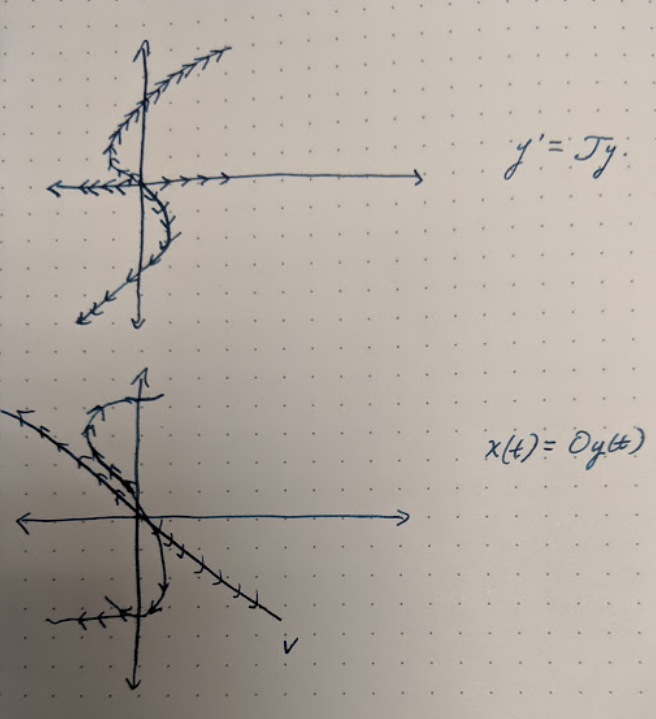
\includegraphics{7-9-1.png}

{\bf Example.} Let $A = \mat{3 & 5 & 2 \\ -7 & 9 & 3 \\ 4 & -4 & 0}$.  Find the independent solutions to $\mbf{x}' = A \mbf{x}$.

Recall that
\begin{align*}
  \det(A - \lambda I) &= \det \mat{-3 - \lambda & 5 & 2 \\ -7 & 9-\lambda & 3 \\ 4 & -4 & 0}  \\
  &= (-3 - \lambda) \det \mat{3 - \lambda & 3 \\ -4 & - \lambda} - 5 \det \mat{-4 & 3 \\ 4 & - \lambda} + 2 \det \mat{-4 & 9 - \lambda \\ 4 & -4} \\
  &= (- 3 - \lambda) \left[ (3- \lambda)(- \lambda) + 12 \right] - 5 \left[ 4 \lambda - 12 \right] + 2 \left[ 16 - 4 (9 - \lambda) \right] \\
  &= - \lambda^3 + 6 \lambda^2 - 12 \lambda + 8 \\
  &= (2 - \lambda)^3.
\end{align*}

Recall that we proved that either $A$ is diagonalizable, or that it is similar to a matrix $\mat{2 & 1 & 0 \\ 0 & 2 & 1 \\ 0 & 0 & 2}$ or $\mat{2 & 1 & 0 \\ 0 & 2 & 0 \\ 0 & 0 & 2}$.

Notice that the number of independent eigenvectors is equal to $n = \dim \Ker \left( A - 2 I \right)$.

\begin{itemize}
  \item If $n = 1$, $J = \mat{2 & 1 & 0 \\ 0 & 2 & 1 \\ 0 & 0 & 2}$.
  \item If $n = 2$, $J = \mat{2 & 1 & 0 \\ 0 & 2 & 0 \\ 0 & 0 & 2}$.
\end{itemize}

Note that
\begin{align*}
  A - 2I = \mat{-5 & 5 & 2 \\ -7 & 7 & 3 \\ 4 & -4 & -2}.
\end{align*}

Further, by the rank-nullity theorem
\begin{align*}
  3 = \dim(\ker(A - 2I)) + \dim(\ImT (A - 2I))
\end{align*}

Here, the form of $J$ is known as the Jordan canonical form.

So far, we have concluded that
\begin{align*}
  A = O \mat{2 & 1 & 0 \\ 0 & 2 & 1 \\ 0 & 0 & 2} O^{-1},
\end{align*}
where $O = \mat{\mbf{v}, \mbf{w}_1, \mbf{w}_2}$.  

\begin{itemize}
  \item To find $\mbf{v}$, just look at $(A - 2I) \mbf{v} = 0$.
  \item Once $\mbf{v}$ is found, $\mbf{w}_1$ satisfies $(A - 2I) \mbf{w}_1 = \mbf{v}$.
  \item Once $\mbf{w}_1$ is known, $\mbf{w}_2$ satisfies $(A - 2I) \mbf{w}_2 = \mbf{w}_1$.
\end{itemize}

We will skip the computation in lecture, but we obtain the following:
\begin{align*}
  \mbf{v} = \mat{1 \\ 1 \\ 0}; \qquad \mbf{w}_1 = \mat{-1 \\ 0 \\ -2}; \qquad \mbf{w}_2 = \mat{3 \\ 0 \\ 7}.
\end{align*}

Recall from yesterday, we had seen that if $\mbf{y}' = J \mbf{y}$ and $J = \mat{\lambda & 1 & 0 \\ 0 & \lambda & 1 \\ 0 & 0 & \lambda}$, it follows that
\begin{align*}
  y_1' &= \lambda y_1 + y_2 \\ 
  y_2' &= \lambda y_2 + y_3 \\
  y_3' &= \lambda y_3.
\end{align*}

Then the general solution is given by
\begin{align*}
  \mbf{y}(t) = \mat{c_3 \frac{t^2}{2} e^{2t} + c_2 t e^{2t} + c_1 e^{2t} \\ c_3 t e^{2t} + c_2 e^{2t} \\ c_3 e^{2t}}.
\end{align*}

Some example solutions include the following:
\begin{itemize}
  \item $\mbf{v}_1(t) = \mat{e^{2t} \\ 0 \\ 0}$.
  \item $\mbf{v}_2(t) = t e^{2t} \mat{ 1 \\ 0 \\ 0} + e^{2t} \mat{0 \\ 1 \\ 0}$.
  \item $\mbf{v}_3(t) = \frac{t^2}{2} e^{2t} \mat{1 \\ 0 \\ 0} + t e^{2t} \mat{0 \\ 1 \\ 0} + e^{2t} \mat{0 \\ 0 \\ 1}$.
\end{itemize}

Note that $\mbf{v}_1, \mbf{v}_2, \mbf{v}_3$ are independent solutions (check the Wronskian).  Since 

\begin{itemize}
  \item $\mbf{x} = O \mbf{y}$ satisfies $\mbf{x}' = A \mbf{x}$, 
  \item $O$ maps $\mat{1 \\ 0 \\ 0} \to \mbf{v}$, $\mat{0 \\ 1 \\ 0} \to \mbf{w}_1$, $\mat{0 \\ 0 \\ 1} \to \mbf{w}_2$. 
\end{itemize}

Three independent solutions for $\mbf{x}' = A \mbf{x}$ are given by
\begin{align*}
  \tilde{\mbf{v}}_1 &= e^{2t} \mbf{v} \\
  \tilde{\mbf{v}}_2 &= te^{2t} \mbf{v} + e^{2t} \mbf{w}_1 \\
  \tilde{\mbf{v}}_3 &= \frac{t^2}{2} e^{2t} \mbf{v} + t e^{2t} + \mbf{w}_1 + e^{2t} \mbf{w}_2.
\end{align*}

One comment about the phase portrait: recall that we saw from before if $A = \mat{2 & 1 \\ 0 & 2}$, we get a phase portrait of the following form:

Instead, consider $A = \mat{0 & 1 \\ -1 & 1 - \varepsilon}$.  Computing the eigenvalues, we obtain
\begin{align*}
  \det (A - \lambda I) &= \det \mat{- \lambda & 1 \\ - 1 & 2 - \lambda - \varepsilon} \\
  &= \lambda^2 + (-2 + \varepsilon) \lambda + 1.
\end{align*}

Computing the eigenvalues, we obtain
\begin{align*}
  \lambda = \frac{2 - \varepsilon \pm \sqrt{- 4 \varepsilon + \varepsilon^2}}{2}.
\end{align*}

We can obtain the following phase portraits; the first phase portrait is a limiting case of the second.



\section{Lecture 12: 7-10-19}

{\bf Fundamental solution and exponential of a matrix.}

Recall the problem $\mbf{x}' = A \mbf{x}$.  We know how to solve this using $A = O \Lambda O^{-1}; A = O JO^{-1}$ (using the diagonal matrix and the Jordan canonical matrix).

The solutions are given by
\begin{align*}
  \mbf{x}(t) = c_1 e^{\lambda_1 t} \mbf{v}_1 + c_2 e^{\lambda_2 t} \mbf{v}_2 + \cdots + c_n e^{\lambda_n t } \mbf{v}_n.
\end{align*}

\begin{definition}
  A fundamental matrix for a system of ODE $\mbf{x}' = A \mbf{x}$ is a matrix $X(t)$ such that for any constant vector $\mbf{c}$, we have $X(t) \mbf{c}$ is a solution of the system of ODE.  This is the same as the columns of $X(t)$ are independent solutions. 
\end{definition}

Since for all $\mbf{c}$, $X(t) \mbf{c}$ is a solution, if we want $x_0 = \mbf{x}(t_0) = X(t_0) \mbf{c}$, invert $X (t_0)$ so that $\mbf{c} = (X(t_0))^{-1} \mbf{x}_0$.  Then $X(t) X^{-1} (t_0) \mbf{x}_0$ is a solution and it satisfies the initial condition.

{\bf Example.} If $A = \mat{0 & 1 \\ 1 & 0}, \lambda = \pm 1, \mbf{v} = \mat{1 \\ 1}, \mbf{w} = \mat{-1 \\ 1}$, then $X(t) = \mat{e^{t} & -e^{-t} \\ e^{t} & e^{-t}}$ is a fundamental matrix.

If $\mbf{x}' = A \mbf{x}$ is paired with $\mbf{x}(0) = x_0$ and a fundamental matrix $X(t)$ is given, then
\begin{align*}
  \tilde{X}(t) = X(t) X^{-1}(0)
\end{align*}
is also a fundamental solution.  Therefore, if $\mbf{c} = \mbf{x}_0$, then $\tilde{X}(t) \mbf{c}$ is a solution ot the ODE, and it matches the initial condition since $\tilde{X}(0) \mbf{c} = I \mbf{x}_0 = \mbf{x}_0$.

{\bf Definition.} Given an $n \times n$ matrix $A$, its exponential $e^{tA} = \sum_{n=0}^{\infty} \frac{t^n A^n}{n!}$.

Notice that $\tilde{X}(0) = I$, since $e^{0A} = I$.  If we also check that the columns of $e^{tA}$ are solutions ot the ODE $\mbf{x}' = A \mbf{x}$, we are good.

Equivalently, $e^{tA} \mbf{c} = \mbf{y}(t)$ satisfies $\mbf{y}'(t) = A \mbf{y}(t)$.  Thus,
\begin{align*}
  (e^{tA} \mbf{c})' &= \left( \sum_{n=0}^{\infty} \frac{t^n A^n \mbf{c}}{n!} \right) \\
  &= \sum_{n=1}^{\infty} \frac{t^{n-1j A^n \mbf{c}}}{(n-1)!} \\
  &= A \sum_{n=1}^{\infty} \frac{t^{n-1}}{(n-1)!} A^{n-1} \mbf{c} \\
  &= A \sum_{m=0}^{\infty} \frac{t^m}{m!} A^m \mbf{c} = A e^{tA} \mbf{c} \\
  &= A y(t).
\end{align*}

In summary, the $\tilde{X}$ from above is exactly the same as the matrix exponential.  We now will look at some examples.

{\bf Case 1.} If $\Lambda = \text{diag}(\lambda_1, \dots, \lambda_n)$, what is $e^{tA}$?  Then
\begin{align*}
  e^{tA} = \sum_{n=0}^{\infty} \frac{t^n \Lambda^n}{n!} = \text{diag}(e^{t \lambda_1}, \dots, e^{t \lambda_n}).
\end{align*}

{\bf Case 2.} Suppose $A$ is diagonalizable, i.e. $A  O \Lambda O^{-1}$, where $\Lambda$ is diagonal.  To do this, we can write
\begin{align*}
  e^{tA} &= \sum_{n=0}^{\infty} \frac{t^n A^n}{n!} =  \sum_{n=0}^{\infty} \frac{t^n (O \Lambda O^{-1})^{n}}{n!} \\
  &= \sum_{n=0}^{\infty} \frac{t^n O \Lambda^n O^{-1}}{n!} \\
  &= O \left( \sum_{n=1}^{\infty} \frac{t^n \Lambda^n}{n!} \right) O^{-1} \\
  &= O e^{tA} O^{-1} \\
  &= O \text{diag}(e^{t \lambda_1}, \dots, e^{t \lambda_n}) O^{-1}.
\end{align*}

{\bf Case 3.} How do we compute $e^{tJ}$, where $J$ is an arbitrary Jordan canonical form?  We will start by doing the $2 \times 2$ case.

Suppose $J = \mat{\lambda & 1 \\ 0 & \lambda} = \underbrace{\mat{\lambda & 0 \\ 0 & \lambda}}_{\text{call this $\Lambda$}} + \underbrace{\mat{0 & 1 \\ 0 & 0}}_{\text{call this $N$}}$.

{\bf Key point.} If $\Lambda$ is diagonal, $N^2 = \mat{0 & 0 \\ 0 & 0}$, where $\Lambda$ and $N$ commute.  Here $N$ is nilpotent.

And using this, we can apply a sort of binomial theorem for matrices.  If $A$ and $B$ commute, then
\begin{align*}
  (A+B)^n = \sum_{k=0}^{n} \binom{n}{k} A^k B^{n-k}.
\end{align*}

(Note that this result is not true if $A$ and $B$ don't commute; things are much more complicated in that setting).

Thus,
\begin{align*}
  e^{tJ} &= \sum_{n=0}^{\infty} \frac{t^n J^n}{n!} \\
  &= \sum_{n=0}^{\infty} \frac{t^n (\Lambda + N)^n}{n!} \\
  &= \sum_{n=0}^{\infty} \frac{t^n}{n!} (A^n + n \Lambda^{n-1} N) \\
  &= \sum_{n=0}^{\infty} \frac{t^n}{n!} \Lambda^n + \sum_{n=0}^{\infty} \frac{t^n}{n!} n \Lambda^{n-1} N \\
  &= e^{t \Lambda} + t N \sum_{n=1}^{\infty} \frac{t^{n-1}}{(n-1)!} \Lambda^{n-1} \\
  &= e^{t \Lambda} (1 + tN) \\
  &= \mat{e^{\lambda t} & 0 \\ 0 & e^{\lambda t}} + t \mat{0 & t \\ 0 & 0 }\mat{e^{\lambda t} & 0 \\ 0 & e^{\lambda t}} \\
  &= \mat{e^{\lambda t} & t e^{\lambda t} \\ 0 & e^{\lambda t}}.
\end{align*}

{\bf Case 4.} If $A = O J O^{-1}$, then $e^{tA} = O e^{tJ} O^{-1}$ (same proof as case 2).

{\bf Example (complex eigenvalue case).} Suppose $A = \mat{0 & 1 \\ -1 & 0}$.  What is $e^{tA}$?

One way is to compute $\lambda_1 = i, \lambda_2 = -i$, $\mbf{v}, \mbf{w}$, and note that
\begin{align*}
  e^{tA} &= \mat{1 & 1 \\ -i & i} \mat{e^{it} & 0 \\ 0 & e^{-it}} \mat{1 & 1 \\ -i & i}^{-1} \\
\end{align*}

Also, notice that
\begin{align*}
  A^2 = \mat{0 & 1 \\ -1 & 0} \mat{0 & 1 \\ -1 & 0} = -I.
\end{align*}

Thus, if we compute the matrix exponential, we can obtain
\begin{align*}
  e^{tA} &= \sum_{n=0}^{\infty} \frac{t^n A^n}{n!} \\
  &= I + tA + \frac{t^2}{2} A^2 + \frac{t^3}{3!} A^3 + \dots \\
  &= I - \frac{I t^2}{2} + I \frac{t^4}{4!} + \dots + A\left(  t I - I \frac{t^3}{3!} + I \frac{t^5}{5!} - \dots \right) \\
  &= \cos t \mat{1 & 0 \\ 0 & 1} + \sin t \mat{0 & 1 \\ -1 & 0} \\
  &= \mat{\cos t & \sin t \\ -\sin t & \cos t}.
\end{align*}

In this way, we get two fundamental solutions which are real.

In summary, if $\mbf{x}' = A \mbf{x}$, the solution should be $e^{tA} \mbf{x}_0$.

But there are complications.  We need to check which properties are true for a mmatrix.

For example, is it true that $e^{(t+s)A} = e^{tA} e^{sA}$?  Answer is yes.  Easy way to prove this is to use the existence and uniqueness theorem for ODEs.

What about $e^{t(A+B)} = e^{tA} e^{tB}$?  Answer is no, unless $A$ and $B$ commute.  In fact, we do have equality here if and only if $A$ and $B$ commute. 

It is enough to prove that $\mbf{x} = e^{tA} e^{tB}$ satisfies $\mbf{x}' = (A+B) \mbf{x}$ and $\mbf{x}(0) = \mbf{c}$.

\section{Review: Phase Portraits of Linear Systems}

Using reference: http://www.math.psu.edu/tseng/class/Math251/Notes-PhasePlane.pdf.

While labor intensive, it is possible to sketch the phase portrait by hand without having to solve the system (do something similar to the direction field case).

Recall that an equilibrium solution is a constant solution of the system, a point $(x_1, x_2)$ where $\mbf{x}' = 0$.  In general, we will consider systems whose coefficient matrix has nonzero determinant; that is, systems whose origin is the only critical point.


(Asked Andrea); Recall we have the following cases:

\begin{itemize}
  \item $\lambda_1 < 0 \lambda_2$
  \item $\lambda, \lambda > 0$
  \item $\lambda_1, \lambda_2 < 0$
  \item $\lambda_1 =  a + ib, \lambda_2 = a - ib$.
\end{itemize}

\todo{Add images}

\section{Lecture 13: 7-11-19}

Now, we'll discuss inhomogeneous system of ODE.  That is, problems of the form
\begin{align*}
  \mbf{x}' = A \mbf{x} + \mbf{b}.
\end{align*}

Recall that the solution to this is equal to the solution of the homogeneous problem plus a particular solution.

{\bf Lemma.} If $x_1, x_2$ are two solutions of $\mbf{x}' = A \mbF{x} + b$, then $y = \mbf{x}_1 - \mbf{x}_2$ solves $\mbf{y}' = A \mbf{y}$.

\begin{proof}
  Just apply the linearity of the derivative.
\end{proof}

{\it Remark.} This idea applies to the case where $\mbf{A}, \mbf{b}$ is nonconstant as well (but of course, we don't know how to solve the problem when $A$ is nonconstant).

To find a particular solution, just note that we can find the equilibrium solution pretty easily.  If $\mbf{x}' = A \mbf{x}$, then $\mbf{x} =  0$ is a solution.

Simliarly, if $\mbf{x}' = A \mbf{x} + \mbf{b}$, with the condition $A$ is invertible, we can look for the solution $\mbf{x}_0 =- A^{-1} \mbf{b}$.

Therefore, using the lemma, the general solution of $\mbf{x}' = A \mbf{x} + \mbf{b}$ is  $\mbf{x} = - A^{-1} \mbf{b} + \mbf{X}(t) \mbf{c}$, where $X(t)$ is a fundamental matrix and $\mbf{c}$ is an arbitrary vector.

{\bf Example.} Take $A = \mat{0 & 1 \\ 1 & 0}$, and $\mbf{b} = \mat{1 \\ 2}$, $\mbf{x}_0 = \mat{0 \\ 0}$.

Then from before, we have $\lambda = \pm 1$, with $\mbf{v} = \mat{1 \\ 1}$, $\mbf{w} = \mat{1 \\ -1}$; we obtain the fundamental matrix $X(t) = \mat{e^t & e^{-t} \\ e^t & - e^{-t}}$.

Therefore, the final solution to the problem is
\begin{align*}
  \mbf{x}(t) &= X(t) \mbf{c} - A^{-1} \mbf{b} \\
  &= c_1 \mat{e^t \\ e^t} + c_2 \mat{e^{t} \\ - e^{-t}} + \mat{-2 \\ -1}.
\end{align*}

At $t = 0$, we get
\begin{align*}
  \mbf{x}(0) = c_1 \mat{1 \\ 1} + c_2 \mat{1 \\ - 1} + \mat{-2 \\ -1} = \mat{0 \\ 0}
\end{align*}
which  gives us $c_1 = \frac{3}{2}, c_2 = \frac{1}{2}$.

This gives us the final solution of
\begin{align*}
  \mbf{x}(t) = \mat{\frac{3}{2} e^ t+ \frac{1}{2}e^{-t} -2 \\ \frac{3}{2} e^t - \frac{1}{2} e^{-t} - 1 }.
\end{align*}

For the phase portrait, just shift the phase portrait of $\mbf{x}' = A \mbf{x}$ by the vector $- A^{-1} \mbf{b}$.

What about the general solution for $\mbf{x}' = A \mbf{x} + \mbf{g}$, where $\mbf{g}$ is a function of $t$? Intuitively, you have a system and there's a force that acts in a nonconstant way on the system (e.g. temperature in some room).

{\bf Idea.} We just need a particular solution; then just add the solution to the homogeneous problem.

Let's try applying the integrating factor idea from before; this is one reason we introduced the exponential of a matrix.  We rewrite the ODE in the form
\begin{align*}
  \mbf{x}' - A \mbf{x} = g,
\end{align*}
and multiply by $e^{-tA}$.  We note that $e^{-tA}$ is always invertible because the columns are a solution of the ODE and at time $t = 0$, $e^{-0A} = I$.  Alteernatively, we can realize that if $A = O \Lambda O^{-1}$, and that $e^{-tA} = O e^{-tA} O^{-1}$.

Multiplying on the left, we obtain
\begin{align*}
  e^{-tA} \mbf{x}' - e^{-tA} A \mbf{x} = e^{-tA} \mbf{g}.
\end{align*}
Thus,
\begin{align*}
  - e^{tA} \mbf{x} ' - e^{-tA} A \mbf{x} = e^{-tA} \mbf{g}.
\end{align*}
Importantly, $e^{-tA}$ commutes with $A$, since from the power series expansion $A$ should commute with powers of itself.

This is the same as
\begin{align*}
  (e^{-tA} \mbf{x})'  = e^{-tA} \mbf{g}.
\end{align*}

Integrating, we obtain
\begin{align*}
  e^{-tA} \mbf{x} = \mbf{c} + \int^{t} e^{-sA} \, g(s) \, ds.
\end{align*}

And in conclusion,
\begin{align*}
  \mbf{x}(t) = e^{tA} \mbf{c} + e^{tA} \int^{t} e^{-sA} g(s) \, ds.
\end{align*}

{\bf Remark 1.} The solution is $\mbf{x}(t) = e^{tA} \mbf{s} + e^{tA} \int^{t} e^{-sA} \, g(s) \, ds$.

{\bf Remark 2.} Recall that the integrating factor $\mu(t)$ is non-unique (since you can start the integral from where you want due to invariance under constant multiplication).

Here, instead of $e^{At}$ we use any fundamental matrix $X(t)$, then $X(t)$ is always invertible (using the Wronskian argument), and also $\frac{d}{dt} X(t) = A X(t)$. Here, the previous relation is the same as $(\mbf{v}', \mbf{w}') = (A \mbf{v}, A \mbf{w})$.

Therefore, $\mbf{x}(\mbf{c}) = X(t) \mbf{c} + X(t) \int^{t} X^{-1}(s) g(s) \, ds$.

{\bf Remark 3.} If $A$ is not-constant, but somehow we know a fundamental matrix $X(t)$, then the argument works the same.

{\bf Example.} Solve the problem $\mbf{X}' = \mbf{A} \mbf{x} + \mbf{g}$, where $A = \mat{1 & -4 \\ 2 & -5}$, $\mbf{x}(0) = \mat{3 \\ 5}$, $\mbf{g}(t) = \mat{e^t \\ e^{-t}}$.  Find $\mbf{x}(t)$.

First, we find the fundamental matrix, and use the formula from above.  To find $X(t)$, we compute the eigenvalues of $A$.  Computing, we obtain
\begin{align*}
  \det (A - \lambda I) &= (1 - \lambda)(-5 - \lambda) + 8 = 0 \\
  &= (\lambda^2 + 4\lambda + 3) = (\lambda + 3)(\lambda + 1) = 0.
\end{align*}

Thus $\lambda = -1, -3$.  Now, if $\mbf{v}$ is relative to $\lambda_1 = -3$, we obtain $\mbf{v} = \mat{1 \\ 1}$.  Similarly, if $\mbf{w}$ is relative to $\lambda_2 = -1$, we obtain $\mat{1 & -4 \\ 2 & -5} \mat{v_1 \\ v_2} = \mat{- v_1 \\ - v_2}$, so that $2 v_2 - 4v_2 = 0$, and $\mbf{w} = \mat{2 \\ 1}$.

Thus, the fundamental matrix is
\begin{align*}
  X(t) = \mat{e^{-3t} & 2 e^{-t} \\ e^{-3t} & e^{-t}}.
\end{align*}

Computing the inverse, note that
\begin{align*}
  X^{-1}(t) = \frac{1}{e^{-2t} - 2 e^{-4t}} \mat{e^{-t} & e^{-3t} \\ -2 e^{-t} & e^{-3t}} = \mat{- e^{3t} & e^{3t} \\ e^t & - e^t}.
\end{align*}

Thus, the final solution is
\begin{align*}
  \mbf{x}(t) &= c_1 \mat{e^{-4t} \\ e^{-3t}} + c_2 \mat{2 e^{-t} \\ e^{-t}} + \mat{e^{-3t} & 2e^{-t} \\ e^{-3t} & e^{-t}} \int^{t} \mat{- e^{3s} & e^{3s} \\ e^{s} & - e^{s}} \mat{e^s \\ e^{-s}} \, ds.
\end{align*}

The final result is
\begin{align*}
  \mbf{x}(t) &= c_1 \mat{e^{-3t} \\ e^{-3t}} + c_2 \mat{2 e^{-t} \\ e^{-t}} + \mat{e^{-3t & 2 e^{-t} \\ e^{-3t} & e^{-t}}} \mat{- \frac{1}{4} e^{4t} + \frac{1}{2} e^{2t} \\ \frac{1}{2} e^{2t} - t} \\
  &= c_1 \mat{e^{-3t} \\ e^{-3t}} + c_2 \mat{2 e^{-t} \\ e^{-t}} + \mat{- \frac{1}{4} e^t + \frac{1}{2} e^{-t} + e^t - 2e^{-2t} \\ - \frac{1}{4} e^{t} + \frac{1}{2} e^{-t} + \frac{1}{2} e^t + t e^{-t}}.
\end{align*}

To solve the initial value problem, just plug in $t = 0$.

In the last part of class, we'll discuss the setting in which $A$ is non-constant.  That is, can we solve $\mbf{x}'(t) = A(t) \mbf{x}(t)$?  

In the scalar case, if $y' = p(t) y$, then $y(t) = c e^{\int^t p(s) \, ds}$.

{\bf Guess.} For the matrix case, let's try to do the same thing.  If $B(t) = \int^{t} A(s) \, ds$, then is $e^{B(t)}$ is a solution?

The problem is that it does not, which probably indicates a commutativity issue.  To see why, notice that we require the following equality, which turns out to be false.
\begin{align*}
  \frac{d}{dt} \left( e^{B(t)} \right) = B'(t) e^{B(t)} = A(t) e^{B(t)}.
\end{align*}

We start by taking the derivative, that is
\begin{align*}
  \frac{d}{dt} \left( e^{B(t)} \right) = \sum_{n=0}^{\infty} \frac{d/dt (B(t))^n}{n!}.
\end{align*}

But, even for $n = 2$, note that $\frac{d}{dt} (B^2(t)) \neq 2 B'(t) B(t)$.  We actually get
\begin{align*}
  \frac{d}{dt} B^2(t) = B'(t) B(t) + B(t) B'(t).
\end{align*}

(Note, this stuff won't be on exam / homework.)

{\bf Remark.} Note that this problem is solvable if we have the condition $A(t) A(s) = A(s) A(t)$.

\section{Lecture 14: 7-12-19}

Today, we'll consider non-linear systems of ODEs.  Previously, we solved the problem
\begin{align*}
  \mbf{x}' = A \mbf{x}; \qquad \mbf{x}' = A \mbf{x} + b.
\end{align*}
Now, we want to understand $\mbf{x}' = f (\mbf{x})$.  Note that if
\begin{align*}
  f(x, y) = \mat{f_1(x, y) \\ f_2(x, y)} = \mat{x(1 - x - y) \\ y(\frac{3}{4} - y - \frac{1}{2}x)}.
\end{align*}
Then
\begin{align*}
  \mat{\frac{dx}{dt} \\ \frac{dy}{dt}} = \mat{x(1 - x - y) \\ y(\frac{3}{4} - y - \frac{1}{2}x)}.
\end{align*}

Intuitively, we can understand this setting as the dynamics between two competing species, where
\begin{itemize}
  \item $x(t)$ is the # of wolves
  \item $y(t)$ is the number of foxes
\end{itemize}

{\bf Ideas.}

\begin{itemize}
  \item Understand equilibria of the system; that is find $\mat{x \\ y}$ constant vector or $f(x, y) = 0$.
  \item Understand the nature of the equilibria $\to$ understand $\mbf{x}(t)$ where $\mbf{x}(0)$ is close to an equilibrium.  This tool is called linearization.
\end{itemize}

More ambitiously, we can understand the global behavior of the system.

What are the equilibria for $\mbf{x} ' = f(x)$.  Note that $\mat{x \\ y}$ is an equilibrium if
\begin{align*}
  \mat{x(1 - x - y) \\ y (\frac{3}{4} - y - \frac{1}{2}x)} = \mat{0 \\ 0}.
\end{align*}

If $x = 0$, we get the equilibria of either $(0, 0); (0, \frac{3}{4})$.

Otherwise, $1 - x - y = 0$, which implies $x = 1-y$, that is
\begin{align*}
  y (\frac{3}{4} - y - \frac{1}{2} ( 1 - y)) = 0,
\end{align*}

giving us the equilibria of either $(1, 0), (\frac{1}{2}, \frac{1}{2})$.

Now, we need to understand the phase portrait around the equilibria.

If $\mbf{x}_0$ is an equilibrium, then $f(\mbf{x}_0) = \mbf{0}$.  If $\mbf{x}$ is close to $\mbf{x}_0$, then $f(\mbf{x}) \approx f(\mbf{x}_0) + J( \mbf{x} - \mbf{x}_0 )$, where $J$ is the Jacobian matrix of the function.

Recall that the Jacobian is the matrix where
\begin{align*}
  J_{ij} = \frac{\partial f_i}{\partial x_j}.
\end{align*}

So in this case,
\begin{align*}
  J_f(\mbf{x}_0) = \mat{\frac{\partial f_1}{\partial x} & \frac{\partial f_1}{\partial y} \\ \frac{\partial f_2}{\partial x} & \frac{\partial f_2}{\partial y}}(\mbf{x}_0).
\end{align*}

So, around $\mbf{x}_0$, we have
\begin{align*}
  \mbf{x}' \approx f(\mbf{x}_0) + J_f(\mbf{x}_0) (\mbf{x} - \mbf{x}_0).
\end{align*}

In other words, this is using the tangent plane to approximate the multivariate function.

Now, we found four equilibria; and we have to linearize around them to obtain a phase portrait.

First, compute the Jacobian.  We have that

\begin{align*}
  J_f( (x, y) ) = \mat{1 - 2x -y & -x \\ -\frac{y}{2} & \frac{3}{4} - 2y - \frac{x}{2}}
\end{align*}

How does the phase potrait look around $(0, 0)$?  Should be the same as $\mbf{x}' = \mat{1 & 0 \\ 0 & \frac{3}{4}} \mbf{x}$.  And we know how to plot the phase portrait for this system.  We note that

\begin{align*}
  \lambda_1 = 1, \lambda_2 = \frac{3}{4};
\end{align*}
\begin{align*}
  \mbf{v}_1 = \mat{1 \\ 0}; \qquad \mbf{v}_2 = \mat{0 \\ 1}.
\end{align*}

And we recall that the phase portrait looks like a parabola.

What about (1, 0)?  Substituting, we obtain
\begin{align*}
  J_f(1, 0) = \mat{-2 & -1 \\ 0 & \frac{1}{4}}.
\end{align*}

Thus
\begin{align*}
  \mbf{x}' = \mat{-1 & -1 \\ 0 & \frac{1}{4}} \mat{ \mbf{x} - \mat{1 \\ 0}}.
\end{align*}

Solving for the eigenvectors, we have $\lambda_1 = -1, \lambda_2 = \frac{1}{4}$.  And for the eigenvectors, we obtain $\mbf{v} = \mat{1 \\ 0}, \mbf{w} = \mat{4 \\ -5}$.

We can plot this as the hyperbolic case (saddle).

The equilibrium $(0, \frac{3}{4})$ is pretty simple.  The interesting stuff is what happens at the equilibrium $(\frac{1}{2}, \frac{1}{2})$.

In this case, we have
\begin{align*}
  \mbf{x}' \approx \mat{- \frac{1}{2} & - \frac{1}{2} \\ - \frac{1}{4} & - \frac{1}{2}} \mat{\mbf{x} - \mat{1 \\ 2}}
\end{align*}

Computing the eigenvalues, we obtain
\begin{align*}
  \det (A - \lambda I) = \det \mat{- \frac{1}{2} - \lambda & - \frac{1}{2} \\ - \frac{1}{4} & - \frac{1}{2} - \lambda} = \lambda^2 + \lambda + \frac{1}{4} - \frac{1}{8} = \lambda^2 + \lambda + \frac{1}{8}.
\end{align*}

So the roots are
\begin{align*}
  \lambda &= \frac{- 1 \pm \sqrt{1 - \frac{1}{2}}}{2} = \frac{-1 \pm \frac{\sqrt{2}}{2}}{2} \\
  &= \frac{-2 \pm \sqrt{2}}{4}.
\end{align*}

Since both eigenvalues are negative, the picture is qualitatively stable.  And then, assuming continuity and uniqueness, we should guess that we can ``interpolate'' between the phase portraits we know how to solve to plot the full phase portrait.

Globally, it turns out that the phase portrait will converge to $ (\frac{1}{2}, \frac{1}{2})$, unless you have $0$ wolves or $0$ foxes.

To show this, we can study the direction field.  If we have the problem $\mat{x' \\ y'} = \mat{x(1-x-y) \\ y(\frac{3}{4} - y - \frac{x}{2})}$.

If the components are positive, we know that the direction field is increasing.  We can draw all the 4 cases based on the signs of the components.

If $x(1 - x - y) > 0, y(\frac{3}{4} - y- \frac{x}{2} ) > 0$, direction field goes northeast.

If $x' < 0, y' > 0$, direction goes northwest.

If $x' > 0, y' < 0$, direction goes southeast.

If $x' < 0, y' < 0$, direction goes southwest.

Sometimes, it is possible to get complicated oscillations and cycles.  But in this case, we happen to know that we won't get these.

In this example, we did two competing species (both predator).

We can consider a more complicated setting where we have prey and predator.  That is,
\begin{align*}
  \mat{x' \\ y'} = \mat{x (1 - 2y) \\ y(- \frac{3}{4} + \frac{1}{x})}.
\end{align*}

In this case, $y$ represent the predator (naturally tends to die), and $x$ represents the prey (naturally tends to grow).

To solve for the equilibria, we consider the cases:

\begin{itemize}
  \item $x = 0$, $y= 0$.
  \item $x = 3, y = \frac{1}{2}$ (will be a center).
\end{itemize}

Computing, we obtain
\begin{align*}
  J_f(x, y) = \mat{1 - 2y & -2x \\ \frac{y}{4} & \frac{x}{4} - \frac{3}{4}}
\end{align*}

So, at $(0, 0)$, $J_f(0, 0) = \mat{1 & 0 \\ 0 & - \frac{3}{4}}$.  Here, the eigenvalues are $1, -\frac{3}{4}$, with eigenvectors $\mat{1 \\ 0}, \mat{0 \\ 1}$.

At $(3, \frac{1}{2})$, $J = \mat{0 & -6 \\ \frac{1}{8} & 0}$.  Computing the eigenvalues, $\lambda^2 = - \frac{3}{4}$, thus $\lambda = \pm \frac{\sqrt{3}}{2} i$.  This is the case where $\alpha = 0$, so this will trace out an ellipse.

But note that it could be the case where a small perturbation results in a nonlinearity.  In this case, we can actually show that this isn't true, but it is a concern.

Next week, when we discuss separable equations, we will discuss how to obtain the exact shape of these curves.

Let's try to convince ourselves that going circularly around the equilibrium $(3, \frac{1}{2})$ works in terms of the direction field.

The error of the linear approximation is related to the second derivative.  So if $f$ is a crazy function, this might have significant errors.

\section{Lecture 15: 7-15-19}

Came in late, summarizing key parts of lecture.

{\bf Example.} Suppose $\frac{dy}{dt} = \frac{t^2}{1 - y^2}$, $y(0) = 0$.  Then

\begin{align*}
  dy(1-y^2) = dt t^2,
\end{align*}
so
\begin{align*}
  y - \frac{y^3}{3} = \frac{t^3}{3} + C,
\end{align*}
and plugging in the initial condition, we obtain $C = 0$.

{\bf Example.} Suppose
\begin{align*}
  \frac{dy}{dt} = \frac{3t^2 + 4t + 2}{2(y-1)},
\end{align*}
with $y(0) = y_0$.

Then
\begin{align*}
  2(y-1) dy = (3t^2 + 4t + 2) \, dt,
\end{align*}
that is
\begin{align*}
  y^2 - 2y = t^3 + 2t^2 + 2t + C.
\end{align*}

Plugging in initial condition, we get
\begin{align*}
  y_0^2 - 2y_0 = C,
\end{align*}
so
\begin{align*}
  y^2 - 2y = t^3 + 2t^2 + 2t + y_0^2 - 2y_0.
\end{align*}

We can solve for $y$ using quadratic formula, that is
\begin{align*}
  y^2 - 2y + 1 = t^3 + 2t^2 + 2t + y_0^2 - 2y_0 + 1.
\end{align*}

Then
\begin{align*}
  y(t) = \pm \sqrt{t^3 + 2t^2 + 2t + y_0^2 - 2y_0 + 1} + 1.
\end{align*}


At least for $t$ small (so that $\sqrt{}$ is defined), we get two solutions to the ODE.  Only one matches the initial condition.

{\bf Part a).} And given $y_0= 2$, we get  $y(t) = 1 \pm \sqrt{t^3 + 2t^2 + 2t + 1}$.

\begin{align*}
  y(t) = 1 + \sqrt{1 + t^2 + 2t^2 + 2t},.
\end{align*}

{\bf Part b).} And given $y_0 = 0$, we get $y(t) = 1 \pm \sqrt{t^3 + t^2 + 2t + 1}$.  In that case $y(t) = 1 - \sqrt{t^3 + 2t^2 + 2t + 1}$.

{\bf Part c).} And given $y_0 = 1$, we get  $y(t) = 1 \pm \sqrt{t^3 + 2t^2 + 2t}$.  We have two distinct solutions to the ODE.

\section{Lecture 16: 7-16-19}

This lecture focuses on midterm review.

Let $A = \mat{0 & 2 \\ 2 & 0}$.  Calculate the eigenvectors and eigenvalues, and $e^{tA}$.

We obtain $\lambda = \pm 2$, and $\mbf{v}_1 = \mat{1 \\ 1}, \mbf{v}_2 = \mat{1 \\ -1}$.

Now,
\begin{align*}
  e^{tA} = \mat{e^{2t} & e^{-2t} \\ e^{2t} & - e^{-2t}} \mat{1 & 1 \\ 1 & -1}^{-1},
\end{align*}
we obtain
\begin{align*}
  \mat{\frac{1}{2} \left( e^{2t} + e^{-2t} \right) & \frac{1}{2} (e^{2t} - e^{-2t}) \\ \frac{1}{2} ( e^{2t} - e^{-2t}) & \frac{1}{2} ( e^{2t} + e^{-2t})}.
\end{align*}

Recall that if we ask for the general solution of $\mbf{x}' = A \mbf{x}$, we write down
\begin{align*}
  \mf{x}(t) = c_1 \mat{e^{2t} \\ e^{2t}} + c_2 \mat{e^{-2t} \\ - e^{-2t}}.
\end{align*}

Without computing the determinant, we know that this matrix is invertible, since the eigenvalues are distinct.

There are multiple ways to see that this is invertible, since $e^{tA} = O e^{tA} O^{-1}$.

Let $\mbf{x}' = A \mbf{x} + \mat{e^t \\ e^{-t}}$, where $\mbf{x}(0) = \mat{0 \\ 0}$.  What is the solution to this IVP?

We just add $A^{-1} b$ to the solution we just got.  That is, take $\frac{1}{2} \mat{0 & 1 \\ 1 & 0} \mat{e^t \\ e^{-t}}$.

First, we can determine the general solution from before,
\begin{align*}
  \mbf{x}(t) = c_1 \mat{e^{2t} \\ e^{2t}} + c_2 \mat{e^{-2t} \\ - e^{-2t}} + X(t) \int^{t} X^{-1} (s) q(s) \, ds.
\end{align*}

So $X^{-1}(t) = \frac{1}{2} \mat{e^{-2t} & e^{-2t} \\ e^{2t} & e^{-2t}}$.  And we can compute to get the result.

{\bf Example.} Let $A = \mat{7 & -5 & -2 \\ 3 & -1 & -1 \\ 1 & -1 & 2}$, $\mbf{v} = \mat{1 \\ 1 \\ 0}$, $\mbf{w} = \mat{2 \\ 1 \\ 0}$.

Compute $A \mbf{v}$, and compute $(A - 3I)^2 \mbf{w}$.

We have that
\begin{align*}
  A \mbf{v} = \mat{2 \\ 2 \\ 0},
\end{align*}
so $\mbf{v}$ is an eigenvector with eigenvalue 2.

Also,
\begin{align*}
  (A - 3I)^2 \mbf{w} &= \mat{4 & -5 & -2 \\ 3 & -4 & -1 \\ 1 & -1 & -1}^2 \mat{2 \\ 1 \\ 0} \\
  &= 0.
\end{align*}

Find the Jordan canonical form.  To compute it, use the eigenvalues, eigenvectors, and generalized eigenvectors.

Remember when we write $A = O J O^{-1}$, we know that the columns of $O$ are eigenvectors or generalized eigenvectors.  To construct $J$, put the eigenvalues in the diagonal; and if you have a generalized eigenvector, you put a 1 above.

Since $(A - 3 I) \mbf{w} = \mat{3 \\ 2 \\ 1} \neq 0$, $\mbf{w}$ is a generalized eigenvector with eigenvalue 3.  Since $(A - 3I) \mat{3 \\ 2 \\ 1} = (A - 3I)^2 \mbf{w} = 0$, we know $\mat{3 \\ 2 \\ 1}$ is an eigenvector with eigenvalue $3$.  So if you have a generalized eigenvector of order $k$, you can get $k-1$ generalized eigenvectors (of which the last eigenvector is a a genuine eigenvector).

Now, the final decomposition is
\begin{align*}
  A = \mat{1 & 3 & 2 \\ 1 & 2 & 1 \\ 0 & 1 & 0} \mat{2 & 0 & 0 \\ 0 & 3 & 1 \\ 0 & 0 & 3} \mat{1 & 3 & 2 \\ 1 & 2 & 1 \\ 0 & 1 & 0}^{-1}.
\end{align*}

You should put the generalized eigenvector last in the columns of $O$, and in increasing order.  The matrix $O$ is invertible, because distinct eigenvalues implies eigenvectors (including generalized ones) are independent.

\begin{proof}
  Let's say $\mbf{v}$ satisfies $(A - \lambda) \mbf{v} = 0$ and $\mbf{w}$ satisfies $(A - \lambda)^2 \mbf{w} = 0$, $(A - \lambda) \mbf{w} \neq 0$.  Then, if you have the system
  \begin{align*}
    c_1 \mbf{v} + c_2 \mbf{w} = 0,
  \end{align*}
  and we apply $(A - \lambda)$, we get $c_2 (A - \lambda) \mbf{w} = 0$, so $c_2 = 0$.  Thus $\mbf{v}, \mbf{w}$ are linearly independent.

  More generally, you have to apply $(A-\lambda_1)(A - \lambda_2)$, (or the powers of products of $(A - \lambda_i)$), and you kill each vector separately.
\end{proof}

We will talk about phase portraits on Thursday.

{\bf Example.} Let's consider the problem $ty' - y = 1$, with $y(1) = 0$.  Solve the IVP.

This is just a linear ODE equivalent to $y' - \frac{y}{t} = \frac{1}{t}$, and $\mu(t) = \exp \left( \int (-\frac{1}{t}) \, dt \right)$, so $\mu(t)= \frac{1}{t}$.  Then

\begin{align*}
  \frac{y'}{t} - \frac{y}{t^2} = \frac{1}{t^2},
\end{align*}
so
\begin{align*}
  (\frac{y}{t})' = \frac{1}{t^2},
\end{align*}
and
\begin{align*}
  \frac{y}{t} = - \frac{1}{t}  +C,
\end{align*}
so that
\begin{align*}
  y = - 1 + tC.
\end{align*}
Since $y(1) = 0$, we conclude that $C = 1$ and the solution is $y = -1 + t$.  This is the unique solution in the interval $(0, \infty)$ (since there is a discontinuity at $t = 0$).

If $ty' - y = 1, y(0) = 0$, we cannot solve this, since at $t = 0$, we always get $-1$.  There is no solution.  And if we set $y(0) = -1$, we have infinitely many solutions (since we can choose any value of $C$.)

{\bf Question.} How many solutions does $y' - \frac{e^{-t^2}}{\cos t} y = e^{2t - \cos t}$, $y(37) = 54$.  We only need $p$ and $q$ continuous.  We only need to check $\cos t \neq -2$, but this never happens.  So this problem has only 1 solution on the whole line.

{\bf Definition.} Recall how to compute the matrix exponential.  If $e^{tA}$, then $e^{tA} = X(t) X^{-1}(0)$ where $X(t)$ is a fundamnetal solution for $A$.  Alternatively, we can observe that $e^{tA} = O e^{t \Lambda} O^{-1}$.  Note that $e^{tA}$ is the uniqu ematrix satisfying $\mbf{x}' = A \mbf{x}$ with $\mbf{X}(0) = Id$.

On Thursday, we'll cover phase portraits / direction fields.  Andrea will put practice exam

\section{Review for midterm}

\begin{itemize}
  \item Direction fields for scalar ODEs.

  \item Linear scalar ODEs: existence and uniqueness theory, integrating factors.

  \item Complex numbers (no branch cut).

  \item Basic notions of linear algebra: determinant, inverse matrix, eigenvalues, eigenvectors, generalized eigenvectors, diagonal/Jordan canonical form, exponential of a matrix.

    \todo{Review the JCF, and how it is used to solve an ODE / system.}


  \item  Linear system of ODEs of the form x'=Ax, x'=Ax+b, for A a constant matrix and b a constant vector. General solution and solution to the initial value problem. Associated phase portraits. Wronskian, fundamental set of solutions, fundamental matrix.

    A fundamental matrix is a matrix valued function $X(t)$ where the columns are linearly independent solutions of the system.

    \todo{Review phase portraits}

  \item  Linear inhomogeneous systems of the form x'=Ax+b(t): solution via variation of parameters (i.e., integrating factors for system of ODEs).

    Recall that the solution is
    \begin{align*}
      \mbf{x}(t) = \mbf{x}_{hom}(t) + X(t) \int^{t} X^{-1} (s) q(s) \, ds.
    \end{align*}

    Suppose we have the problem $\mbf{x}' = A \mbf{x} + \mbf{g}(t)$.  With the matrix exponential, we obtain
    \begin{align*}
      e^{-tA} \mbf{x}' - e^{-tA} A \mbf{x} = e^{-tA} \mbf{g}.
    \end{align*}
    Now, the columns of $e^{-tA}$ solve the problem $A \mbf{x} = \mbf{x}'$, so the above equation reduces to
    \begin{align*}
      (e^{-tA} \mbf{x})' = e^{-tA} \mbf{g},
    \end{align*}
    and therefore
    \begin{align*}
      e^{-tA} \mbf{x} = \int^{t} e^{-sA} g(s) ds + \mbf{c}.
    \end{align*}
    In particular,
    \begin{align*}
      \mbf{x} = e^{tA} \mbf{c} + e^{tA} \int^{t} e^{-sA} \mbf{g}.
    \end{align*}
    \todo{Derive this in the same form as linear ODE}
\end{itemize}


\section{Lecture 17: 7-17-19}

Let $y' = f(t, y)$, where $y(t_0) = y_0$.

{\bf Theorem 1.} If $f$ is continuous in a neighborhood of $(t_0, y_0)$, then $\exists $ at least one solution to the above equation for $(t-t_0)t$ small enough.

{\bf Theorem 2.} If $f, \frac{df}{dy}$ are continuous in a neighborhood of $(t_0, y_0)$, then there exists a unique solution for $(t - t_0)$ small enough.

Various examples to guarantee existence / uniqueness.

{\bf Remark 1.} For $y' + p(t) y = q(t)$, the old theorem said ``if $p, q$ are continuous at $t_0$, the exists a unique solution.

In this case, $f(t, y) = -p(t) y + q(t)$, and $\frac{\partial f}{\partial y} = - p(t)$, so the continiuity of $f$ and it's derivative is equivalent to $p, q$ continuous.

Consider $y' = y^2, y(0) = y_0 \neq 0$.  Recall that we can solve this with separation of variables.

Counterexample, consider $y'  1$ if $y \geq 0$, $y' = -1$ if $t < 0$.  There is no solution that is differentiable (absolute value doesn't work).

Stable / unstable equilibrium.  If you start from near the equilibrium, you escape (unstable), and stable means converge to an equilibrium.

\begin{itemize}
  \item If $f'(c) > 0$, then $c$ is an unstable equilibrium.
  \item If $f'(c) < 0$, then $c$ is a stable equilibrium.
  \item If $f'(c) = 0$, we cannot say anything.
\end{itemize}

Example, if $y' = y(1 - y) = f(y)$, you know that the equilibria are solutions to $y(1-y) = 0$, where $y = 0, y = 1$.

{\bf Example.} Suppose $y' = r \left( 1 - \frac{y}{K} \right) y$, where $r$ is the birthrate, where the max capacity is $K$.

Recall that to integrate do fraction decomposition: $\frac{1}{(1-y)y} = \frac{A}{y} + \frac{B}{1-y}$.

This lecture concludes first order ODEs.  Tomorrow we'll do review, Friday there's a midterm, and next week there are second order ODEs.


\section{Lecture 18: 7-18-19 (Midterm review)}

Recall that generalized eigenvectors are associated with repeated eigenvalues.

{\bf Problem 1.}

Now, to find the fundamental solution of $y' = J y$, we get the system

\begin{align*}
  a'(t) &= 2 a(t) \\
  b'(t) &= 3 b(t) + c(t) \\
  c'(t) = 3 c(t).
\end{align*}

Solving, we easily obtain $a(t) = c_1 e^{2t}$, $c(t) = c_3 e^{2t}$.  To solve for $b(t)$, we know that $b(t) = f(t) + c_2 e^{3t}$, where $c_2 e^{3t}$ is a solution to the homogeneous problem, and $f(t)$ is a particular function.

In this case, integrating factor is $e^{-3t}$, and this gives us

\begin{align*}
  (b(t) e^{-3t})' = c_3.
\end{align*}

Thus $b(t) = c_3t e^{3t} + c_2 e^{3t}$.

Idea: if $y(t)$ is a solution to $y' = J y$, then $x(t) = O y(t)$ is a solution to $x' = A x$.

Now, if $y_1, y_2, y_3$ are three independent solutions to $y' = Jy$, then $O y_1, O y_2, Oy_3$ are independent solutions to $x' = Ax$.

Obvious idea, want to check if
\begin{align*}
  \mat{e^{2t} \\ 0 \\ 0}, \mat{0 \\ e^{3t} \\ 0}, \mat{0 \\ t e^{3t} \\ e^{3t}}
\end{align*}

in independent.  At time 0, the matrix is
\begin{align*}
  \mat{1 & 0 & 0 \\ 0 & 1 & 0 \\ 0 & 0 & 1},
\end{align*}
and this is clearly invertible (since determinant is not zero; identity matrix).

There is some subtlety; got to check that $O$ is invertible (and compute the determinant).

{\bf Problem 2.}

(a) The eigenvalues are $1 \pm \sqrt{a}$.

(b) If $a = -1$, eigenvalues $1 \pm i$, so the phase portrait is an outward spiral.

If $a = 0$, then eigenvalue is $1$, you have an unstable equilibrium.

If $a = \frac{1}{4}$, then the eigenvalues are $1 \pm \frac{1}{2} = \frac{1}{2}, \frac{3}{2}$.

{\bf Problem 3.}

(a) Computation.

(b) 

{\bf Problem 4.}

(a) False.

(b) False.

(c) False. (e.g. $y' = t$).

Recall, stuff like $x' = A x + g(t)$ will be on the midterm.  Use integrating factor for matrices.

Recall that $y' + p(t) y = q(t)$, $y(t_0) = y_0$, you have existence an uniqueness  as long as $p, q$ are continuous (in an interval around $t_0$).
 
\section{Midterm practice}

\subsection{Review A}
\begin{itemize}
  \item Direction fields for scalar ODEs.

    Just plug in slopes for scalar ODEs, and draw the vectors with those slopes at each point.

  \item Linear scalar ODEs: existence and uniqueness theory, integrating factors.

    If $y' + p(t) y = q(t)$, with $y(t_0) = y_0$, we have existence and uniqueness as long as $p, q$ are continuous (in an interval around $t_0$).

  \item Complex numbers (no branch cut).

    Pretty simple.  The main thing to review is $\log z_1$ and $z_1^{z_2}$.  Remember that

    \begin{align*}
      \log z = \log r + i \theta.
    \end{align*}

    Now,
    \begin{align*}
      z_1^{z_2} &= (e^{\log z_1})^{z_2} \\
      &= e^{z_2(\log z_1)}.
    \end{align*}


  \item Basic notions of linear algebra: determinant, inverse matrix, eigenvalues, eigenvectors, generalized eigenvectors, diagonal/Jordan canonical form, exponential of a matrix.

    \begin{itemize}
      \item Eigenvalues / eigenvectors satisfy $Av = \lambda v$.
      \item Generalized eigenvectors.  A vector $v$ is a GE if $(A - \lambda I)^k v = 0$ for some integer $k$.
      \item Diagonalization.  Recall that a matrix is diagonalizable iff it has $n$ linearly independent eigenvectors.
      \item Any matrix $A$ can be put into JCF with a similarity transform.  That is, $A = O J O^{-1}$, where $O$ is invertible, and
        \begin{align*}
          J &= \diag(J_1, J_2, \dots, J_q),
        \end{align*}
        where $J_i$ is a block defined as follows:
        \begin{align*}
          J_i = \mat{\lambda_i & 1 & & & \\ & \lambda_i & \ddots & & \\ & & \ddots & 1 & \\ & & & \lambda_i}.
        \end{align*}
      \item Exponential of a matrix $e^{A} = 1 + A + \frac{A^2}{2!} + \frac{A^3}{3!} + \dots$.  The easiest way to compute this is diagonalization (when a matrix is diagonalizable).

        Other cases include the nilpotent case (which ends up being a finite sum of matrix powers).

        Alternatively, it is possible to do with JCF decomposition.

    \end{itemize}

    \todo{Review the JCF, and how it is used to solve an ODE / system.}


  \item  Linear system of ODEs of the form x'=Ax, x'=Ax+b, for A a constant matrix and b a constant vector. General solution and solution to the initial value problem. Associated phase portraits. Wronskian, fundamental set of solutions, fundamental matrix.

    \begin{itemize}
      \item $x ' = Ax$ is relatively easy to solve.

        \begin{itemize}
          \item If eigenvalues are both real, then solution is
            \begin{align*}
              c_1 e^{\lambda_1 t} \mbf{v}_1 + c_2 e^{\lambda_2 t} \mbf{v}_2.
            \end{align*}
          \item If eigenvalues are both complex, the solution is
            \begin{align*}
              c_1 e^{\lambda_1 t} \mbf{v}_1 + c_2 e^{\lambda_2 t} \mbf{v}_2,
            \end{align*}
            and then have to take real and imaginary parts of this solution to get a linearly independent combination of real solutions.
          \item If eigenvalues are repeated but there are two linearly independent vectors, then solution is just
            \begin{align*}
              c_1 e^{\lambda t} \mbf{v}_1 + c_2 e^{\lambda t} \mbf{v}_2.
            \end{align*}

          \item If eigenvalues are repeated but eigenvalues are not linearly independent, then solution is a bit different.
        \end{itemize}
      \item To solve $x' = Ax + b$, we have to find a particular solution $- A^{-1} b$, and then add this to the general solution of the homogeneous problem.

      \item Phase portraits \todo{Got to review}
      \item Fundamental set of solutions; this is a set of $n$ solutions in the $n \times n$ that are linearly independent. 
      \item Fundamental matrix, this is a matrix whose columns are linearly independent solutions of the system.
    \end{itemize}

    A fundamental matrix is a matrix valued function $X(t)$ where the columns are linearly independent solutions of the system.

    \todo{Review phase portraits}

  \item  Linear inhomogeneous systems of the form x'=Ax+b(t): solution via variation of parameters (i.e., integrating factors for system of ODEs).

    Recall that the solution is
    \begin{align*}
      \mbf{x}(t) = \mbf{x}_{hom}(t) + X(t) \int^{t} X^{-1} (s) q(s) \, ds.
    \end{align*}

    Suppose we have the problem $\mbf{x}' = A \mbf{x} + \mbf{g}(t)$.  With the matrix exponential, we obtain
    \begin{align*}
      e^{-tA} \mbf{x}' - e^{-tA} A \mbf{x} = e^{-tA} \mbf{g}.
    \end{align*}
    Now, the columns of $e^{-tA}$ solve the problem $A \mbf{x} = \mbf{x}'$, so the above equation reduces to
    \begin{align*}
      (e^{-tA} \mbf{x})' = e^{-tA} \mbf{g},
    \end{align*}
    and therefore
    \begin{align*}
      e^{-tA} \mbf{x} = \int^{t} e^{-sA} g(s) ds + \mbf{c}.
    \end{align*}
    In particular,
    \begin{align*}
      \mbf{x} = e^{tA} \mbf{c} + e^{tA} \int^{t} e^{-sA} \mbf{g}.
    \end{align*}
\end{itemize}

\subsection{Review B}

\begin{itemize}
  \item Linear scalar ODEs.

    Recall that a linear ODE is given by $y'(t) + p(t) y(t) = q(t)$, and you solve by multiplying by $\mu(t) = \exp (\int p(t))$.  Use product rule.

  \item Complex numbers (how to calculate $\log z$ and $z_1^{z_2}$.

      Recall that
      \begin{align*}
        \log z = \log |z| + i \theta,
      \end{align*}
      where $\theta$ technically depends on branch cut.

  \item Generalized eigenvector

    A vector is a generalized EV if $(A - \lambda I)^k v = 0$.
  \item Diagonalizable vs. defective.

    A matrix is diagonalizable iff it has $n$ linearly independent eigenvectors.  Defective otherwise.

  \item JCF.

    We can factor any matrix as $A = O J O^{-1}$, where $J$ consists of diagonal blocks, each block corresponds to an $\lambda_i$, where the blocks look like diagonal with 1s above.

  \item Matrix exponential.

    Defined as
    \begin{align*}
      e^{A} = 1 + A + \frac{A^2}{2!} + \dots .
    \end{align*}

  \item Solve defective $x' = Ax$, when there are repeated eigenvalues.

    When repreated eigenvalues; one solution is $c_1 e^{\lambda t} \mbf{v}$.  Other solution is $c_2 (t e^{\lambda t} \mbf{v} + e^{\lambda t} \mbf{w})$.

  \item Variation of parameters for $x' = Ax + g(t)$.

    To solve this, solution is given by $x_{hom} + X^{-1} \int^{t} X(s) g(s) \, ds$ (very easy to derive).

  \item Phase portraits. \todo{Need to review}
\end{itemize}

\subsection{Review C}

\begin{itemize}
  \item Complex numbers.

    We have
    \begin{align*}
      \log z = \log |z| + i \theta.
    \end{align*}

  \item JCF.  Any matrix can be factorized as $O J O^{-1}$, where $J$ is a Jordan matrix.  That is, $J$ consists of blocks $J_1, \dots, J_p$, where each block has a $\lambda_i$ on the diag, with a 1 right above it.  The 1's correspond to a generalized eigenvector.

  \item Phase portraits.

    There are a couple of cases to consider.


\end{itemize}


\section{Lecture 19: 7-22-19}

We can define a second order DE as
\begin{align*}
  y'' = f(t, y, y').
\end{align*}

In this setting an IVP is $y'' = f(t, y, y'), y(t_0) = y_0, y'(t_0) = y_0'$.

We can define various terms from before in this setting:

\begin{itemize}
  \item Linear 2nd order DE is $a(t) y'' + b(t) y' + c(t) y = g(t)$.
  \item For linear, if $y_1, y_2$ are solutions, then $y_1 - y_2$ is a solution to the associated homogeneous problem.
\end{itemize}

How do we solve linear homogenous constant coefficient 2nd order DES?

\begin{itemize}
  \item Look for $y(t) = e^{\lambda t}$, substitute, and then solve $a \lambda^2 + b \lambda + c = 0$.  In general, we expect $\lambda_1, \lambda_2$ two solutions, which means
    \begin{align*}
      y(t) = c_1 e^{\lambda_1 t} + c_2 e^{\lambda_2 t}.
    \end{align*}
  \item If $x_1(t) := y(t), x_2(t):= y(t)$, then we can write $\mbf{x}(t) = \mat{x_1(t) \\ x_2(t)}$, and we can set up the system
    \begin{align*}
      x'(t) = \mat{x_2(t) \\ - \frac{b}{a} x_2(t) - \frac{c}{a} x_1(t)} = \mat{0 & 1 \\ - \frac{c}{a} & - \frac{b}{a}} \mat{x_1(t) \\ x_2(t)} = A \mbf{x}.
    \end{align*}
\end{itemize}

If we try this approach, we get the same formula we got from the first approach.  We can obtain a characteristic polynomial
\begin{align*}
  a\lambda^2 + b \lambda + c = 0,
\end{align*}
so if $\lambda_1, \lambda_2$ are two solutions, we obtain
\begin{align*}
  \mbf{x}(t) = c_1 e^{\lambda_1 t} \mat{1 \\ \lambda_1} + c_2 e^{\lambda_2 t} \mat{1 \\ \lambda_2}.
\end{align*}

{\bf Example.} Suppose we have the problem $my'' + ky = 0$.  That is, $y'' = - \frac{k}{m} y'$, so we can obtain a system
\begin{align*}
  \mbf{x}(t) = \mat{y(t) \\ y'(t)}
\end{align*}
Then this reduces to $\mbf{x}' = A \mbf{x}$, where $A = \mat{0 & 1 \\ - \frac{k}{m} & 0}$.

Now, the eigenvalues satisfy $\lambda^2 + \frac{k}{m} = 0$, so $\lambda + \pm i \sqrt{\frac{k}{m}}$.

We get that the eigenvectors are 
\begin{align*}
  \mat{1 \\ i \sqrt{\frac{k}{m}}}, \mat{1 \\ -i \sqrt{\frac{k}{m}}}.
\end{align*}

Thus we get the solution:
\begin{align*}
  e^{i w_0 t} \mat{1 \\ i \omega_0} = e^{i w_0 t} \mat{1 \\ i \omega_0};
\end{align*}
and we can obtain the real solutions, which form a fundamental set:
\begin{align*}
  \mat{\cos \omega_0 t \\ - \omega_0 \sin \omega_0 t}, \mat{\sin \omega_0 t \\ w_0 \cos \omega_0 t}.
\end{align*}

So the general solution of $m y'' + ky = 0$ is
\begin{align*}
  A \cos  (\omega_0 t) + B \sin (\omega_0 t); \qquad \omega_0 = \sqrt{\frac{k}{m}},
\end{align*}
where:
\begin{itemize}
  \item $\omega_0$ is the frequency.
  \item $T = \frac{2 \pi}{\omega_0}$ is the period.
\end{itemize}

Usually on physics books the solution is given by $y(t) = R \cos (\omega_0 t - \delta)$, where $R$ is the amplitude and $\delta$ is the phase.  The question is: how do we relate $A$ and $B$ to $R$ and $\delta$?

Recall that $\cos (a - b) = \cos a \cos b + \sin a \sin b$.  Now, equating the values on both sides, we obtain
\begin{align*}
  R \cos (\omega_0 t - \delta) = R \cos \omega_0 t \cos \delta + R \sin \omega_0 t \sin \delta = A \cos \omega_0 t + B \sin \omega_0 t,
\end{align*}
so we can compute $R \cos \delta = A, R \sin \delta = B$, and thus $R = \sqrt{A^2 + B^2}$.  Then, $\delta$ is determined by
\begin{align*}
  \cos \delta = \frac{A}{ \sqrt{A^2 + B^2}}; \qquad \sin \delta = \frac{B}{\sqrt{A^2 + B^2}}.
\end{align*}

{\bf Example.} Suppose we hve $m = 3$ kg, $k$ = $12 \frac{N}{m}$.  Initially, the spring is at distance 4m from the origin to the left and has initial speed $8 \frac{m}{s}$.

Find the amplitude and the phase.  If you solve $my'' + ky = 0$, you obtain $\omega_0 = 2$, and thus $y(t) = A \cos (2 t) + B \sin (2t)$.  At time $t = 0$, $-4 = A$, $8 = 2B$, so
\begin{align*}
  y(t) = -4 \cos (2t) + 4 \sin (2t),
\end{align*}
so  $R = 4 \sqrt{2}$, and thus $\cos \delta = - \frac{1}{\sqrt{2}}$, $\sin \delta = \frac{1}{\sqrt{2}}$, so $\delta = \frac{3 \pi }{4}$. 
\section{Lecture 20: 7-23-19}

Consider the problem $my'' = -ky - \gamma y'$.    To solve this, we need to turn this into a system of ODEs.  We can write
\begin{align*}
  \mathbf{x} = \mat{y \\ y'},
\end{align*}
\begin{align*}
  \mbf{x}' = \mat{y' \\ y''} = \mat{y' \\ - \frac{k}{m} y - \frac{\gamma}{m} y'} = \mat{0 & 1 \\ - \frac{k}{m} & - \frac{\gamma}{m}} \mat{y \\ y'} = A \bf{x}.
\end{align*}
Then, solving for the roots the characteristic polynomial, we obtain

\begin{align*}
  - \lambda \left( - \lambda - \frac{\gamma}{m} \right) + \frac{k}{m} = 0,
\end{align*}
so $\lambda^2 + \frac{\gamma}{m} \lambda + \frac{k}{m} = 0$.  Then,
\begin{align*}
  \lambda_{1, 2} = \frac{- \frac{\gamma}{m} \pm \sqrt{\frac{\gamma^2}{m^2} - 4 \frac{k}{m}}}{2}.
\end{align*}

From here, we can consider cases on the value of the discriminant.

\begin{enumerate}
  \item {\it Case 1.} $\gamma^2 - 4 km < 0$.  This is the underdamped oscillator.

  \item {\it Case 2.} $\gamma^2 - 4 k m = 0$.   In this case, $A$ is defective, so the only eigenvalue is $\lambda = - \frac{\gamma}{2m}$.  Then
    \begin{align*}
      A = \mat{0 & 1 \\ - \frac{\gamma^2}{4m^2} & - \frac{\gamma}{m}}.
    \end{align*}
    So, if $\mbf{v}$ is an eigenvector for $- \frac{\gamma}{2m}$, then
    \begin{align*}
      \left( A + \frac{\gamma}{2m} I \right) \mbf{v} = 0,
    \end{align*}
    and solving this we obtain $\mbf{v} = \mat{1 \\ - \frac{\gamma}{2m}}$.

    Finally, if $\mbf{w}$ is a generalized eigenvector, so $w_1 = 0, w_2 = 1$.  Finally, we obtain the general solution
    \begin{align*}
      \mbf{x}(t) = c_1 e^{- \frac{\gamma}{2m} t} \mat{1 \\ - \frac{\gamma}{2m}} + c_2 \left( t e^{- \frac{\gamma}{2m} t} \mat{1 \\ - \frac{\gamma}{2m}} + e^{- \frac{\gamma}{2m} t} \mat{0 \\ 1}\right)
    \end{align*}

    This solution is known as the critically damped oscillator.  Asymptotically, this reaches 0, but not with 0 speed.
  \item {\it Case 3.} $\gamma^2 - 4 km > 0$.  In this case, we'll obtain two negative eigenvalues.  In particular, we will get
    \begin{align*}
      \lambda_{1, 2} = - \frac{\gamma}{2m} \pm \frac{1}{2m} \sqrt{\gamma^2 - 4 km} < 0.
    \end{align*}
    We can write $\lambda = \mu \m nu$, where $\mu = \frac{\gamma}{2m}, \nu = \frac{\sqrt{\gamma^2 - 4km}}{2m}$.

    Solving, the eigenvector relative to $\mu + \nu$ satisfies
    \begin{align*}
      (A - \mu - \nu) \mbf{v} = 0,
    \end{align*}
    which is equivalent to  $\left( - \mu - \nu \right) v_1 + v_2 = 0$, so $\mbf{v} = \mat{1 \\ \mu + \nu}$.

    Simliarly, the eigenvector $\mbf{w}$ relative to $\mu - \nu$ satisfies
    \begin{align*}
      (A - \mu + \nu) \mbf{w} = 0,
    \end{align*}
    which is equivalent to $\left( - \mu + \nu \right) v_1 + v_2 = 0$.

    Solving, we obtain the general solution
    \begin{align*}
      \mbf{x}(t) = c_1 e^{(\mu + \nu) t} \mat{1 \\ \mu + \nu} + c_2 e^{(\mu - \nu) t} \mat{1 \\ \mu - \nu}.
    \end{align*}

    This is the overdamped oscillator.

%\begin{figure}[ht]
    %\centering
    %\incfig{phase}
    %\caption{Phase portrait: overdamped oscillator}
    %\label{fig:phase}
%\end{figure}


\end{enumerate}


We'll now discuss the nonhomogeneous 2nd order equation.  Suppose we have $y'' + y = \sin 2t$. Then we can write $y'' = -y + \sin 2t$, and apply $F = ma$.

We start with the simple case $y'' = -ky + mg$.  In this case, we will get the system $A x + \mat{0 \\ g}$, that is, the solution to the homogeneous problem plus some shift.  We can write $A = \mat{0 & 1 \\ - \frac{k}{m} & 0}$.  The solutions, explicitly, are
\begin{align*}
  \mbf{x}(t) = c_1 \mat{\cos \omega t \\ \sin \omega t} + c_2 \mat{- \sin \omega t \\ \cos \omega t} - A^{-1}b.
\end{align*}
that is, one particular solution plus the solution to the homogeneous problem.  Inverting, we obtain
\begin{align*}
  - A^{-1}b = \mat{\frac{m}{k} g \\ 0}.
\end{align*}
Importantly, in equilibrium, the second component should always be zero (since the speed is 0).  Intuitively, instead of oscillating around 0, you oscillate around other point.

Now, we return to the original problem, $y'' + y = \sin 2t$.  One way to solve this is to phrase the problem as a system of first order ODEs, and use variation of parameters.

We now discuss the method undetermined coefficients.  By the usual method, the solution will be $y(t) = y_p(t) + c_1 \sin t + c_2 \cos t$, where $c_1 \sin t + c_2 \cos t$ is a solution to $y'' + y = 0$.

In this case, we can plug in $C \sin 2t$, and try to solve for $C$ to obtain the coefficients.  Conceretely, if we apply this, we get
\begin{align*}
  - 4 C \sin 2t + C \sin 2t = \sin 2t.
\end{align*}
Then $-3C - 1 = 0$, so $C = -\frac{1}{3}$.  Thus, a particular solution is $- \frac{1}{3} A \sin 2t$.


{\bf Example.} Suppose $y'' + 2y' + 2y = \cos t$.  As before, the general solution is going to be
\begin{align*}
  y(t) = x_p + x_{hom}.
\end{align*}
For the homogeneous problem, note that the characteristic polynomial is $\lambda^2 + 2 \lambda + 2 = 0$, so we get $\lambda = -1 \pm i$.   Thus, the solution is
\begin{align*}
  y(t) = x_p + c_1 e^{-t} \cos t + c_2 e^{-t} \sin t.
\end{align*}

Now, for the particular solution, suppose that the $x_p$ is of the form $A \cos t + B \sin t$.  Then
\begin{align*} 
  - A \cos t - B \sin t + 2 \left( - A \sin t + B \cos t \right) + 2 \left( A \cos t + B \sin t \right) = \cos t.
\end{align*}
In particular, this reduces to
\begin{align*}
  (B - 2 A) \sin t + (A + 2 B) \cos t = \cos t.
\end{align*}

We get the system $A + 2B = 1$, $B - 2A = 0$, so  $A = \frac{1}{5}$, $B = \frac{2}{5}$.  The particular solution is $\frac{1}{5} \cos t + \frac{2}{5} \sin t$.

Of course, there are some weaknesses of this approach; you need an ``eigenfunction'' of sorts to do this (for example, if the right hand side is $\log t$, this can't really work).

If you have $y'' + y = \sin t$, then the general solution is
\begin{align*}
  y(t) = c_1 \cos t + c_2 \sin t + y_p.
\end{align*}

Now, we have a problem with assuming $y = c \sin t$, since this is already in the general solution.  Alternatively, we can try $y_p = c_1 t \sin t$.  In this case, we get
\begin{align*}
  c_1 t \sin t + c_1 \left( \sin t - t \cos t \right)' = \sin t,
\end{align*}
and simplifying, we get $2 \cos t = \sin t$.  But this doesn't quite work.  So alternatively, we can guess $y = c t \cos t$, things work out - you end up with $ - \frac{1}{2} t \cos t$.

You can show that every time you have a solution on the RHS that is in the kernel of the LHS, if you multiply by $t$, this method should work in general.

This isn't in the homework, but it's really helpful to have this method.  (And various kinds of oscillations will likely not be on the exam.)

\section{Lecture 22: 7-25-19}

Today, we will discuss Laplace transforms.  The broad idea is that it is often easier to solve the ODE in terms of the Laplace transform instead of the original problem.

Recall that when we were studying first order ODEs, we introduced a change of variables from $\mbf{x}' = Ax$; so $y = -O^{-1} x$, solve the new problem, and then apply the inverse transform.

The Laplace transform is a transform that depends on time.

{\bf Definition.} If $f(t)$ is a function on $[0, \infty)$, we defined the Laplace transform as 
\begin{align*}
  \LL(F)(s) = \int_{0}^{\infty} f(t) e^{-st} \, dt.
\end{align*}

Question: can you think about the Laplace transform in terms of expectations?

{\it Observation.} The Laplace transform is the continuous analogue of power series.  If $f(x) = \sum_{n=0}^{\infty} a_n x^n$, the continuous version is $\int_{0}^{\infty} f(t) x^t$, and changing the base of the power from $x$ to $e$ gives $\int_{0}^{\infty} f(t) (e^{\ln x})^t$, or, making the substitution $-s = \ln x$, we get $\int_{0}^{\infty} f(t) e^{-st} \, dt$.

{\bf Example.} If $f(t) = 1$, then
\begin{align*}
  \LL(f)(s) = \int_{0}^{\infty} e^{-st} \, dt = \left . - \frac{1}{s} e^{-st} \right |_{t=0}^{\infty} = \frac{1}{s},
\end{align*}
where $s > 0$.

{\bf Example.} If $f(t) = e^{at}$, we can write
\begin{align*}
  \LL(f(s)) = \int_{0}^{\infty} e^{(a - s) t} \, dt = \frac{1}{s-a}.
\end{align*}


{\bf Proposition.} The Laplace transform is linear.  Roughly speaking, $\LL(c_1 F_1(s) + c_2 F_s(s)) = c_1 \LL(F_1(s)) + c_2 \LL(F_2(s))$ (provided both LHS and RHS are finite).

{\it Proof.} Just use the fact that the integral is linear.

{\bf Example.} Suppose $f(t) = \cos bt$.  One way to do this is to write

\begin{align*}
  \LL(f(s)) = \int_{0}^{\infty} \cos bt e^{-st} \, dt,
\end{align*}
and just compute this using integration by parts.  Alternatively, we can note that $e^{ibt} = \cos bt + i \sin bt$, and $e^{-ibt} = \cos bt - i \sin bt$.

Then, we can write
\begin{align*}
  \LL(f(s)) &= \int_{0}^{\infty} \frac{e^{ibt} + e^{-ibt}}{2} e^{-st} \, dt = \frac{1}{2} \LL(e^{ibt}) + \frac{1}{2} \LL \left( e^{-ibt} \right) = \frac{1}{2(s - ib)}  + \frac{1}{2(s + ib)} \\
  &= \frac{s}{(s - ib)(s+ib)} = \frac{s}{s^2 + b^2}, \qquad s > 0.
\end{align*}

Some important Laplace transforms:

\begin{itemize}
  \item $\LL (1) = \frac{1}{s}, s > 0$.
  \item $\LL (e^{at}) = \frac{1}{s-a}, s > 0$.
  \item $\LL (\cos bt) = \frac{s}{s^2 + b^2}, s > 0$.
  \item $\LL (\sin bt) = \frac{b}{s^2 + b^2}, s > 0$.
  \item $\LL(e^{at} \sin bt) = \frac{b}{(s - a)^2 + b^2}$.
  \item $\LL (e^{at} \cos bt) = \frac{s}{(s - a)^2 + b^2}$.
\end{itemize}

{\bf Definition.} $f$ is piecewise continuous on $[a, b]$ if $f$ is continuous except for finitely many points, and the left and right limit at those points are finite.

The piecewise continuity ensures that integrals of the form $\int_{0}^{M}  f(t) e^{-st} \, dt$ make sense.  But we still have to be careful to make sure the integral makes sense at infinity.

{\bf Definition.} We say that $f$ is of exponential order if there exists $K, M, a$ positive such that for $t \geq M$, we have:
\begin{align*}
  |f(t) | \leq K e^{at}.
\end{align*}

{\bf Theorem.} 
\begin{itemize}
  \item If $f$ is an exponential order and piecewise continuous on $[0, \infty)$, then $\LL (f)(s)$ is well defined for $s > 0$.
  \item If $f, g$ are piecewise continuous of exponential order, and $\LL(f) = \LL(g)$ for all $s$, then $f = g$.
\end{itemize}

{\bf Example.} Let $f(t)$ be defined as follows:
\begin{align*}
  f(t) =
  \begin{cases}
    t^2; \qquad 0 \leq t \leq 1 \\
    (t-1)^{-1}; \qquad 1 \leq t \leq 2 \\
    1; \qquad t > 2.
  \end{cases}
\end{align*}

%\begin{figure}[ht]
    %\centering
    %\incfig{piecewise-ex}
    %\caption{Piecewise continuous}
    %\label{fig:piecewise-ex}
%\end{figure}

Is $f(t)$ piecewise continuous?  No, since the limit from the right at $t=1$ is infinity.

{\bf Example.} Let $f(t)$ be defined as follows:
\begin{align*}
  f(t) = 
  \begin{cases}
    t; 0 \leq t \leq 2 \\
    1 - t; 2 \leq t \leq 4 \\
    3 (t^2); t > 4.
  \end{cases}
\end{align*}

This is piecewise continuous.

{\bf Example.} If $f(t) = t^2$ of exponential order?  We just need to show $t^3 \leq K e^{at}$ for $t \geq M$.  But $t^2 \leq w e^t, t \geq 0$, which we can eaily see by looking at the Taylor series.

{\bf Example.} Is $e^{t^3}$ of exponential order?

Answer is no.  Just need to show that $\lim_{t \to \infty} \frac{e^{t^3}}{e^{at}} = + \infty$, which follows from $\lim_{t \to \infty} e^{t^3 - at}$, which is clearly infinite.

To apply Laplace transforms to differential equations, we must study the quantity $\LL (f')$.

Important properties of Laplace transforms:

\begin{itemize}
  \item Laplace transform is linear: we have that
    \begin{align*}
      \LL (c_1 f_1 + c_2 f_2) = c_1 \LL (f_1) + c_2 \LL (f_2).
    \end{align*}
  \item We have
    \begin{align*}
      \LL (e^{at} f(t)) (s) = \LL (f(t)) (s-a).
    \end{align*}
  \item Laplace transform of a derivative.  We have
    \begin{align*}
      \LL (f'(t)) (s) = \int_{0}^{\infty} f'(t) e^{-st} \, dt = \left . f(t) e^{-st} |_{0}^{\infty} + \int_{0}^{\infty} f(t) s e^{-st} dt = - f(0) + s \LL \left( f(t) \right) (s).
    \end{align*}
  \item Laplace transform of second derivative.  We have
    \begin{align*}
      \LL (f'')(s) = - f'(0) - s f(0) + s^2 \LL (f).
    \end{align*}
  \item More generally, we can prove that
    \begin{align*}
      \LL \left( f^{n} \right)(s) = - f^{(n-1)}(0) - s f^{(n-2)} f(0) - \dots - s^{n-1} f(0) + s^n \LL (f).
    \end{align*}
\end{itemize}

Now, we will have three different ways to solve second order ODEs.

\section{Lecture 23: 7-26-19}

Recall the main table from before:

\begin{itemize}
  \item $\LL(1) = \frac{1}{s}$
  \item $\LL(e^{at}) = \frac{1}{s-a}$.
  \item $\LL (\cos bt) = \frac{s}{s^2 + b^2}$.
  \item $\LL (\sin bt) = \frac{b}{s^2 + b^2}$
  \item $\LL (e^{at} \cos bt) = \frac{s-a}{(s-a)^2 + b^2}$.
  \item $\LL (e^{at} \sin bt) = \frac{b}{(s-a)^2 + b^2}$.
\end{itemize}

So if we have the problem $y' - y = 0, y(0) = 3$, we can apply the LT on both sides.  This implies that
\begin{align*}
  - y(0) + s \LL(y) - \LL(y) = 0,
\end{align*}
that is
\begin{align*}
  \LL(y) = \frac{y(0)}{s-1},
\end{align*}
so 
\begin{align*}
  y(t) = 3 e^t.
\end{align*}

{\bf Example.} We can also apply LT's to second order ODEs.  If $y'' = y, y(0) = 1, y'(0) = 1$.  In this case, the solution is $y(t) = e^t$.  The proof is the same idea.  Just use the formulae, to obtain
\begin{align*}
  \LL (y) (s^2 - 1) = 1 + s,
\end{align*}
so $\LL(y) = \frac{1}{s-1}$, that is $y(t) = e^t$.

It's a little more complicated when $y'' = y, y(0) = 2, y'(0) = 0$.  Solution ends up being $y(t) = e^t + e^{-t}$, and you can obtain this by using partial fraction decomposition on the result, and inverting each term in the sum.

In the general case, we can derive the solution to $ay'' + by' + cy = 0, y(0) = y_0, y'(0) = y_0'$ using Laplace transforms.  We would get
\begin{align*}
  \LL \left( a y'' + by' + cy  \right) = \LL(0),
\end{align*}
and simplifying we get
\begin{align*}
  \LL(y) = \frac{A + Bs}{as^2 + bs + c}.
\end{align*}

\begin{itemize}
  \item If $a s^2 + bs + c$ has two distinct real roots, then $\LL(y) = \frac{C}{s - \lambda_1} + \frac{D}{s - \lambda_2}$, then $y = C e^{\lambda_1 t} + D e^{\lambda_2 t}$.
  \item If $a s^2 + bs + c$ has complex conjugate roots, say $\mu \pm i \nu$, then $\LL(y) = \frac{As + B}{a \left[ (s - \mu)^2 + \nu^2 \right]} = \frac{C (s - \mu)}{(s - \mu)^2 + \nu^2} + \frac{D \nu}{(s - \mu)^2 + \nu^2} = C e^{\mu t} \cos \nu t + D e^{\mu t} \sin \nu t$.
  \item If $as^2 + bs + c = 0$ has a repeated root, then $as^2 + bs + c = a (s - \lambda)^2$.  So
    \begin{align*}
      \LL(y) = \frac{A + Bs}{a (s - \lambda)^2} = \frac{C}{s - \lambda} + \frac{D}{(s - \lambda)^2}.
    \end{align*}
    This implies $y(t) = C e^{\lambda t} + Dt e^{\lambda t}$.
\end{itemize}

Now, let's look at the case when $y'' = by' + cy = f(t), y(0) = y_0, y'(0) = y_0'$.

Previously, we saw that we can do this with variation of parameters, and the method of undetermined coefficients.

With Laplace transforms, we have another method that is nice because it can be generalized.

For example, suppose we have $y'' - 2y' + 2y = te^t + 4$.
\begin{align*}
  \LL (y'' ) - 2 \LL (y') + 2 \LL(y) &= \LL (t e^t) + 4 \LL(1), \\
\end{align*}
which implies
\begin{align*}
  -1 - s + s^2 \LL(y) + 2 - 2s \LL (y) + 2 \LL(y) = \frac{1}{(s-1)^2} + \frac{4}{s}.
\end{align*}
This implies that
\begin{align*}
  \LL(y) (s^2 - 2s + 2) = s - 1 + \frac{1}{(s-1)^2} + \frac{4}{s}.
\end{align*}
Then,
\begin{align*}
\LL(y) = \frac{s-1}{(s^2 - 2s + 2)} + \frac{1}{(s-1)^2 (s^2 - 2s + 2)} + \frac{4}{s(s^2 - 2s + 2)},
\end{align*}
and let each term be $f_1, f_2, f_3$.

Note that
\begin{align*}
  f_1 = \frac{s-1}{(s-1)^2 + 1},
\end{align*}
so the inverse Laplace transform is $\LL^{-1}(f_1) = e^t \cos t$.

Also,
\begin{align*}
  f_2 = \frac{1}{(s-1)^2 (s^2 - 2s + 2)} = \frac{1}{(s-1)^2} - \frac{1}{(s-1)^2 + 1},
\end{align*}
so $\LL^{-1}(f_2) = t e^t - e^t \sin t$.

Now,
\begin{align*}
  f_3 = \frac{4}{s(s^2 - 2s+2)} = \frac{A}{s} + \frac{Bs + C}{s^2 - 2s + 2} = \frac{(A + B)s^2 + (C - 2A)s + 2A}{s(s^2 - 2s + 2)}
\end{align*}

This implies that $A + B = 0, C - 2A = 0$, $2A = 4$.  So $A = 2, B = -2, C = 4$.

Then,
\begin{align*}
  \LL^{-1}(f_3) = 2 + \LL^{-1} \left [ \frac{-2(s-1)}{(s-1)^2 + 1} + \frac{2}{(s-1)^2 + 1} \right ] = 2 -2 e^t \cos t  + 2 e^t \sin t
\end{align*}

Now, collecting the solutions, we can write
\begin{align*}
  y(t) = t e^t + 2 - e^t \cos t + e^t \sin t.
\end{align*}

\section{Lecture 24: 7-29-19}

Suppose we have the quantity $\frac{2s}{(s+2)(s-2)}$.  We can do partial fraction decomposition to obtain
\begin{align*}
  \frac{2s}{(s+2)(s-2)} &= \frac{A}{s+2} + \frac{B}{s-2} \\
  &= \frac{As - 2A + Bs + 2B}{(s+2)(s-2)}.
\end{align*}
Matching terms, this gives us $A+B = 2$, $-2A + 2B = 0$.  This implies $A = B = 1$.  Alternatively, you can plug in convenient values, e.g. 0 / 1.

Suppose we have the quantity $\frac{8s^2 - 4s + 12}{s(s^2+4)}$.  To compute the inverse LT, we want to write
\begin{align*}
  \frac{8s^2 - 4s + 12}{s(s^2+4)} = \frac{A}{s} + \frac{B \cdot 2}{s^2 + 4}.
\end{align*}

If we have
\begin{align*}
  \frac{8s^2 - 4s + 12}{s\left[ (s-1)^2 + 4 \right]} = \frac{C}{s}  + \frac{A(s-1)}{(s-1)^2 + 4} + \frac{B}{(s-1)^2 + 4} = \frac{C(s-1)^2 + 4C + As (s-1) + Bs}{s\left( (s-1) \right)^2 + 4}.
\end{align*}

In this case, it's probably easier to match points; to determine an $n$-th order polynomial, we plug in $n+1$ points.

If you plug in $s = 0$, you get $C = 12$, $s = 1$ implies $16 = B$, $s = -1$ implies  $0 = 4C + 2A - B$.

{\bf Example.} Suppose we have the problem $y'' + 4y = 3e^{-2t}$, $y(0) = 2, y'(0) = -1$.

Recall that we have three ways to solve this:

\begin{itemize}
  \item Undertermined coefficients.
  \item Variation of parameters.
  \item Laplace transform.
\end{itemize}

In this case, we can use underdetermined coefficients, since the particular solution is ``nice.''

Solution to the homogeneous problem is
\begin{align*}
  y_{hom}(t) = c_1 \cos (2t) + c_2 \sin (2t).
\end{align*}

Guess a particular solution of the form $A e^{-2t}$.  Then
\begin{align*}
  4A e^{-2t} + 4 A e^{-2t} = 3 e^{-2t},
\end{align*}
so $A = \frac{3}{8}$.

Thus the general solution is
\begin{align*}
  y(t) = c_1 \cos 2t + c_2 \sin 2t + \frac{3}{8} e^{-2t}.
\end{align*}

To solve this problem with variation of parameters, we need to turn this into a system of ODEs.  To obtain the matrix $A$, recall for a characteristic equation $a\lambda^2 + b \lambda + c = 0$, the matrix $A$ is given by
\begin{align*}
  A = \mat{0 & 1 \\ - \frac{c}{a} & - \frac{b}{a}} \mbf{x} + \mat{0 \\ 3 e^{-2t}},
\end{align*}
or
\begin{align*}
  A = \mat{0 & 1 \\ -4 & 0}.
\end{align*}

This makes sense, since the first equation reduces to $y' = y'$, and the second is $y'' = -4y + 3 e^{-2t}$.

The solution using variation of parameters is given by:
\begin{align*}
  x_{hom} + X(t) \int^{t} X^{-1}(s) \, q(s) ds.
\end{align*}

Remember that when we linearize a second order ODE, we obtain a vector $\mbf{x} = (y, y')$.  We can find a fundamental solution just by taking, where the second row is the derivative.
\begin{align*}
  X = \mat{\cos 2t & \sin 2t \\ - 2 \sin 2t & 2 \cos 2t}.
\end{align*}
Inverting, we need
\begin{align*}
  X^{-1} = \frac{1}{2} \mat{2 \cos 2t & - \sin 2t \\ 2 \sin 2t & \cos 2t}.
\end{align*}

Interestingly, the determinant is a constant - this makes sense since you can express the solution as complex exponentials (and multiplying by the conjugate makes things cancel).

Now, to compute $x_p$, we obtain
\begin{align*}
  x_p &= X(t) \int^{t} X^{-1}(s) q(s) \, ds \\
  &= \mat{\cos 2t & \sin 2t \\ - 2 \sin 2t & 2 \cos 2t} \int^{t} \frac{1}{2} \mat{2 \cos 2s & - \sin 2s \\ 2 \sin 2s & \cos 2s} \mat{0 \\ 3 e^{-2s}} \, ds.
\end{align*}

Now we proceed to the third method.  Start by taking LT of both sides to obtain:
\begin{align*}
  - y'(0) - s y(0) + s^2 \LL (y) + 4 \LL(y) = 3 \LL \left\{ e^{-2t} \right\}.
\end{align*}
Thus,
\begin{align*}
  1 - 2s + (s^2 + 4) \LL (y) = \frac{3}{s+2},
\end{align*}
this implies
\begin{align*}
  \LL(y) =\frac{3}{(s+2)(s^2+4)} + \frac{2s-1}{(s^2+4)} = \frac{A}{s+2} + \frac{Bs + C}{(s^2+4)}.
\end{align*}
To compute this, we just combine everything together, to obtain
\begin{align*}
  \frac{3 + (2s-1)(s+2)}{(s+2)(s^2+4)} = \frac{A(s^2+4) + (Bs+C)(s+2)}{(s+2)(s^2+4)}.
\end{align*}

Plugging in $s = -2$, we get $3 = 8A$, so $A = \frac{3}{8}$.  Plugging in $s = 0$, we get $1 = 4A + 2C$.  Finally, plug in $s=1$ to get $6 = 5A + 3B + 3C$.  And we can continue to solve this equation to obtain the coefficients.

Suppose we have the function
\begin{align*}
  f(t) = 
  \begin{cases}
    e^t; \geq 0 \leq t \leq 1 \\
    1; t > 1.
  \end{cases}
\end{align*}

{\it Question.} Can we take the Laplace transform of this?

Answer: yes, since it's clearly piecewise continuous, and of exponential order (best bound is $e^{0t}$, which shows that the LT is defined after $s > 0$).

Computing, we obtain
\begin{align*}
  \LL(f) &= \int_{0}^{1} e^{(1-s) t} \, dt + \int_{1}^{\infty} e^{-st} \, dt \\
  &= \frac{1}{1-s} \left . e^{(1-s)t } \right |_{0}^{1} - \frac{1}{s} \left . e^{-st} \right |_{1}^{\infty} \\
  &= \frac{1}{1-s} \left( e^{(1-s)t} - 1 \right) + \frac{1}{s} e^{-s}.
\end{align*}

{\bf Example.} Compute the LT of the function $f(x) = \sin x$, using the power series.

Recall that
\begin{align*}
  \LL \left( t^n \right) = (-1)^n \frac{d^n}{ds^n} \left( \LL (1) \right) = \frac{n!}{s^{n+1}}.
\end{align*}

Now $f(x) = x - \frac{x^3}{3!} + \frac{x^5}{5!} - \dots$, so
\begin{align*}
  \LL(\sin x) &= \LL (x) -  \frac{1}{3!} \LL(x^3) + \frac{1}{5!} \LL(x^5) - \cdots \\
  &= \frac{1}{s^2} - \frac{1}{s^4} + \frac{1}{s^6} - \cdots \\
  &= \frac{1/s^2}{(1 + 1/s^2)} \\
  &= \frac{1}{s^2 + 1},
\end{align*}
which agrees with our previous computation.

This is pretty useful when we solve ODEs with power series, and in this setting taking the LT in this way is way easier.  For instance, see Bessel functions, which are important when studying spherically symmetric systems in physics, that are expressed in terms of power series.

Interestingly, the Laplace transform can be very powerful when you regard $s$ as a complex parameter.

Note: we probably won't have lecture on the Friday of the final.

{\bf Example.} Suppose we have a system of ODEs which is a second order system, e.g.
\[
\begin{cases}
  x'' + y' + 2x = 0 \\
  2x - y' = \cos t \\
  x'(0) = x''(0) = y'(0) = 0.
\end{cases}
\]

In this case, we can't really apply the methods we have seen so far.  One thing we can do is obtain a $3 \times 3$ system of ODEs by reducing the second order equation to two first order equations.  But this grows large really fast.

One easier way to solve this is to apply Laplace-transform to both of these.  Let's define $f(s) = \LL (x)$, $g(s) = \LL (y)$.  We obtain:

\begin{align*}
  s^2 f(s) + s g(s) + 2 f(s) &= 0 \\
  2 f(s) - s g(s) = \frac{s}{s^2 + 1}.
\end{align*}
Adding these equations, we gt
\begin{align*}
  (s^2 + 4) f(s) = \frac{s}{s^2+1},
\end{align*}
implying
\begin{align*}
  f(s) &= \frac{s}{(s^2+1)(s^2+4)} = \frac{As + B}{s^2 + 1} + \frac{Cs + D}{s^2 + 4} \\
  &= \frac{(As+B)(s^2+4)}{(s^2+1)(s^2+4)} + \frac{(Cs + D)(s^2+1)}{(s^2+1)(s^2+4)}.
\end{align*}
Matching coefficients, we can put in $s = \pm i, 2i, -2i$ to obtain:
\begin{align*}
  i &= 3(Ai + B) \\ 
  -i &= 3(-A i + B) \\
  2i &= -3(2iC + D) \\
  -2i &= -3 (-2iC + D).
\end{align*}
Then we get $B = 0, A = \frac{1}{3}, D = 0, C = -\frac{1}{3}$.  Actually, this is redundant, since we can just match real / complex parts.

Thus, $f(s) = \frac{1}{3} \frac{s}{s^2+1} - \frac{1}{3} \frac{s}{s^2+4}$, so $x =  \frac{1}{3} \cos t - \frac{1}{3} \cos 2t$.

Now, you just plug in $x$ and solve for $y$ using integrating / Laplace transform.

Tomorrow, we will start by discussing how to solve ODEs using power series.  We will discuss Fourier series / Fourier transform and solve some PDEs.

\section{Lecture 25: 7-30-19}

Today, we will talk about series convergence tests.  Recall that the region of convergence of $\sum a_n (x - x_0)^n$, the radius is symmetric around $x_0$.  We call the radius of this interval $\rho$.

Recall the harmonic series.  We know that $\sum_{n=1}^{\infty} \frac{1}{n} > \int_{1}^{\infty} \frac{1}{x} \, dx = \ln (\infty) = \infty$, so the harmonic series divergences.

{\bf Theorem.} (Ratio test.)  Given $\sum_{n=1}^{\infty} a_n$, and $\lim_{n \to \infty} | \frac{a_{n+1}}{a_n} | = l$, then:

\begin{itemize}
  \item If $l < 1$, the series converges.
  \item If $ l > 1$, the series divergences.
  \item If $l = 1$, nothing can be said.
\end{itemize}

To see that $l = 1$ is inconclusive, recall $\sum_{n=1}^{\infty} \frac{1}{n}$ diverges and $\sum_{n=1}^{\infty} \frac{1}{n^2} = \frac{\pi^2}{6}$.


{\bf Theorem.} (Root test.) Given $\sum_{n=0}^{\infty} a_n$ and $\lim_{n \to \infty} a_n^{1/n} = l$, then:

\begin{itemize}
  \item If $l < 1$, series converges.
  \item If $l > 1$, series diverges.
  \item If $l = 1$, nothing can be said.
\end{itemize}

{\it Remark.} If $\frac{a_{n+1}}{a_n} \to l$, then $\rho = \frac{1}{l}$.

{\bf Example.} Consider $\sum_{n=1}^{\infty} x^n$.  In this case, the ratio test gives 1, and the root test also gives 1.  The radius of convergence is 1.

{\bf Example.} Consider $\sum_{n=1}^{\infty} \frac{(-2)^n (x-1)^n}{n}$.  In this case, ratio gives 2, so $\rho = \frac{1}{2}$.

{\bf Example.} Consider $\sum n! x^n$.  In this case, $\lim_{n \to \infty} \frac{a_{n+1}}{a_n} = n \to \infty$.  This implies $l = \infty, \rho = \frac{1}{l} = 0$.

{\bf Example.} Consider $\sum \frac{x^n}{n!}$, so the ratio is $\frac{1}{n} \to 0$, and the $\rho = \infty$.  In this case, the sum converges to $e^x$.

{\bf Example.} Consider $\sum_{n=1}^{\infty} \frac{x^{2n+1}}{(2n+1)!} (-1)^n$.  Theorem ``technically'' doesn't work because the indices are different.  By comparison, consider $\sum b_n x^n$ where $b_n = |a_n|$ for $n$ even, and $b_n = \frac{1}{n!}$ for $n$ odd.  Since $\sum b_n x^n$ has radius of convergence $\infty$, so does $\sum a_n x^n$.

{\bf Example.} Consider $\sum_{n=1}^{\infty} \frac{3^n}{n^2+1} (x-3)^n$.  Then the ratio is
\begin{align*}
  \frac{a_{n+1}}{a_n} = 3 \frac{n^2+1}{(n+1)^2 + 1} \to 3,
\end{align*}
and the radius of convergence is $\rho = \frac{1}{3}$.

{\bf Example.} Consider $\sum_{n=1}^{\infty} \frac{n!}{n^n} (x-2)^n$.  Computing the ratio test, we obtain
\begin{align*}
  \frac{a_{n+1}}{a_n} = \frac{n+1}{n+1} \frac{n^n}{(n+1)^n} \to \frac{1}{e},
\end{align*}
so the radius of convergence is $e$.

If $f(x) = \sum_{n=0}^{\infty} a_n (x - x_0)^n$, what is $f'(x)$?

Now,
\begin{align*}
  f(x) = a_0 (x - x_0)^0 + a_1 (x - x_0)^1 + \dots 
\end{align*}
so,
\begin{align*}
  f'(x) = a_1 +  2 a_2 (x - x_0) + 3 a_3 (x - x_0)^2 + \dots = \sum_{n=0}^{\infty} (n+1) a_{n+1} (x - x_0)^{n}.
\end{align*}

We can do the same with integration.  If $f(x) = \sum_{n=0}^{\infty} a_n (x - x_0)^n$, then we can compute $\int^x f(t) dt$, that is:
\begin{align*}
  \int^x f(t) dt = \sum_{n=0}^{\infty} a_n \int (x - x_0)^n \, dx = \sum_{n=0}^{\infty} \frac{a_n}{n+1} (x - x_0)^{n+1}.
\end{align*}


\section{Lecture 26: 7-31-19}

Today, we will discuss differential equations via power series.

Consider the problem $y'(x) = y(x), y(0) = y_0$.  Recall that the solution is $y(x) = y_0 e^x$, obtained via standard methods.

Assume that $y(x) = \sum_{n=0}^{\infty} a_n x^n$ exists.  Then, we can equate both sides, to obtain
\begin{align*}
  \sum_{n=0}^{\infty} a_{n+1} (n+1) x^n = \sum_{n=0}^{\infty} a_n x^n.
\end{align*}

If you equate coefficients, we obtain that $a_n = a_{n+1}(n+1)$, $n = 0, 1, \dots$.  From the initial condition, we obtain that $a_0 = y_0$, and continuing in this fashion, $a_1 = y_0, a_2 = 2 y_0, a_3 = 3! y_0$, etc.

Thus,
\begin{align*}
  y(x) = y_0 + \frac{y_0}{2!} x + \frac{y_0}{3!} x^2 + \dots.
\end{align*}

{\bf Example.} Suppose $y''(x) = y(x), y(0) = a, y'(0) = b$.  Recall that the CP is $\lambda^2 - 1 = 0$, so $\lambda = \pm1$, so the solutions are $e^x, e^{-x}$.  Thus, $y(x) = c_1 e^x + c_2 e^{-x}$.  Then $a = c_1 + c_2, b = c_1 - c_2$, so $c_1 = \frac{a+b}{2}$, $c_2 = \frac{a-b}{2}$.

If $y$ has a power series representation, then
\begin{align*}
  y'' = \sum_{n=0}^{\infty} a_{n+2}(n+2)(n+1) x^n,
\end{align*}
\begin{align*}
  \sum_{n=0}^{\infty} a_n x^n.
\end{align*}
We expect $a_n = a_{n+2} (n+2)(n+1)$.

So,
\begin{align*}
  2 a_2 = a_0 \\
  3 \cdot 2 a_3 = a_1 \\
  4 \cdot 3 a_4 = a_2 \\ 
  5 \cdot 4 a_5 = a_3.
\end{align*}
This allows us to solve odd / even equations separately.  From initial conditions, $a_0 = a, a_1 = b$.  So
\begin{align*}
  a_{2n} &= (2n)! a \\
  a_{2n+1} &= (2n+1)! b.
\end{align*}

Thus,
\begin{align*}
  y(x) = a(1 + \frac{x^2}{2} + \frac{x^4}{4!} + \dots + ) + b (x + \frac{x^3}{3!} + \frac{x^5}{5!} + \dots + ).
\end{align*}

{\bf Example.} Consider $y''(x) = - 4y(x)$, $y(0) = 1, y'(0) = 0$, so $y(x) = \cos 2x$.

Then $y(x) = \sum_{n=0}^{\infty} a_n x^n$, so the LHS is
\begin{align*}
  y'' = \sum_{n=0}^{\infty} a_n n (n-1) x^{n-2}.
\end{align*}
Thus,
\begin{align*}
  -4 y = - 4 \sum_{n=0}^{\infty} a_n x^n = \sum_{n=0}^{\infty} (-4 a_n) x^n.
\end{align*}

{\bf Example.} Consider the Airy equation $y'' = xy$, where for $x > 0, y'' = xy$ solutions look like exp.  If $x < 0$, $y'' = xy$ solutions oscillate.

If $y(x) = \sum_{n=0}^{\infty} a_n x^n$, we obtain
\begin{align*}
  y''(x) =\sum_{n=0}^{\infty} a_{n+2}(n+2)(n+1) x^n.
\end{align*}
Then, the RHS is
\begin{align*}
  xy = \sum_{n=1}^{\infty} a_{n-1} x^n.
\end{align*}
Since for $n = 0$, $a_2 = 0$, we conclude that $a_2 = a_5 = \dots = 0$.

If $a_0 = a$, then $a_3 = \frac{a}{3 \cdot 2}, a_6 = \frac{a}{6 \cdot 5 \cdot 3 \cdot 2}$, etc.

If $a_1 = b$, then $a_4 = \frac{b}{4 \cdot 3}, a_7 = \frac{b}{7 \cdot 6 \cdot 4 \cdot 3}$.

And this allows us to write the final solution in terms of these three pieces.

Question - to what extent can we generalize what we did here?  In turns out that this trick works directly if we replace the coefficient $x$ with some polynomial $P(x)$.  But it also works if we replace $x$ with a function $f(x)$, where $f(x)$ admits a power series representation.

Example: suppose that $y'' + p(x) y' + q(x) y = 0$, $y(0) = a, y'(0) = b$, where $p(x) , q(x)$ are analytic (they have a power series expression).

Suppose that $p(x) = \sum_{n=0}^{\infty} p_n x^n$, and $q(x) = \sum_{n=0}^{\infty} q_n x^n$; and suppose $y(x) = a_n x^n$.  To solve this equation, you just plug in $y(x)$, and obtain coefficients, and match them.

Now, if we differentiate, we get
\begin{align*}
  (2 a_2 + 3 \cdot 2 a_3 x + 4 \cdot 3 a_4 x^2 + \dots ) + (p_0 + p_1 x + p_2 x^2 + \dots ) ( a_1 + 2 a_2 x + 3 a_3 x^2 + \dots )  \\
  + (q_0 + q_1 x + q_2 x^2 + \dots )(a_0 + a_1x + a_2 x^2 + \dots + ) = 0.
\end{align*}
And if you multiply stuff out, we can get equations like
\begin{align*}
  2 a_2 + p_0 a_1 + q_0 a_0 &= 0\\
  3 \cdot 2 a_3 + 2 p_0 a_2 + p_1 a_1 + q_0 a_1 + q_1 a_0 = 0.
\end{align*}
The explicit equation is kind of messy, but it's reasonably practical.  If you stop this procedure, you can get a polynomial approximation of a system.
\section{Lecture 27: 8-1-19}

Suppose we have the ODE
\begin{align*}
  y'' + p(x) y' + q(x) y &= 0 \\
  y(x_0) &= y_0 \\
  y'(x_0) &= y_0',
\end{align*}
and $p, q$ are analytic at $x_0$ (they have a power series expression around $x_0$, with radius of convergence $\rho_1, \rho_2$.

{\bf Theorem.} With the hypothesis above, there exists a unique solution to the initivla value problem, and it is given by a pwer series whose radius of convergence is at least $\min(\rho_1, \rho_2)$.

{\bf Example.} If we have the problem
\begin{align*}
  y'' + \sin x y' + \cos x y &= 0 \\
  y(0) &= 1 \\
  y'(0) &= 0.
\end{align*}
Find $a_0, \dots, a_4$. Recall $\sin x = x - \frac{x^3}{3!} + \frac{x^5}{5!} - \cdots$, $\cos x = 1 - \frac{x^2}{2} + \frac{x^4}{4!}$.

Then you can just expand stuff and equate coefficients.  You end up with $a_0 = 1, a_1 = 0, a_2 = - \frac{1}{2}, a_3 = 0, a_4 = \frac{1}{12}$.

{\it Differential equations in nonstandard form.} Often, we encounter equations that are written as
\begin{align*}
  P(x) y'' + Q(x) y' + R(x) y = 0, y(x_0) = y_0, y'(x_0) = y_0'
\end{align*}
where $P, Q, R$ are analytic around $x_0$.

If $P(x_0) \neq 0$, then you can just divide by $P$ and continue as before: you get
\begin{align*}
  y'' + \frac{Q(x)}{P(x)}y' + \frac{R(x)}{P(x)} y = 0.
\end{align*}
But you still have problems at the zeros of $P$.

If instead $P(x_0) = 0$, $x_0$ is a singular point.

{\bf Theorem.} If $x_0$ is an ordinary point, then we can find a solution using power series with radius of convergence at least $\min \left( \rho (Q/P), \rho(R/P) \right)$.

{\it Determining the ROC of $Q/P$, where $Q$, $P$ are polynomial.}  We will start with an example. Consider $(x^2 - 2x - 3)  y'' + xy' + 4y = 0, y(0) = y_0, y'(0) = y_0'$.

In this setting, $\frac{Q}{P} = \frac{x}{x^2 - 2x - 3}, \frac{R}{P} = \frac{4}{x^2 - 2x - 3}$.  Now, at least, the radius of convergence of $\frac{Q}{P}, \frac{R}{P}$ must be such that the zeros of $P$ are not contained within the radius of convergence.

{\bf Theorem.} (This is the only obstruction).  That is, the radius of convergence of $\frac{Q}{P}, \frac{R}{P}$ is the size of the largest interval surrounding $x_0$ that does not contain the zeros of $P$.   In other words, the ROC is $|x_0 - \text{closest zero of $P$ after cancellation}$.

There is some subtlety here, since the quotient only converges on $(-1, 1)$ (not $(-1, 3)$.  The example you should have in mind is $\ln(1+x) = 1 - x + \frac{x^2}{2} - \frac{x^3}{3} + \dots $ - turns out that $\ln 3$ is not defined as this series.

  {\bf Example.} Consider the problem $(x^2-1) y'' + (x-1) y' + xy = 0$, $y(3) = y_0, y'(3) = y_0'$.

  We can write
  \begin{align*}
    \frac{Q}{P} &= \frac{1}{x+1} \\
    \frac{R}{P} &= \frac{x}{(x-1)(x+1)}.
  \end{align*}

  For $\frac{Q}{P}$, only problem is at $-1$, for $\frac{R}{P}$, problems are at $-1, 1$.  So the ROC of the solution is at least 2 (since this is the minimum of the ROCs of $\frac{Q}{P}$ and $\frac{R}{P}$).

  {\bf Example.} Consider the problem $(1+x^2) y'' + xy' + 4x^2 y = 0, y(1) = y_0, y'(1) = y_0' $.  Then:
  \begin{align*}
    \frac{Q}{P} = \frac{x}{1+x^2}; \qquad \frac{R}{P} = \frac{4x^2}{1+x^2}.
  \end{align*}

  Now, to apply the theorem, it turns out we have to consider zeros in the complex plane.  Here, the zeros of look like this:

%\begin{figure}[ht]
    %\centering
    %\incfig{complex-radius}
    %\caption{complex-radius}
    %\label{fig:complex-radius}
%\end{figure}

And the ROC is going to be $\sqrt{2}$, computing the minimum distance to the complex conjugates.

{\bf Example.} Consider the problem $(x^2 + 2x + 2) y'' + y' + y = 0$, $y(0) = y_0, y'(0) = y_0'$.  What is a lower bound for the ROC of the solution?


In this case, 
\begin{align*}
  \frac{Q}{P} = \frac{1}{x^2 + 2x+2} = \frac{R}{P},
\end{align*}
and the roots are  $-1 \pm i$.  Thus, the ROC is going to be $\sqrt{2}$ (distance from 0 to $-1 \pm i$).

{\it Chebyshev polynomials.} We'll now discuss the Chebyshev polynomials, which are useful in numerical analysis.  They are defined as solutions to the following ODE:
\begin{align*}
  (1 - x^2) y'' - xy' + \alpha^2 y = 0, y(0) = y_0, y'(0) = y_0',
\end{align*}
where $\alpha \in \RR$.  Following the procedure from before, the ROC of the solution is at least 1.

Now, if we write $y(x) = \sum_{n=0}^{\infty} a_n x^n$, we obtain
\begin{align*}
  (1-x^2) \left( \sum_{n=2}^{\infty} a_n n (n-1) x^{n-2} \right) - x \left( \sum_{n=1}^{\infty} a_n n x^{n-1} \right) + \alpha^2 \sum_{n=0}^{\infty}a_n x^n = 0.
\end{align*}

If you expand this, you get
\begin{align*}
  \sum_{n=0}^{\infty} a_{n+2}(n+2)(n+1) x^n - \sum_{n=2}^{\infty} a_{n+1} n (n-1) x^n - \sum_{n=1}^{\infty} a_n n x^n +\alpha^2 \sum_{n=0}^{\infty} a_n x^n = 0.
\end{align*}

We can consider cases of the value of $n$ to obtain the terms.  We get:

\begin{itemize}
  \item $n = 0$: $2a_2 + \alpha^2 a_0 = 0$
  \item $n = 1$: $6a_3 - a_1 + \alpha^2 a_1 = 0$
  \item $n = 2$: $a_{n+2}(n+2)(n+1) - a_n n(n-1) - a_n n + \alpha^2 a_n = 0$.
\end{itemize}

Now, this implies that
\begin{align*}
  a_{n+2} = \frac{a_n (n^2 - \alpha^2)}{(n+2)(n+1)}.
\end{align*}

Now, say $\alpha = 2, a_1 = 0, a_0 = 1$.  This implies $a_1 = a_3 = a_5 = \dots = 0$.  But while $a_2 = -2$, $a_4 = a_6 = \dots = 0$.  So in this case, $y(x) = 1 - 2x^2$.

Tomorrow, we will talk about inner products and Fourier series.

\section{Lecture 28: 8-2-19}

Today, we will discuss Fourier series.  For some motivation, note that when solving $y'' + p(x) y' + q(x) y = 0 $ when $p, q$ are discontinuous, we can't use the regular power series method.  More importantly, we are going to use Fourier series to solve partial differential equations.

Suppose you are given a periodic function $f(x)$ with period $2L$.  Then the Fourier series allows us to write
\begin{align*}
  f(x) = \frac{a_0}{2} + \sum_{n=1}^{\infty} a_n \cos \left( \frac{n \pi x}{L} \right) + b_n \sin \left( \frac{n \pi x}{L} \right).
\end{align*}

{\bf Example.} Consider the function
\begin{align*}
  f(x) = 
  \begin{cases}
    1; \qquad x \in (0, \pi) \\
    0; \qquad x \in (\pi, 2 \pi).
  \end{cases}
\end{align*}

Then $f(x) = \frac{1}{2} + \frac{2}{\pi} \sum_{n=0}^{\infty} \frac{\sin (2n+1)x}{2n+1}$, and we get a picture like this:

%\begin{figure}[ht]
    %\centering
    %\incfig{fourier-series}
    %\caption{fourier-series}
    %\label{fig:fourier-series}
%\end{figure}

{\bf Inner product spaces.} Suppose $V$ is a vector space.  We can define an {\it inner product} on $V$; it must satisfy these axioms:

\begin{itemize}
  \item It is linear in the first entry: $\langle c_1 v_1 + c_2 v_2, w\rangle = c_1 \langle v, w\rangle + c_2 \langle v_2, w\rangle$.
  \item It is antilinear in the second entry: $\langle v, c_1 w_1 + c_2 w_2\rangle = \ol{c_1} \langle v, w_1\rangle + \ol{c_2} \langle v, w_2\rangle$.
  \item It satisfies $\langle v, w\rangle = \ol{\langle w, v\rangle}$.
  \item It satisfies $\langle v, v\rangle = ||v||^2 \geq 0$, $||v|| = 0$ iff $v = 0$.
\end{itemize}

Some examples of inner products include:
\begin{itemize}
  \item Dot product on $\RR^n$.
  \item $\langle z_1, z_2\rangle = z_1 \ol{z_2}$ on $\mathbb{C}$. 
\end{itemize}

{\bf Definition.} If $(V, \langle \rangle)$ is an inner product space.  We say that $v, w$ are orthogonal if $\langle w, w\rangle = 0$.

{\bf Definition.} If $(V, \langle \rangle)$ is an inner product space, we say that $v_1, \dots, v_n$ is an orthogonal basis if it is a basis as $\langle v_i, v_j\rangle = 0$ for $i \neq j$.  We say that it is an orthonormal basis if $||v_i|| = 1$ for all $i$.

{\bf Example.} An example of an orthogonal basis in $\RR^2$ is just $v_1 = \mat{1 \\ 1}, v_2 = \mat{1 \\ -1}$, but it is not orthonormal.

Now, say that $v_1, \dots, v_n$ is an orthogonal basis.  Since it is a basis, if $v$ is arbitrary, we can uniquely write $v = c_1 v_1 + \dots + c_n v_n$.  Suppose we want to know what the $c_i$'s are.  

If they are orthogonal, then, we can just write $c_1 = \frac{\langle v, v_1\rangle}{\langle v_1, v_1\rangle}$.

{\bf Definition.} Let $V$ be the space of periodic functions with period $2L$ such that
\begin{align*}
  \int_{-L}^{L} |f(x)|^2 \, dx < + \infty
\end{align*}
is finite.  This is called the space of square integrable functions.  Note that every periodic and continuous function belongs to this space.

{\bf Example.} If $L = \pi$, and $f$ is defined as below,
\begin{align*}
  f(x) = 
  \begin{cases}
    1; \qquad x \in (0, \pi) \\
    0; \qquad x \in (\pi, 2 \pi),
  \end{cases}
\end{align*}
then
\begin{align*}
  \int_{-\pi}^{\pi} 1 = \pi < \infty.
\end{align*}

It is straightforward to verify that this is a vector space.

Now, we can define an inner product as follows:
\begin{align*}
  \langle f, g\rangle = \int_{-L}^{L} f(x) \ol{g}(x) \, dx \in \CC,
\end{align*}
and it is easy to verify that this satisfies the axioms of an inner product.  The only slightly tricky one is positivity.  Clearly  $\langle f, f\rangle = \int_{-L}^{L} |f(x)|^2 \geq 0$.  But we have to check that $\langle f, f \rangle = 0$ if and only if $\int_{-L}^{L} |f(x)|^2 = 0$.  If the functions are continuous, this is true.  If they are not continuous, you have to define ``equality'' in this space as functions which differ only on a set of measure 0.

{\bf Theorem.} The set $\left\{ 1, \sin\left( \frac{n \pi x}{L} \right), \cos \left( \frac{n \pi x}{ L} \right), n = 1, 2, \dots \right\}$ is an orthogonal basis for $V$, the space of integrable $2L$-period functions, where $\langle f, g\rangle = \int_{-L}^{L} f \ol{g}$.

\begin{proof}
  This is a fairly difficult theorem, since we are working with an infinite dimensional vector space.  To prove that this is a basis, we need to use the Stone-Weierstrass theorem.

  But we will prove that these are orthogonal with $L = 2 \pi$.

  \begin{itemize}
    \item (Case 1.) We know that
      \begin{align*}
        \int_{- \pi}^{\pi} 1 \cdot \sin nx = \left . \frac{- \cos nx}{n} \right |_{- \pi}^{\pi} = 0.
      \end{align*}
    \item (Case 2.) Similarly,
      \begin{align*}
        \int_{- \pi}^{\pi} 1 \cdot \cos nx = \left . \frac{- \sin nx}{n} \right |_{\pi}^{\pi} = 0.
      \end{align*}
    \item (Case 3.) This is slightly trickier case: we apply Euler's formula:
      \begin{align*}
        \int_{- \pi}^{\pi} \sin (n x) \sin (mx) &= 0 \\
        &= \int_{- \pi}^{\pi} \left ( \frac{e^{inx} - e^{-inx}}{2i} \right )   \left( \frac{e^{imx} - e^{-imx}}{2i} \right) \\
        &= \int_{- \pi}^{\pi} e^{i(n+m)x} = \int_{- \pi}^{\pi} \cos((n+m)x) \, dx + i \sin \left( (n+m)x \right) \, dx = 0.
      \end{align*}
  \end{itemize}
\end{proof}

We can compute the coefficients by applying the inner products with the basis vectors. For example, $a_0 = \frac{1}{L} \int_{-L}^{L} f(x) \, dx$.  We will continue to discuss this on Monday.
\section{Lecture 29: 8-5-19}

If $f(x)$ is any function which is $2L$-period and square integrable, then, we can write
\begin{align*}
  f(x) = \frac{a_0}{2} + \sum_{n=1}^{\infty} a_n \cos \left( \frac{n \pi x}{L} \right) + b_n \sin \left( \frac{n \pi x}{L} \right).
\end{align*}

Now,
\begin{align*}
  \frac{a_0}{2} = \frac{\langle f, 1\rangle}{\langle 1, 1\rangle}; \qquad a_0 = \frac{1}{L} \int_{-L}^{L} f(x) \, dx.
\end{align*}
And continuing, we have
\begin{align*}
  a_n = \frac{\langle f, \cos \left( \frac{n \pi x}{L} \right)\rangle}{\langle \cos \left( \frac{n \pi x}{L} \right), cos \frac{n \pi x}{L}\rangle} = \frac{1}{L} \int_{-L}^{L} f(x) \cos \left( \frac{n \pi x}{L} \right).
\end{align*}
\begin{align*}
  b_n = \frac{\langle f, \sin \left( \frac{n \pi x}{L} \right)\rangle}{\langle \sin \left( \frac{n \pi x}{L} \right), \sin \left( \frac{n \pi x}{L} \right)\rangle} = \frac{1}{L} \int_{-L}^{L} f(x) \sin \left( \frac{n \pi x}{L} \right).
\end{align*}

{\bf Example.} If $f(x) = \sin 2x - 3 \cos 3 x$, what are the $a_n$'s and $b_n$'s?  Clearly $a_3 = -3, b_2 = 1$, and $a_n = b_n = 0$ otherwise.

{\bf Example.} Let $L = \pi$, and 
\begin{align*}
  f(x) = 
  \begin{cases}
    1; \qquad x \in (0, \pi) \\
    0; \qquad x \in (-\pi, 0),
  \end{cases}
\end{align*}
and extend by periodicity.

In this case, $a_0 = \frac{1}{\pi} \int_{- \pi}^{\pi} f = \frac{1}{\pi} \int_{0}^{\pi} 1 = 1$.

Also,
\begin{align*}
  a_n = \frac{1}{\pi} \int_{0}^{\pi}  \cos nx \, dx = \left . \frac{1}{n} \sin (n \pi) \right |_{0}^{\pi} = 0.
\end{align*}
Now,
\begin{align*}
  b_n = \frac{1}{\pi} \int_{0}^{\pi} \sin nx \, dx = \left . - \frac{1}{\pi n} \cos nx \right |_{0}^{\pi} = 
  \begin{cases}
    0; \qquad n \text{ even } \\
    \frac{2}{\pi n}; \qquad n \text{ odd}.
  \end{cases}
\end{align*}

Thus, the Fourier series looks like:
\begin{align*}
  f(x) = \frac{1}{2} + \frac{2}{\pi} \left( \sin x + \frac{\sin 3x}{3} + \frac{\sin 5x}{5} + \frac{\sin 7x}{7} + \dots \right).
\end{align*}

But note that $f(0)$ in the Fourier series actually does not equal $f(0)$: the following theorem clarifies this.

{\bf Theorem.}  If $f, f'$ are piecewise continuous, then the Fourier series of $f$ converges to $f$ at each point where $f$ is continuous, and converge to $\frac{f(x^{-}) + f(x^{+})}{2}$ if $f$ is discontinuous at $x$.

{\bf Example.} Suppose $f(x) = x$ on $(\pi, \pi)$, extended by periodicity.

Then,
\begin{align*}
  a_0 = 0,
\end{align*}
\begin{align*}
  a_n = \frac{1}{\pi} \int_{- \pi}^{\pi} x \cos (n x)  \, dx = 0.
\end{align*}
To compute $b_n$, we need to integrate by parts.  We obtain:
\begin{align*}
  b_n = \frac{2}{\pi} \int_{0}^{\pi} x \sin nx = \frac{2}{n} (-1)^{n+1}.
\end{align*}

To simplify these computations, we can use the fact that the product of an odd and even function is odd, and the product of two odd functions is even.

Now, this implies that
\begin{align*}
  f(x) = 2 \left( \sin x - \frac{\sin 2x}{2} + \frac{\sin 3x}{3} - \frac{\sin 4x}{4} + \dots \right).
\end{align*}

{\bf Theorem.} If $f$ is odd and $2L$ periodic, then $a_n = 0$ for all $n$, and $b_n = \frac{2}{L} \int_{0}^{L} f(x) \sin \left( \frac{n \pi x}{L}  \right) dx$.  If $f$ is even and $2L$ periodic, then $b_n = 0$ for all $n$, and $a_n = \frac{2}{L} \int_{0}^{L} f(x) \cos \left( \frac{n \pi x}{L} \right) \, dx$.

{\bf Pythagorean theorem proof.} We recall a quick proof of the Pythagorean theorem.  Suppose $\langle v_1, v_2\rangle = 0$.  What is the length of $v = v_1 + v_2$?  Computing, we obtain:
\begin{align*}
  ||v_1 + v_2||_2^2 &= \langle v, v \rangle = \langle v_1 + v_2, v_1 + v_2 \rangle \\
  &= \langle v_1, v_1\rangle + \langle v_1, v_2\rangle + \langle v_2, v_1\rangle + \langle v_2, v_2\rangle \\
  &= ||v_1||^2 + ||v_2||^2,
\end{align*} 
where we have used the fact that $v_1, v_2$ are orthogonal.

{\bf Parseval's identity.} We'll now discuss a generalized form of the Pythagorean theorem.  Suppose $v_1, \dots, v_n, \dots$ is an orthogonal basis, and suppose $v = \sum_{i=1}^{\infty} c_i v_i$.  Then,
\begin{align*}
  ||v||^2 &= \langle v, v\rangle = \langle \sum_{i=1}^{\infty} c_i v_i, \sum_{j=1}^{\infty} c_j v_j \rangle \\
  &= \sum_{i=1}^{\infty} \sum_{j=1}^{\infty} c_i \ol{c_j} \langle v_i, v_j\rangle = \sum_{i=1}^{\infty} |c_i|^2 ||v_i||^2.
\end{align*}

{\bf Applying the generalization to Fourier series.}  Suppose $f(x) = x$, and $f(x) = \sum_{n=1}^{\infty} b_n \sin (nx)$.  Then
\begin{align*}
  || \sin (nx) ||^2 = \int_{- \pi}^{\pi} \sin^2 (nx) = \pi.
\end{align*}
Now,
\begin{align*}
  ||f||^2 = \int_{- \pi}^{\pi} |x|^2 = \left . \frac{x^3}{3} \right |_{\pi}_{- \pi} = \frac{2 \pi^3}{3}.
\end{align*}
Now, $|b_n|^2 = \frac{4}{n^2}$.

Applying Parseval's identity, we obtain
\begin{align*}
  \frac{2}{3} \pi^3 = \sum_{n=1}^{\infty} \frac{4}{n^2} \pi,
\end{align*}
so we get the nice identity for $\zeta(2)$:
\begin{align*}
  \sum_{n=1}^{\infty} \frac{1}{n^2} = \frac{\pi^2}{6}.
\end{align*}

{\bf Example.} Suppose $L = \pi$, and $f(x) = x (\pi - x)$ on $[0, \pi]$, extend oddly on $[-\pi, \pi]$, and then extend by periodicity
.

By the earlier theorem, we know that $a_0 = 0$ for all $n$, and
\begin{align*}
  b_n &= \frac{2}{\pi} \int_{0}^{\pi} x(\pi - x) \sin \left( \frac{n \pi x}{L} \right) = \frac{2}{\pi} \left[ - \frac{\cos nx}{n} x(\pi - x) \right]_{0}^{\pi} + \frac{2}{\pi} \int_{0}^{\pi} \frac{\cos nx}{n} (\pi - 2x) \\
  &= 2 \pi \left[ \pi \int_{0}^{\pi} \frac{\cos nx}{n} - 2 \int_{0}^{\pi} \frac{x \cos (nx)}{n} \right] \\
  &= - \frac{4}{\pi n} \left[ \int_{0}^{\pi} x \cos (nx) \right] = - \frac{4}{\pi n} \left[  -\int_{0}^{\pi} \frac{\sin nx}{n} \right ] = \frac{4}{\pi n^3} \left( - \cos (nx) \right)_{0}^{\pi} = \frac{4}{\pi n^3} \left( 1 - (-1)^n \right).
\end{align*}

Interestingly, these Fourier coefficients decay very fast, so we can stop the series quickly, and the remainder is not too big.  Intuitively, the more regular a function, the faster its decay.  Formally, if $f \in C^k$ (f is $k$-times differentiable), then the Fourier coefficient decay as $\frac{1}{n^{k+1}}$.

{\bf Example.} Suppose $f(x)$ is defined as follows:
\begin{align*}
  f(x) = 
  \begin{cases} 
    1; \qquad x \in (0, L) \\
    -1; \qquad x \in (-L, 0].
  \end{cases}
\end{align*}

We know that $a_n = 0$ for all $n$ since the function is odd.  Now,
\begin{align*}
  b_n = \frac{2}{L} \int_{0}^{L} \sin \left( \frac{n \pi x}{L} \right) = \frac{2}{n\pi} \left( - \cos \left( \frac{n \pi x}{L} \right) \right)_{0}^{L} = \frac{2}{n \pi} \left( (-1)^{n+1} + 1 \right).
\end{align*}

Interestingly, this does not depend on $L$.  And this is the first example where we computed a Fourier transform (which works for functions over the whole real line).

\section{Lecture 30: 8-6-19}


Suppose we have a metal-rod with non-uniform temperature\footnote{Notes supplemented with https://ocw.mit.edu/courses/mathematics/18-303-linear-partial-differential-equations-fall-2006/lecture-notes/heateqni.pdf}.  Heat is transferred from regions of higher temperature to regions of lower temperature.  Recall the following physical principles:

\begin{itemize}
  \item Heat energy of a body with uniform properties can be calculated as follows:
    \begin{align*}
      E = c mu,
    \end{align*}
    where $m$ is the body mass, $u$ is the temperature, $c$ is the specific heat.
  \item Fourier's law of heat transfer.  The rate of heat transfer is proportional to negative temperature gradient, that is:
    \begin{align*}
      \frac{\text{Rate of heat transfer}}{\text{area}} = - K_0 \frac{\partial u}{\partial x},
    \end{align*}
    where $K_0$ is the thermal conductivity.
  \item (Conservation of energy).  Consumer a uniform rod of length $l$ with non-uniform temperature lying on the $x$-axis from $x = 0$ to $x = l$.  In particular, uniform means that the density $\rho$, specific heat $c$, thermal conductivity $K_0$, cross-sectional area $A$ are all constant.  Consider an arbitrary thin slice of the rod of with $\Delta x$ between $x$ and $x + \Delta x$.  suppose that the slice is so thin that the temperature throughout the slice is $u(x, t)$.  Thus,
    \begin{align*}
      \text{Heat energy of segment} = c \rho A \Delta x u (x, t).
    \end{align*}
\end{itemize}

Now, by Fourier's law, we have
\begin{align*}
  c p A \Delta x u(x, t + \Delta t) - c p A \Delta x u(x, t + \Delta t) = \Delta t A \left( - K_0 u_x \right)_x - \Delta t A (- K_0 u_x)_{x + \Delta x}.
\end{align*}
Rearranging and taking the limit $\Delta t \to 0, \Delta x \to 0$, we get
\begin{align*}
  u_t = \kappa u_{xx},
\end{align*}
where $\kappa = \frac{K_0}{c \rho}$ is called the thermal diffusivity.

Recall the following types of boundary conditions:

\begin{itemize}
  \item A Neumann boundary condition specifies the value of a derivative at a boundary.
  \item A Dirichlet boundary condition specifies the value of a function at a boundary.
\end{itemize}

Now, in full form, the heat equation is
\begin{align*}
  u_t &= \alpha^2 u_{xx}; \qquad x \in [0, L], t \geq 0. \\
  u(x, 0) &= \phi(x); \qquad x \in [0, L] \text{ (IC) } \\
  u(0, t) &= u(L, t) = 0; \qquad t > 0 \text{ (BC) }.
\end{align*}

Intuitively, we expect $u \to 0$ as $t \to \infty$.

Recall what we did with ODEs like $x' = Ax$.  The first thing was to find $v$ such that $Av = \lambda v$, then look fo ra solution $x(t) = T(t) v$, $T'(t) v = \lambda T(t) v$, so $T(t) = e^{\lambda t}$, and then use linearity.

We will do something similar with the heat equation, and reduce it to studying an ODE.

First, look for solutions $u(x, t) = T(t) X(t)$.  Plugging this into the equation, we obtain
\begin{align*}
  T'(t) X'(x) = \alpha^2 T(t) X''(x),
\end{align*}
which implies
\begin{align*}
  \frac{T'(t)}{\alpha^2 T(t)} = \frac{X''(x)}{X(x)} = \lambda \in \RR,
\end{align*}
where we have used the fact that if a function of time equations a function of $x$, they must be constant.

We will consider cases on the value of $\lambda$.

\begin{itemize}
  \item {\bf Case 1.} ($\lambda > 0$) Now, if $X''(x) = k^2 X(x)$, we get $X(x) = c_1 e^{k x} + c_2 e^{-kx}$, and  applying the boundary conditions $X(0) = X(L) = 0$, we obtain $c_1 = c_2 = 0$, which is not an interesting solution.
  \item {\bf Case 2.} ($\lambda = 0$) In this case, we get $X''(x) = 0$, that is $X(x) = c_1 x + c_2$, and plugging in the boundary conditions we get $c_1 = c_2 = 0$, which is also uninteresting.
  \item {\bf Case 3.} ($\lambda < 0$).   In this case, we get $X''(x) = - k^2 X(x)$, so $X(x) = c_1 \sin (k t) + c_2 \cos (kx)$.  Plugging in the boundary conditions, we get
    \begin{align*}
      0 &= X(0) = c_2 \\
      0 &= X(L) =  c_1 \sin kL.
    \end{align*}
    This implies that $kL = n \pi$, that is $k = \frac{n \pi }{L}$ for some $z \in \ZZ$.
\end{itemize}

Therefore, for each $n = 1, 2, \dots$, we found a solution
\begin{align*}
  u_n(x, t) = \sin \left( \frac{n \pi x}{L} \right)  T_n(t).
\end{align*}

Now, we just need to determine $T_n(t)$.  In particular, we have
\begin{align*}
  T_n'(t) = \frac{- \alpha^2 n^2 \pi^2}{L^2} T_n(t), 
\end{align*}
so
\begin{align*}
  T_n(t) = \exp \left( \frac{- \alpha^2 n^2 \pi^2}{L^2} t \right),
\end{align*}
that is
\begin{align*}
  u_n(x, t) = \sin \left( \frac{n \pi x}{L} \right) \exp \left( \frac{- \alpha^2 n^2 \pi^2 t}{L^2} \right).
\end{align*}

This gives a fundamental solution that we can use to compute the rest.

Intuitively, we note that the solution decays faster the more it oscillates at the beginning.  That is:

\begin{itemize}
  \item If $n = 1$, we get $\sin(\pi x) e^{- \pi^2 t}$.
  \item If $n = 2$, we get $\sin (2 \pi x) e^{- 4 \pi^2 t}$.
\end{itemize}

By linearity, we know that
\begin{align*}
  u(x, t) = \sum_{n=1}^{\infty} c_n \sin \left( \frac{n \pi x}{L} \right)  \exp \left( - \frac{n^2 \pi^2 \alpha^2}{L^2} t \right).
\end{align*}

At $t = 0$, this almost looks like a Fourier series, but it doesn't quite work, since the function is defined only on $[0, L]$, and there are no cosines.

We will do the following procedure to fix this issue.

\begin{itemize}
  \item Extend the function $\phi(x)$ on $[-L, 0]$ such that the extension is odd .
  \item Extend periodically on all $\RR$.  Call this extension $\tilde{\phi}(x)$.
\end{itemize}

We can write $\tilde{\phi}(x) = \sum_{n=1}^{\infty} b_n \sin  \left( \frac{n \pi x}{L} \right)$.  At $t = 0$, we have $\phi(x) = u(x, 0)$, so we get write

\begin{align*}
  \sum_{n=1}^{\infty} b_n \sin \left( \frac{n \pi x}{L} \right) = \sum_{n=1}^{\infty} c_n \sin \frac{n \pi x}{L},
\end{align*}
which implies that 
\begin{align*}
  c_n = b_n = \frac{2}{L} \int_{0}^{L} \phi(x) \sin \left( \frac{n \pi x}{L} \right).
\end{align*}

{\bf Example.} Suppose we have the problem $u_t = u_{xx}$ on $[0, 1]$, where $u(x, 0) = \sin (3 \pi x) - 2 \sin (5 \pi x)$, $u(0, t) = u(1, t) = 0$.

Then, the solution is given by
\begin{align*}
  u(x, t) = \sum_{n=1}^{\infty} c_n \sin (n \pi x) \exp \left( - n^2 \pi^2 t \right),
\end{align*}
that is
\begin{align*}
  u(x, t) = \sin (3 \pi x) e^{-9 \pi^2 t} - 2 \sin (5 \pi x ) e^{- 25 \pi^2 t}.
\end{align*}

{\bf Example.} Suppose we have this problem:
\begin{align*}
  u_t &= u_{xx}; \qquad \text{ on } [0, 1) \times (0, + \infty) \\
  u(x, 0) &= 1; \qquad x \in [0, 1] \\
  u(0, t) &= u(1, t) = 0; \qquad t > 0.
\end{align*}

Then, we have
\begin{align*}
  c_n = \frac{2}{1} \int_{0}^{1} \sin (n \pi x) = \left . - 2 \cos n \pi x \right |_{0}^{1} = \frac{2}{n \pi}  \left( 1 - (-1)^n \right).
\end{align*}

{\bf Example.} Suppose we have
\begin{align*}
  u_t &= \alpha^2 u_{xx}; \qquad \text{ on } [0, L) \times  (0, \infty) \\
  u(x, 0) &= \phi(x); \qquad x \in [0, L] \\
  u(0, t) &= a; u(L, t) = b \\
\end{align*}
In this case, the limiting temperature is a line.

We can define $v(x, t) = u(x, t) + A x + B$, which satisfies the same equation, but the boundary conditions change.  We have
\begin{align*}
  v(x, 0) &= \phi(x) + A x + B \\
  v(0, t) &= u(0, t) + B = A + B \\
  v(L, t) &= u(L, t) + B = b + AL + B \\,
\end{align*}
and if we take $B = -a$, $A = \frac{- b + a}{L}$, we get $v(0, t), v(L, t) = 0$, which reduces the heat equation to the case we are familiar with.

\section{Lecture 31: 8-7-19}

We continue our discussion of the heat equation.  Suppose we have the setting
\begin{align*}
  u_t &= \alpha^2 u_{xx} \\
  u(x, 0) &= \phi(x) \\
  u_x(0, t) &= u_x(L, t) = 0 \text{ Neumann boundary condition. }
\end{align*}

As before, if we perform separation of variables, we assume that the solution is of the form $u(x, T) = T(t) X(x)$, and obtain the reduced equation

\begin{align*}
  \frac{T'(t)}{\alpha^2 T(t)} = \frac{X''(x)}{X(x)} = \lambda \in \RR.
\end{align*}

As before, we consider cases on the sign of $\lambda$.

\begin{itemize}
  \item (Case 1, $\lambda > 0, \lambda = k^2$).  In this case, $X(x) = c_1 e^{kx} + c_2 e^{-kx}$.  Plugging in the boundary conditions, we obtain
    \begin{align*}
      0 &= u_x(0, t) = (c_1 k - c_2 k) T(t) \\
      0 &= u_x(L, t) = X'(L) T(t) = (c_1 k e^{kL} - c_2 k e^{-kL}).
    \end{align*}
    Solving this, this forces $c_1 = c_2 = 0$, which is not interesting.

  \item (Case 2, $\lambda = 0$).  In this case, we get $X(x) = c_1 x + c_2$.  Now, if we apply the boundary conditions, we get
    \begin{align*}
      0 = u_x(0, t) = X'(0) T(t) = c_1 T(t),
    \end{align*}
    so $c_1 = 0$.
    Also,
    \begin{align*}
      0 = u_x(L, t) = X'(L) T(t) = 0,
    \end{align*}
    which means either $X'(L)$ or $T(t) = 0$.  Considering each case, we find that constants are solutions.
  \item (Case 3, $\lambda < 0, \lambda = - k^2$).  In this case, we get $X(x) = c_1 \sin (kx) + c_2 \cos (kx)$. 

    We know that $u_x(x, t) = (-c_1 k \sin kx + c_2 k \cos kx)T(t)$.

    Plugging in the boundary conditions, we obtain
    \begin{align*}
      0 = u_x(0, t) =  c_2 k T(t),
    \end{align*}
    so $c_2 = 0$.
    Similarly,
    \begin{align*}
      0 = u_x(L, t) = (-c_1 k \sin kL) T(t).
    \end{align*}
    Thus, $kL = n \pi$ for some $n > 1$, that is $k = \frac{n \pi}{L}$, that is $\lambda_n = - \frac{n^2 \pi^2}{L^2}$.
\end{itemize}

Now, corresponding to $X_n(x) = \cos \left( \frac{n \pi x}{L} \right)$, we obtain
\begin{align*}
  T_n'(t) = - \frac{n^2 \pi^2}{L^2} \alpha^2 T(t),
\end{align*}
so that
\begin{align*}
  T_n(t) = \exp \left( - \frac{n^2 \pi^2 \alpha^2}{L^2} t \right).
\end{align*}
And putting these together, we get
\begin{align*}
  u_n (x, t) = \cos \left( \frac{n \pi x}{L} \right) \exp \left( - \frac{n^2 \pi^2 \alpha^2}{L^2} t \right).
\end{align*}

Now, in general, 
\begin{align*}
  u(x, t) = \frac{a_0}{2} \cdot 1 + \sum_{n=1}^{\infty} a_n \cos \left( \frac{n \pi x}{L} \right) \exp \left( - \frac{n^2 \pi^2 \alpha^2}{L^2} t \right),
\end{align*}
and $u(x, t)$ solves the heat equation with Nuemann boundary conditions.  To obtain the coefficients $a_n$, we can use the Fourier series.

If $\tilde{\phi(x)}$ is obtained by evenly extending $\phi(x)$ on $[-L, 0]$, and repeating with periodicity on $\RR$, then
\begin{align*}
  \tilde{\phi(x)} = \frac{c_0}{2} + \sum_{n=1}^{\infty} c_n \cos \left( \frac{n \pi x}{L} \right),
\end{align*}
and
\begin{align*}
  c_n = \frac{1}{L} \int_{-L}^{L} \tilde{\phi(x)} \cos \left( \frac{n \pi x}{L} \right) = \frac{2}{L} \int_{0}^{L} \phi(x) \cos \left( \frac{n \pi x}{L} \right).
\end{align*}

Evaluating at time $t = 0$, we conclude that $a_n = c_n$.

Importantly, we know that this gives us all the solutions because the functions $\cos \left( \frac{n \pi x}{L} \right)$ form a basis for square integrable functions (and this assumes that $\phi(x)$ is sufficiently ``nice'' and square integrable).

There are some minor differences between the Dirichlet and the Neumann case (apart from the fact that the latter contains cosines instead of sines).

In the Neumann case, we note that
\begin{align*}
  \lim_{t \to \infty} u(x, t) = \frac{a_0}{2} = \frac{1}{L} \int_{0}^{L} \phi(x) dx,
\end{align*}
which is the average temperature (this intuitively makes sense, and is in some way related to the conservation of energy).

{\bf Example.} Suppose we have the problem
\begin{align*}
  u_t &= u_{xx} \\
  u_x(0, t) &= u_x(1, t) = 0 \\
  u(x, 0) = 3 - 2 \cos (2 \pi x).
\end{align*}

Then, applying the formula directly, we get $u(x, t) = 3 - 2 \cos \left( 2 \pi x \right) e^{- 4 \pi^2 t}$.

{\bf Example.} Suppose we have the problem
\begin{align*}
  u_t &= \alpha^2 u_{xx} \\
  u(x, 0) &= x \\
  u_x(0, t) &= u_x(1, t) = 0 \\
\end{align*}

We know that
\begin{align*}
  u(x, t) = \frac{a_0}{2} + \sum_{n=1}^{\infty} a_n \cos \left( \frac{n \pi x}{L} \right) \exp \left( - \frac{n^2 \pi^2 \alpha^2}{L^2} t \right).
\end{align*}
Computing, we obtain

\begin{align*}
  a_0 = 2 \int_{0}^{1} x = 1.
\end{align*}
\begin{align*}
  a_n = 2 \int_{0}^{1} x \cos ( n \pi x) dx = \frac{2}{n^2 \pi^2} \left( \cos n \pi - 1 \right).
\end{align*}

{\bf Example.} Suppose we have the equation 
\begin{align*}
  u_t &= \alpha^2 u_{xx} + f(x, t) \\
  u(0, t) &= u(L, t) = 0 \\
  u(x, 0) &= \phi(x).
\end{align*}


Suppose $\alpha = 1, L = 1$, and $f(x) = \sin (\pi x) t$, and $\phi(x) = \sin(2 \pi x)$.

We will look for a solution $u(x, t) = \sum_{n=1}^{\infty} T_n(t) \sin (n \pi x)$.  Then
\begin{align*}
  \sum_{n=1}^{\infty} T_n'(t) \sin (n \pi x) = \sum_{n=1}^{\infty} - T_n(t) n^2 \pi^2 \sin(n \pi x) + \sin (\pi x) t.
\end{align*}
Since $\sin (n \pi x)$ forms a basis, we can equate coefficients to get an infinite set of ODEs, that is:
\begin{align*}
  T_1'(t) &= - \pi^2 T_1(t) + t \\
  T_n'(t) &= -n^2 \pi^2 T_n(t); \qquad n > 1.
\end{align*}

From the case when $n > 1$, we obtain that
\begin{align*}
  T_n(t) = \exp \left( - n^2 \pi^2 t \right).
\end{align*}

For the case where $n = 1$, we have a first order linear ODE that we can solve with integrating factors.  That is,
\begin{align*}
  T_1(t) = c_1 e^{- \pi^2 t} + \frac{t}{\pi^2} - \frac{1}{\pi^4}.
\end{align*}

Now, we can write the full solution as something like this:
\begin{align*}
  u(x, t) =  \left( e^{- \pi^2 t} + \frac{1}{\pi^2} \left( t - \frac{1}{\pi^2} \right) \right) \sin (\pi x) + \sum_{n=1}^{\infty}  c_n \sin (n \pi x) \exp \left( - n^2 \pi^2 t \right),
\end{align*}
(assuming we didn't make computational errors in lecture).

{\bf Example.} Suppose we have the problem $u_{t} = u_{xx} + \cos (\pi x) - 1$, $u(x, 0) = 1$, $u_x(0, t) = u_x(1, t) = 0$.

Were it not for $\cos(\pi x) - 1$, the solution would be
\begin{align*}
  \frac{a_0}{2} + \sum_{n=1}^{\infty} c_n \cos (n \pi x) \exp \left( - n^2 \pi^2 t \right).
\end{align*}

As before, we can guess that the solution is the form $u(x, t) = T_0(t) + \sum_{n=1}^{\infty} \cos (n \pi x) T_n(t)$, so that we end up with
\begin{align*}
  T_0'(t) + \sum_{n=1}^{\infty} \cos (n \pi x) T_n'(t) = \sum_{n=1}^{\infty} -n^2 \pi^2 \cos (n \pi x) T_n(t) + \cos \pi x - 1.
\end{align*}
And plugging in $t = 0$, we get
\begin{align*}
  u(x, 0) = 1 = T_0(0) + \sum_{n=1}^{\infty} T_n(0) \cos(n \pi x).
\end{align*}
Matching terms, we get
\begin{align*}
  T_0'(t) = -1  \\
  T_0(0)= 1.
\end{align*}
For the $\cos \pi x$ term, we get
\begin{align*}
  T_1'(t) = -\pi^2 T_1(t) + 1 \\
  T_1(0) = 0.
\end{align*}
All the other equations reduce to
\begin{align*}
  T_n'(t) = -n^2 \pi^2 T_n(t) \\
  T_n(0) = 0.
\end{align*}

Solving, we get
\begin{align*}
  T_n(t) &= 0, n > 2 \\
  T_0(t) &= -t + 1 \\
  T_1(t) &= \frac{1}{\pi^2} \left( 1 - e^{- \pi^2 t} \right).
\end{align*}

\section{Lecture 32: 8-8-19}

Today, we continue our discussion of PDEs, specifically focusing on fluids.  Here are a few important equations:

\begin{itemize}
  \item Inviscid Burger equation in 1D
  \item Viscous Burger equation in 1D
  \item Incompressible Euler equation in 3D
  \item Incompressible Navier Strokes in 3D
\end{itemize}

Let's consider the equation $u_t + u u_x = 0, u(x, 0) = \phi(x)$.  We note that this is very different from e.g. the heat equation, since it is not linear.

We will apply the method of characteristics.  The idea is to find curves on which the velocity is constant; and reduce the PDE into an infinite family of ODEs.

In this case, the ``characteristics'' are lines.  We can observe that if $\phi(x)$ is decreasing in any region, then we get an intersection of characteristics, which means trouble for the solution.

We can get shocks, e.g. \dots
\begin{verbatim}
https://people.maths.ox.ac.uk/trefethen/pdectb/burgers2.pdf
https://www.iist.ac.in/sites/default/files/people/IN08026/Burgers_equation_inviscid.pdf
http://www.bcamath.org/projects/NUMERIWAVES/Burgers_Equation_M_Landajuela.pdf
\end{verbatim}

We can consider a generalization of this equation, which looks like $u_t + u u_x = \nu u_{xx}$, where $\nu$ is the viscosity.  There is a transformation called the Cole-Hopf transformation, which reduces this into a linear transformation.  The idea is that if we write
\begin{align*}
  u = - 2 \nu \frac{1}{v} \frac{\partial v}{\partial x},
\end{align*}
which reduces to $v_t - \nu v_{xx} = 0$ (which is essentiall the heat equation).  This along with the fact that $v \neq 0$ implies that $u(x, t)$ is defined for all time.

This equation is a bit limited because it doesn't consider pressure.  It turns out to consider pressure we have to generalize this to additional dimensions (since a theory of pressure is kind of degenerate in the 1-D case).  

To generalize this equation, we can consider a function $u(t, x)$, where $x, u$ are now vectors, where $\phi(x_0) = u(x, 0)$.  The derivation kind of works the same.  We look at
\begin{align*}
  \frac{D}{dt} u(x_0 + \phi(x_0) t, t) = 0.
\end{align*}
To differentiate this, we have to use the multivariable chain rule to obtain
\begin{align*}
  u_t + u \cdot \nabla u = 0.
\end{align*}
This is the inviscid Burger equation in 3D.   We can also use the Laplacian to study the viscous Burger equation in 3D.  That is,
\begin{align*}
  u_t + u \cdot \nabla u = \nu \Delta u.
\end{align*}

If we add pressure, we get something like
\begin{align*}
  u_t = u \cdot \nabla u = \nu \Delta u - \nabla p,
\end{align*}
where $\nabla \cdot u = 0$ (note the incompressibility condition).

This is the Navier-Stokes equation; if you drop the viscosity term this is the Euler equation.

Now, you need to pair this with an initial condition:
\begin{align*}
  u(x, 0) &= \phi(x) \\
  p(x, 0) &= p(x).
\end{align*}

People have been able to prove that if you start with an initial condition is very small, the solution exists for all time.  Intuitively, this means that friction is going to dominate (you don't expect lava to have shock waves\dots ha).

It's possible to define $w = \nabla \times u$, which allows us to simplify this equation.  In 2D, the equation reduces to
\begin{align*}
  w_t + u \nabla w = \nu \Delta w,
\end{align*}
and this is ``nice'' in the sense that is reduces to the heat equation.

In 3D, the equation reduces to
\begin{align*}
  w_t + u \cdot \nabla w = \nu \Delta w_1 + w_1 \left( \frac{\partial v_2}{\partial z} + \frac{\partial v_3}{\partial y} \right).
\end{align*}

Even the numerical solutions are pretty subtle.

Tadashi thinks there is blowup because the model isn't correct.

Most people think that mathematically there is existence / uniqueness.

Terenco Tao has published a lot of papers on blowup in certain cases.  

See his recent Nature Physics article: https://www.nature.com/articles/s42254-019-0068-9

\section{Lecture 33: 8-12-19}

Until finals, we will do review and go over some of the practice final problems.

We have $(x^2 - 4x - 5) y'' + x^2 y + y = 0, y(0) = 0, y'(0) = 1$.

\begin{itemize}
  \item Find the coefficient of the solution via power series.  (Just do the standard stuff with differentiation, and solve for coefficients).
  \item Find a lower bound on the radius of convergence.  Recall the theorem that says the ROC is at least the minimum of the ROCs of $\frac{Q}{P}, \frac{R}{P}$, where $P, Q, R$ are the coefficients of the ODE.
\end{itemize}

Consider the equation $y' = \alpha y(1-y), \alpha \neq 0$.

\begin{itemize}
  \item Find and classify the equilibria.  Equilibria are $y = 0, 1$, and then you can classify them based on the sign of $\alpha$.
  \item Solve the IVP.
\end{itemize}

\section{Lecture 34: 8-13-19}

Continuing review session.

We have the equation $u_t = u_{xx} + \sin (2 \pi x)$, $u(0, t) = u(1, t) = 0$.

(a) Actual problem is: find the eigenfunctions of 2nd derivative with bc $X(0) = 0, X(1) = 0$.  That is, we are looking for $X(x)$ such that $X''(x) = \lambda X(x)$.

You end up with $T_n' = - n^2 \pi^2 T_n$.  Solving, you end up with $u(x, t) = e^{- \pi^2 t} \sin (\pi x) + \frac{1}{4 \pi^2} \left( 1 - e^{- 4 n^2 t} \right) \sin (2 \pi x)$.

Idea is to equate coefficients since $\sin(n \pi x)$ forms a basis.

(b) 

The initial problem $y' = y^{2/5}, y(0) = 0$ has a unique solution - is false.  Since there is $y = 0$, you end up with two solutions.

\end{document}
